%\documentclass[handout,xcolor=pdftex,dvipsnames,table,mathserif]{beamer}
\documentclass[xcolor=pdftex,dvipsnames,table]{beamer}
\usepackage{subfigure}
\usepackage{amsbsy}
\usepackage{tikz}
\usetikzlibrary{arrows}
\usepackage{amsmath,graphicx,dsfont,color}
\usepackage{amsfonts}
\usepackage{amssymb}
\usepackage{array}

\bibliographystyle{apalike}

\setbeamertemplate{bibliography item}{\insertbiblabel}
\setbeamertemplate{bibliography entry title}{}
\setbeamertemplate{bibliography entry location}{}
\setbeamertemplate{bibliography entry note}{}

%Definitiona

\newcommand{\x}{\mathbf{x}}
\newcommand{\X}{\mathbf{X}}
\newcommand{\W}{\mathbf{W}} %Weight
\newcommand{\bais}{\mathbf{b}}%Bais
\newcommand{\act}{\texttt{g}}%Activation
\newcommand{\loss}{L}
\newcommand{\pdata}{\hat{p}_{\texttt{data}}}
\newcommand{\nsize}{n}
\newcommand{\param}{\boldsymbol{\theta}}
\newcommand{\featmap}{\boldsymbol{\phi}}
\newcommand{\EV}{\mathbb{E}}









\title{Deep Learning for Image Analysis - \\
	   Lecture 1: Introduction to Machine Learning}
\author{Thomas Walter, PhD}
\date{Centre for Computational Biology (CBIO) \\
	  MINES Paris-Tech, PSL Research University \\
	  Institut Curie, PSL Research University \\
	  INSERM U900}


%To include LOGO?
%\logo{\includegraphics[width=.1\columnwidth]{MinesLogo}}
\useinnertheme{rounded}
\usecolortheme{rose}

\usepackage[absolute,overlay]{textpos}

\usepackage{xcolor}
\definecolor{lightblue}{RGB}{0,200,255}


\setbeamertemplate{footline}[frame number]{}
\setbeamertemplate{navigation symbols}{}
\setbeamertemplate{section in toc}[square]
\setbeamertemplate{items}[square]


\begin{document}

\begin{frame}
\titlepage
\end{frame}

\begin{frame}{Overview}
\tableofcontents
\end{frame}

%%%%%%%%%%%%%%%%%%%%%%%%%%%%%%%%%%%%%%%%%%%%%%%%%%%%%%%%%%%%%%%%%%%%%%%%%
%%%%%%%%%%%%%%%%%%%%%%%%%%%%%%%%%%%%%%%%%%%%%%%%%%%%%%%%%%%%%%%%%%%%%%%%%
\section{Machine Learning: Basic definitions}
\frame{\frametitle{Overview}\tableofcontents[currentsection]}

\begin{frame}{Machine Learning: Basic definitions}
\begin{itemize}
    \item \textbf{Machine Learning} is concerned with the technology that enables computer programs to improve their performance at a certain task by experience.
	\item In particular, we want to infer (learn) some function $f$ from data, capable of predicting the output $y$ from an input (measurement) $x$:
	\begin{equation*}
	y = f(x)
	\end{equation*}
      	\item In \textbf{supervised learning}, the training data contains both measurements $x_i$ and the corresponding output variables $y_i$. Together, they build the training set $T$:
	\begin{equation*}
	T = \{(x_i, y_i)\}_{i=1, \ldots, \nsize}
	\end{equation*}
	\item In \textbf{unsupervised learning}, there are no annotations $y_i$. We aim at inferring \textbf{patterns} from the data (clusters, latent variables).
\end{itemize}
\end{frame}

\begin{frame}{Different types of learning}
	 \begin{figure}[htb]
   		\centering
   		\subfloat{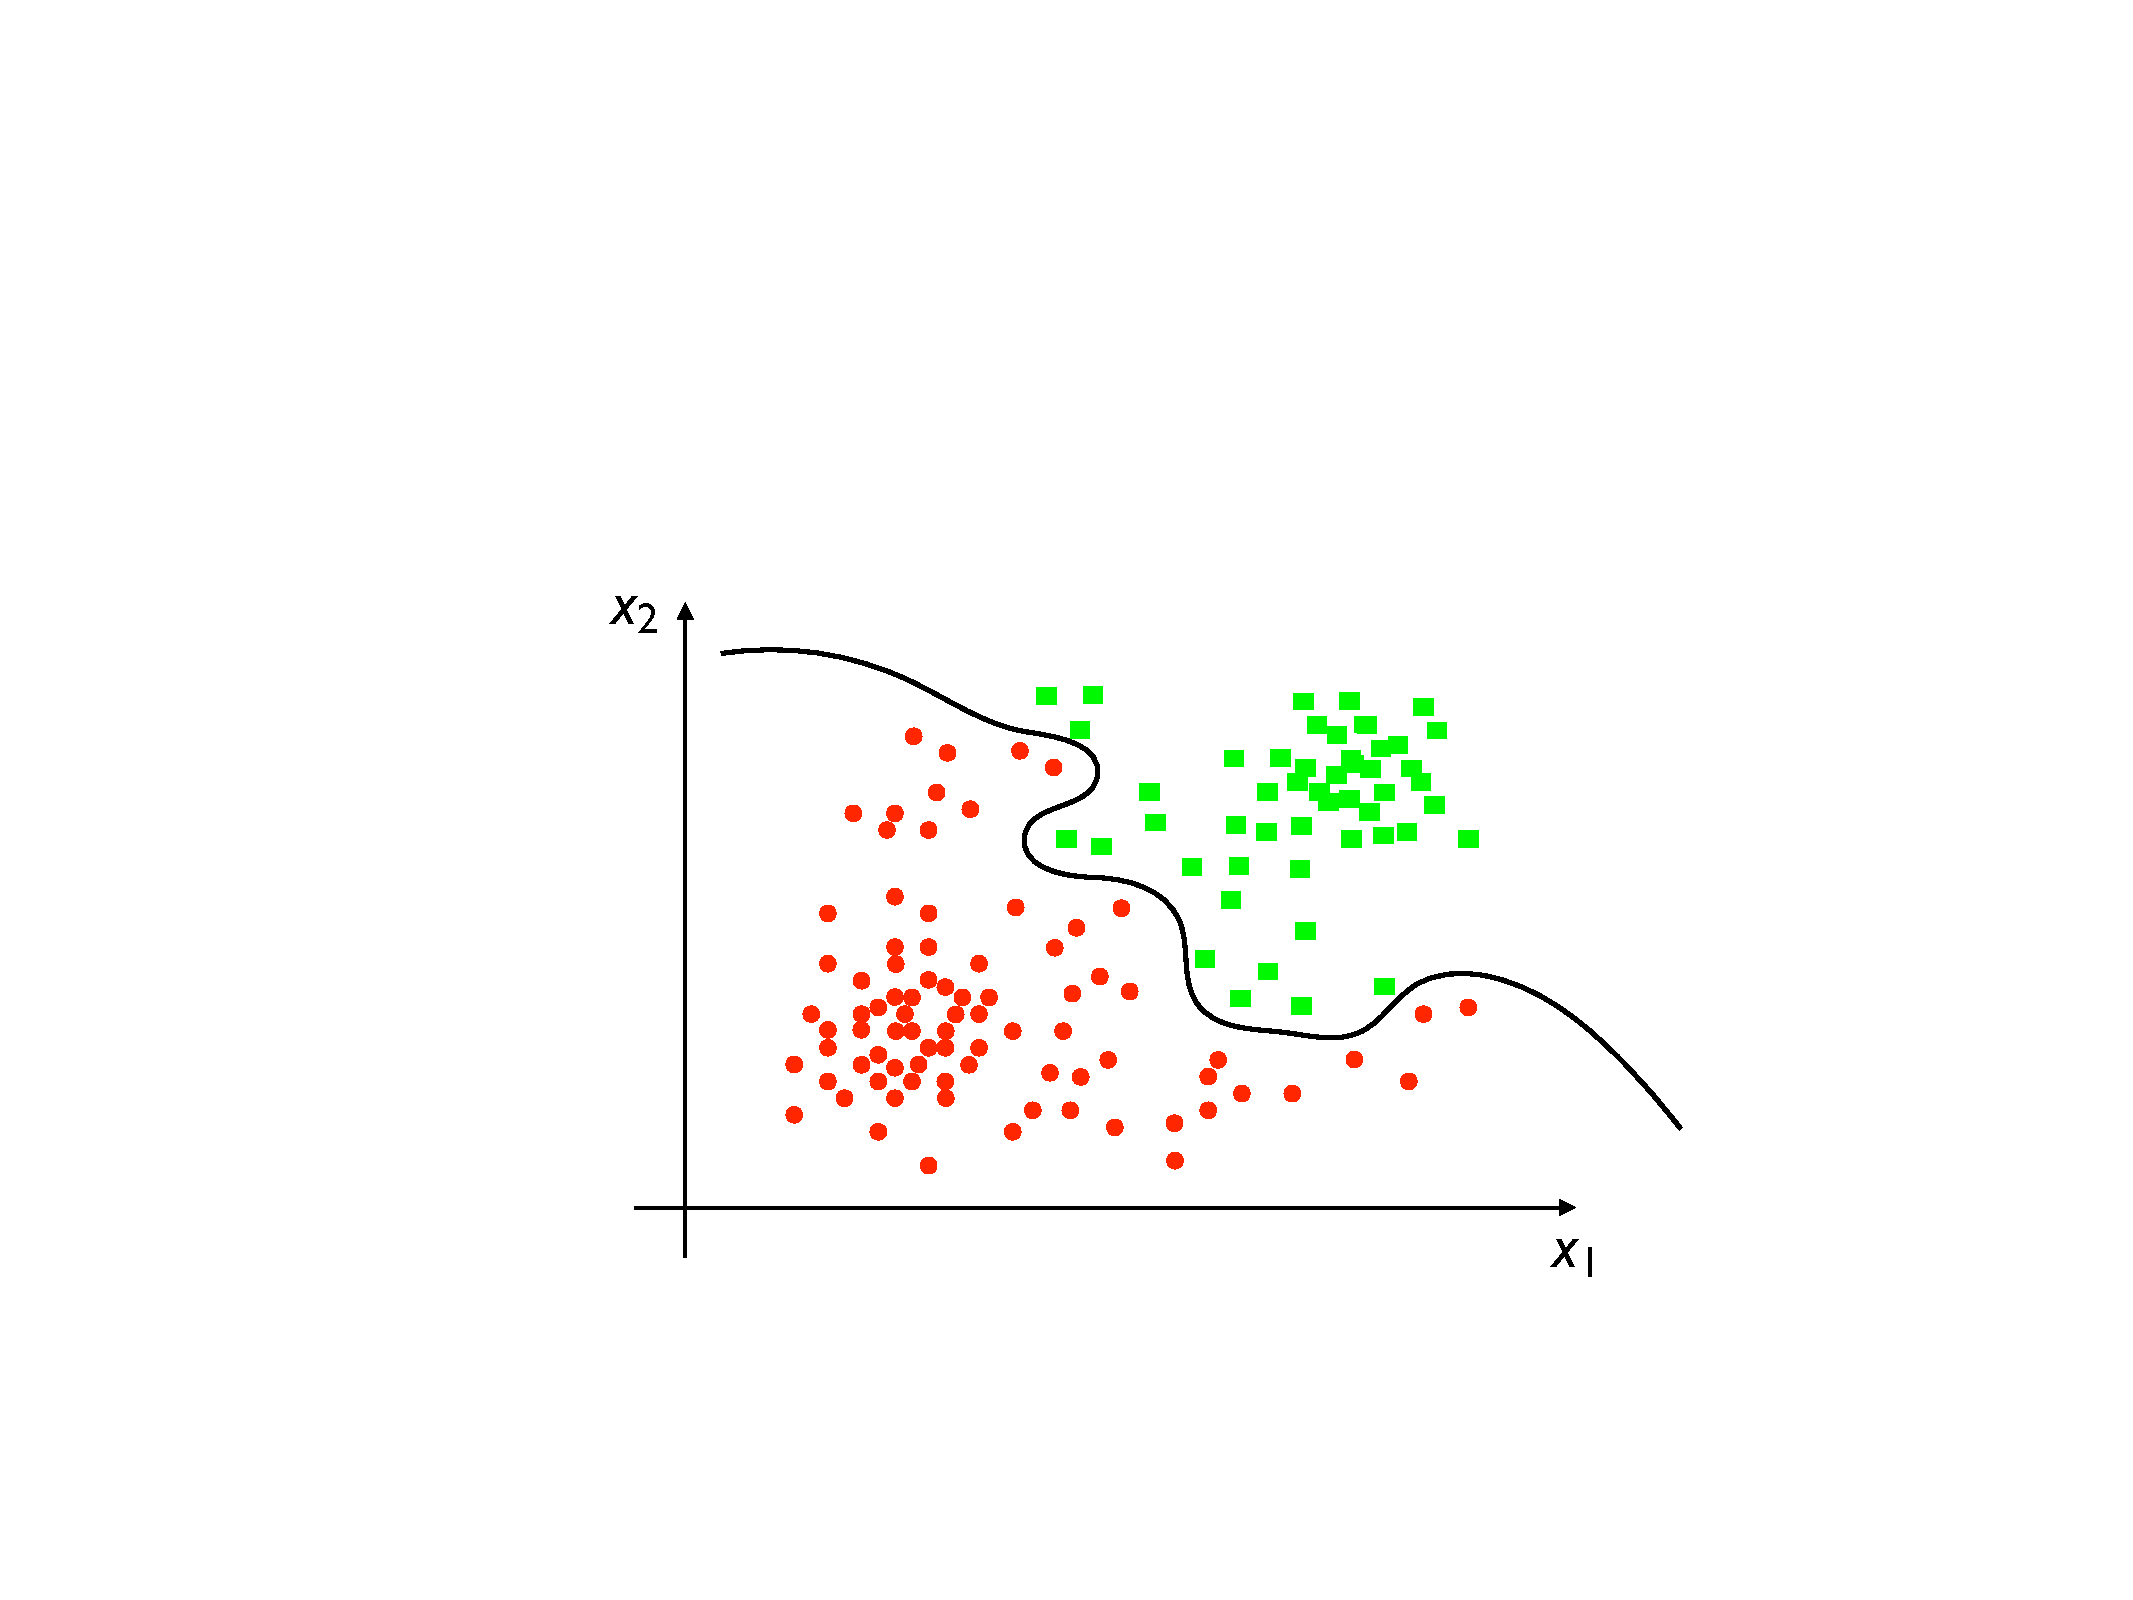
\includegraphics[height=0.3\textheight]{../graphics/Figure_supervised.pdf}} \hspace{1cm}
   		\subfloat{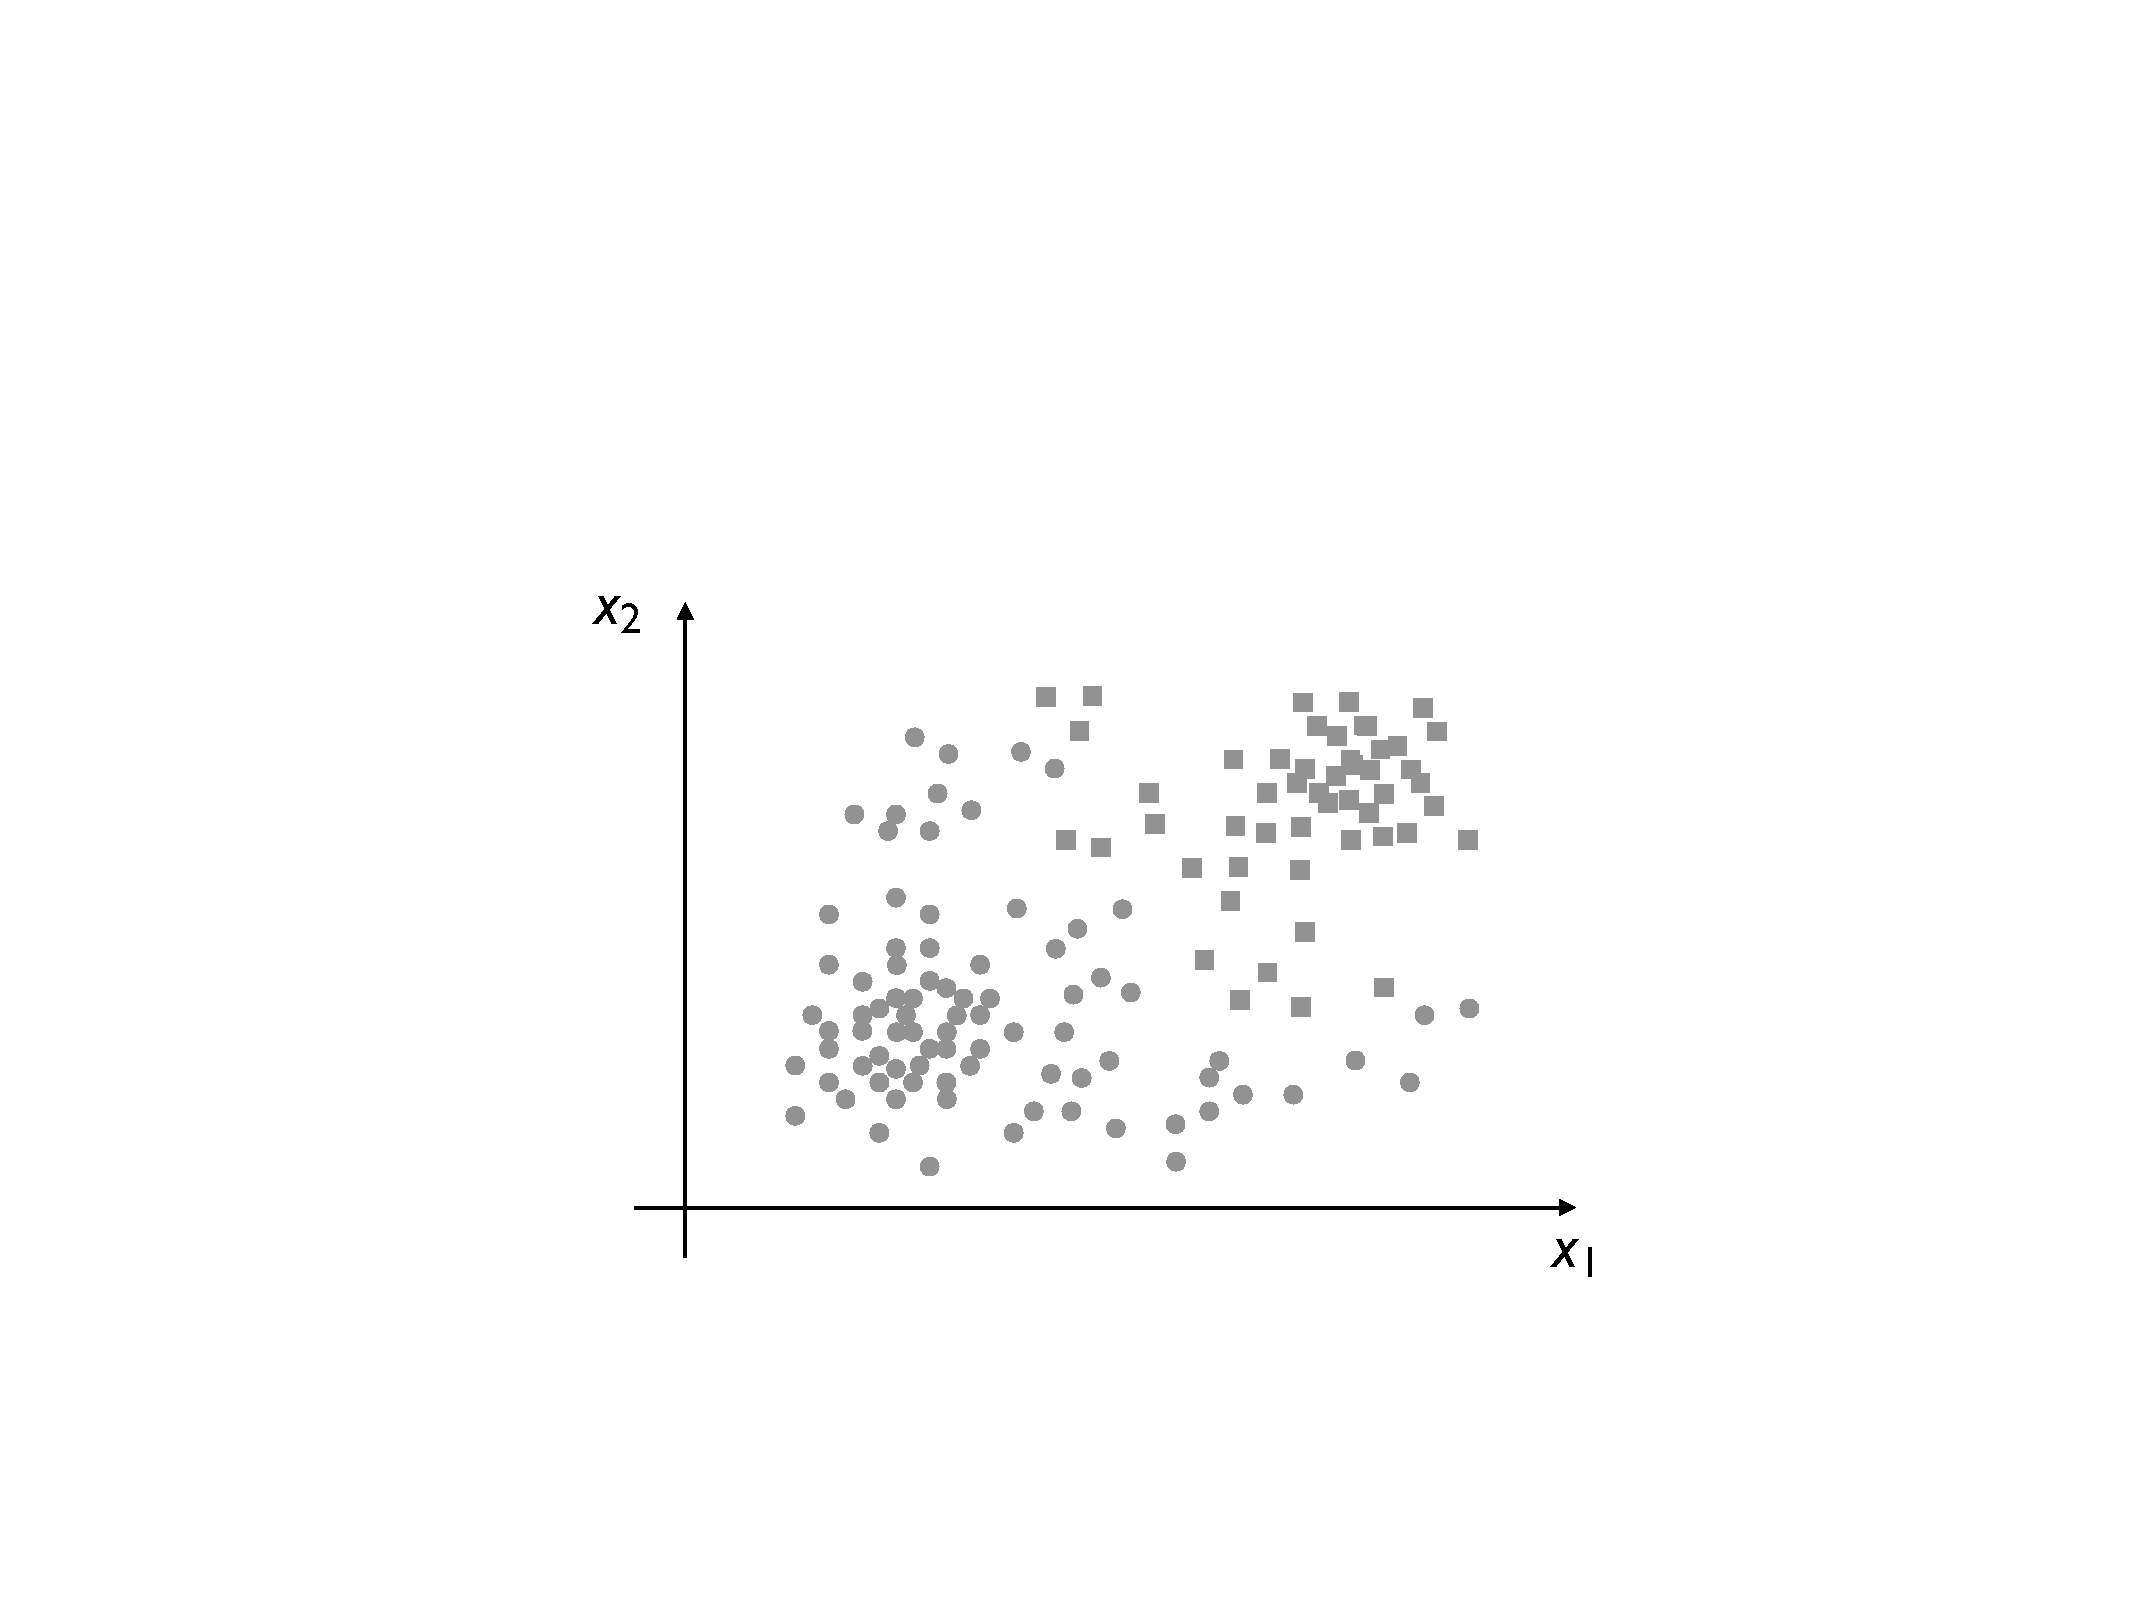
\includegraphics[height=0.3\textheight]{../graphics/Figure_unsupervised.pdf}}
   		\caption{Supervised and unsupervised learning}
	 \end{figure}
	Depending on the type of the output variable and on whether we are in a supervised or unsupervised setting, we have different names for machine learning problems:
	\begin{table}
	\begin{tabular}{|l || c | c | }
		\hline
 		& Supervised & Unsupervised \\
		\hline \hline
		$y$ labels & Classification & Clustering \\
		$y$ continuous & Regression & Dimensionality reduction\\
		\hline
	\end{tabular}
	\end{table}
\end{frame}

\begin{frame}{Objects and features}
\begin{itemize}
\item Machine learning typically deals with objects outside the mathematical world (emails, images, genomes, cars, $\ldots$).
\item The first step is therefore to find a suitable representation of the objects.
\begin{itemize}
\item \textbf{feature engineering}: finding descriptors according to existing domain knowledge
\item \textbf{representation learning}: learning the descriptors together with the classifier
\end{itemize}
\item In many cases the objects can be represented by a $\nfeatures$-dimensional vector of features (or descriptors): $\x \in \mathbb{R}^{\nfeatures}$.
\item It can be convenient to map a feature vector to a higher dimensional space:
\begin{eqnarray}
\featmap : \mathbb{R}^{\nfeatures} &\rightarrow & \mathbb{R}^Q \\
\x &\rightarrow &\featmap (\x)
\end{eqnarray}
\end{itemize}
\end{frame}

\begin{frame}{Example: classification of SPAM emails}
\begin{figure}[htb]
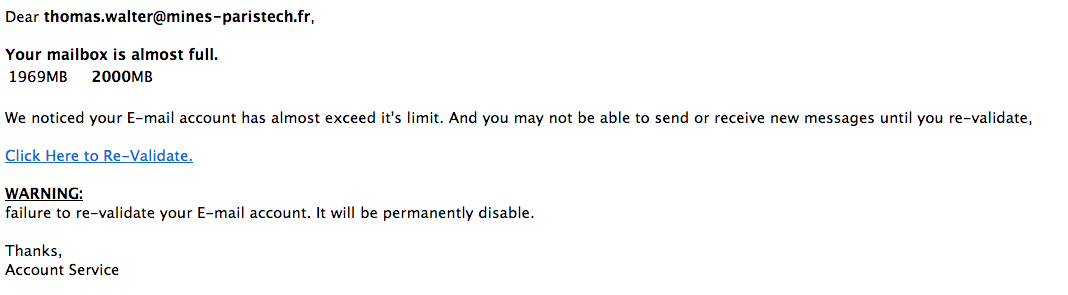
\includegraphics[width=0.9\textwidth]{../graphics/SPAM_mail.png}
\end{figure}
\begin{itemize}
	\item This is a binary classification problem: $y \in \{0,1\}$ (0: junk, 1: normal).
	\item The features can be constructed in the following way: for each email annotated by the user, the words are listed. An email is described as a vector of frequencies of these words.
	\item The system learns then a function that assigns to each vector of measured word frequencies the label $y$.
\end{itemize}
\end{frame}

\begin{frame}{Example: classification of drugs}
\begin{figure}[htb]
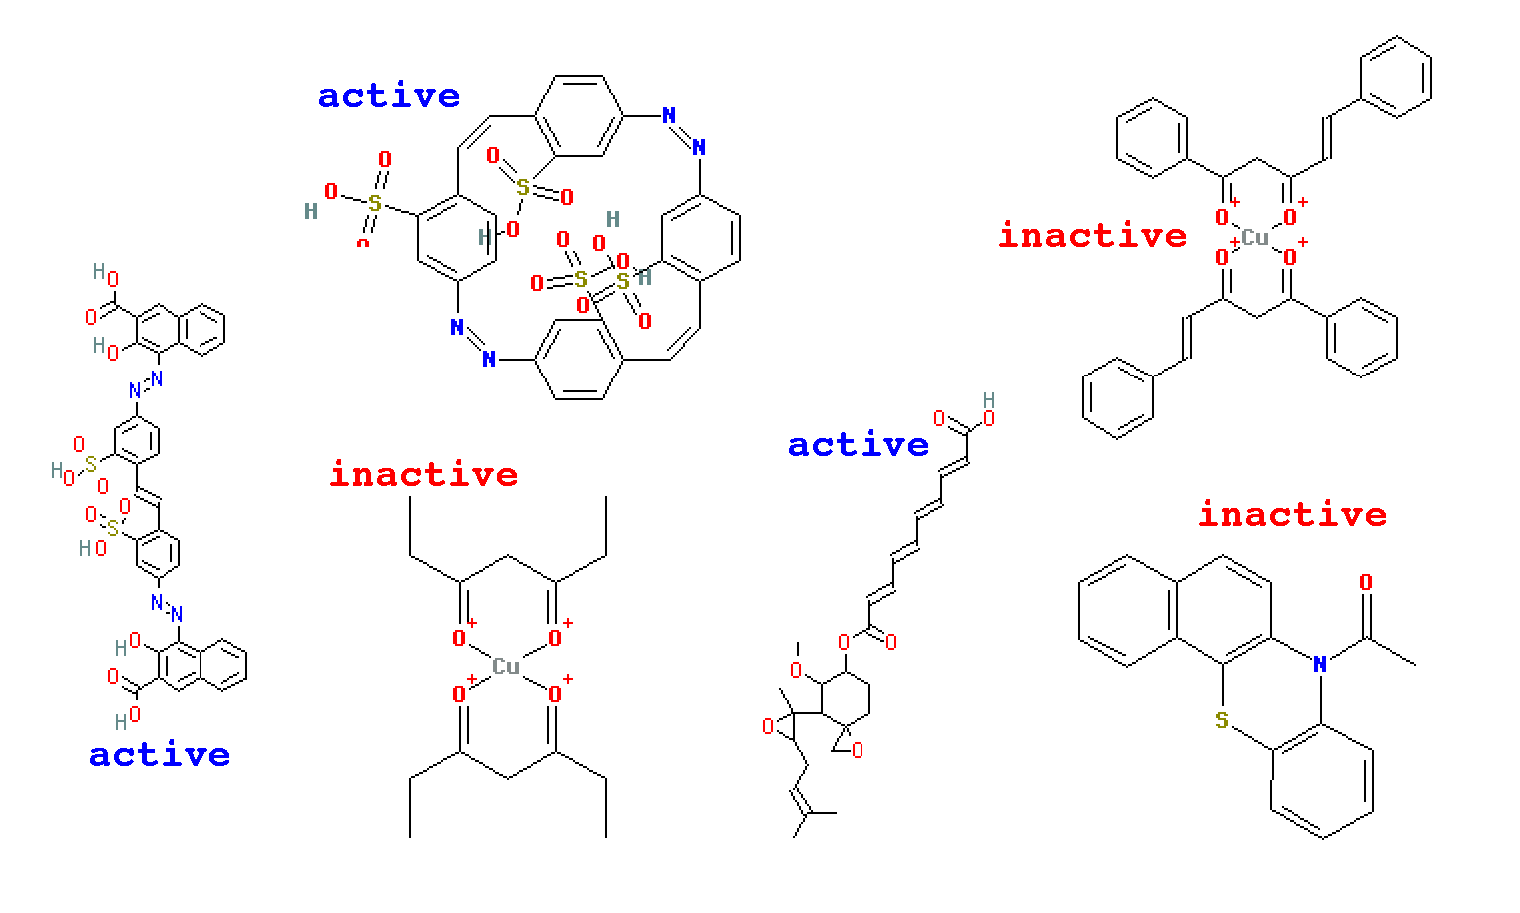
\includegraphics[width=0.7\textwidth]{../graphics/ml_example_drugs.pdf}
\end{figure}
\begin{itemize}
	\item Here, we want to classify molecules with respect to their efficiency against a disease (binary classification: a drug is efficient or not).
	\item An important question here is how to encode a molecule. One option is to define chemoinformatic features and obtain a vectorial representation of the molecule $\x \in \mathbb{R}^{\nfeatures}$.
\end{itemize}
\end{frame}


%%%%%%%%%%%%%%%%%%%%%%%%%%%%%%%%%%%%%%%%%%%%%%%%%%%%%%%%%%%%%%%%%%%%%%%%%
%%%%%%%%%%%%%%%%%%%%%%%%%%%%%%%%%%%%%%%%%%%%%%%%%%%%%%%%%%%%%%%%%%%%%%%%%
\section{Application examples from medical imaging}
\frame{\frametitle{Overview}\tableofcontents[currentsection]}
\begin{frame}{An example from  medical diagnostics: radiology}
\begin{figure}[htb]
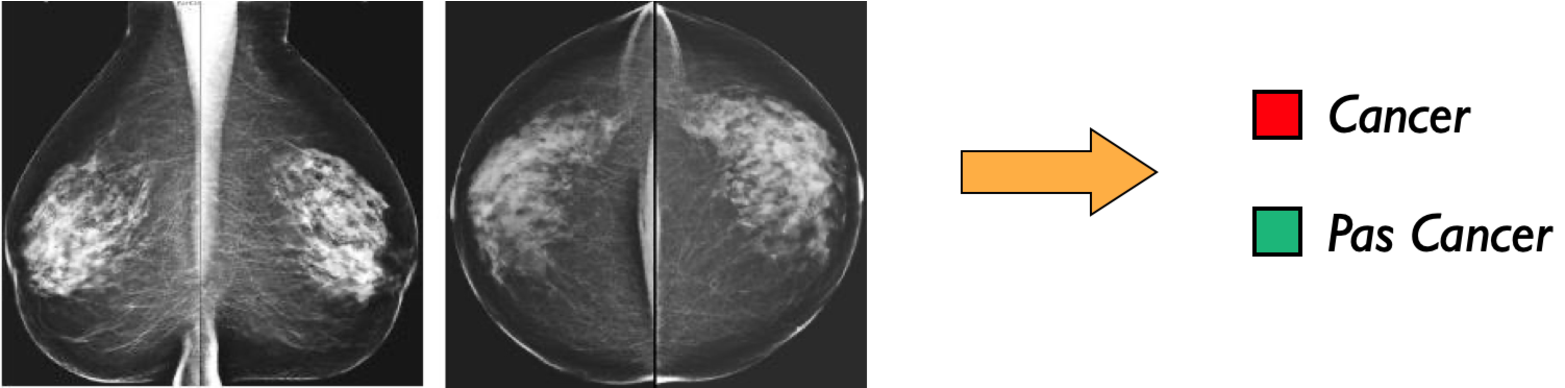
\includegraphics[width=0.8\textwidth]{../graphics/radiology.pdf}
\end{figure}

\begin{itemize}
\item<1-> Problem presented in an international challenge (won by Terapixel).
\item<2-> A Neural Networks trained on 640.000 images obtained an accuracy of 80\%. \
\item<3-> Problem ownership: who owns the trained network?
\item<4-> Problem responsibility: who is responsible in case of a wrong diagnosis?
\end{itemize}
\end{frame}

\begin{frame}{Skin cancer detection}
\begin{figure}[htb]
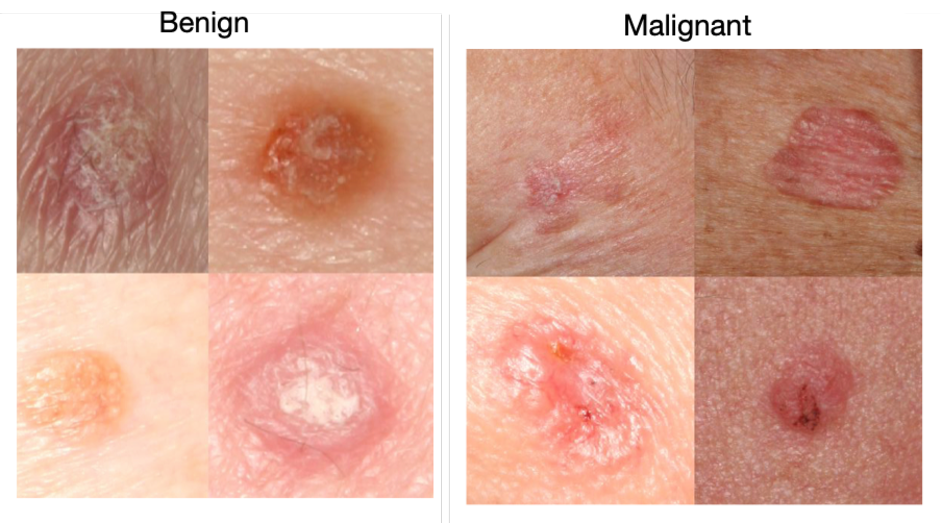
\includegraphics[width=0.6\textwidth]{../graphics/dermatology.pdf}
\end{figure}
\begin{itemize}
\item<1-> A Neural Network trained on 127 000 images was shown to outperform 21 dermatologists (72\% accuracy vs. 66\%) \cite{Esteva2017}
\item<2-> Improving healthcare or mass layoff of medical doctors?
\item<3-> Do the algorithms work equally well for different ethnic groups?
\end{itemize}
\end{frame}

\begin{frame}{What else can we predict?}
\begin{figure}[htb]
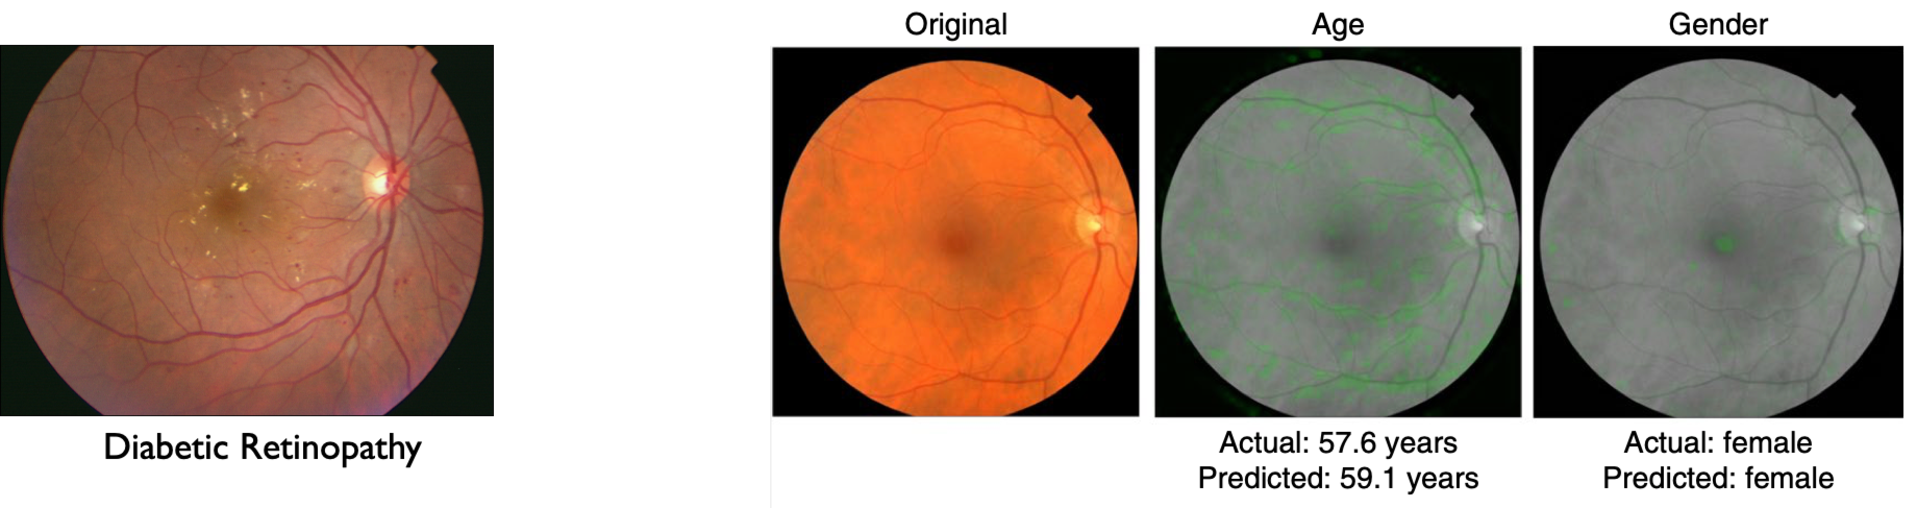
\includegraphics[width=0.9\textwidth]{../graphics/retinopathy.pdf}
\end{figure}
\begin{itemize}
\item<1-> A NN trained on 128.000 images reaches 87\% sensitivity and 91 \% specificity and became the first FDA approved autonomous IA medical device \cite{Abramoff2018}
\item<2-> From eye images, we can also predict age, BMI, cardiovascular risks and smoking habits \cite{Poplin2018}
\item<3-> What do we allow to predict? Who is using this information?
\end{itemize}
\end{frame}

\begin{frame}{Watson: should we stop thinking on our own?}
\begin{figure}[htb]
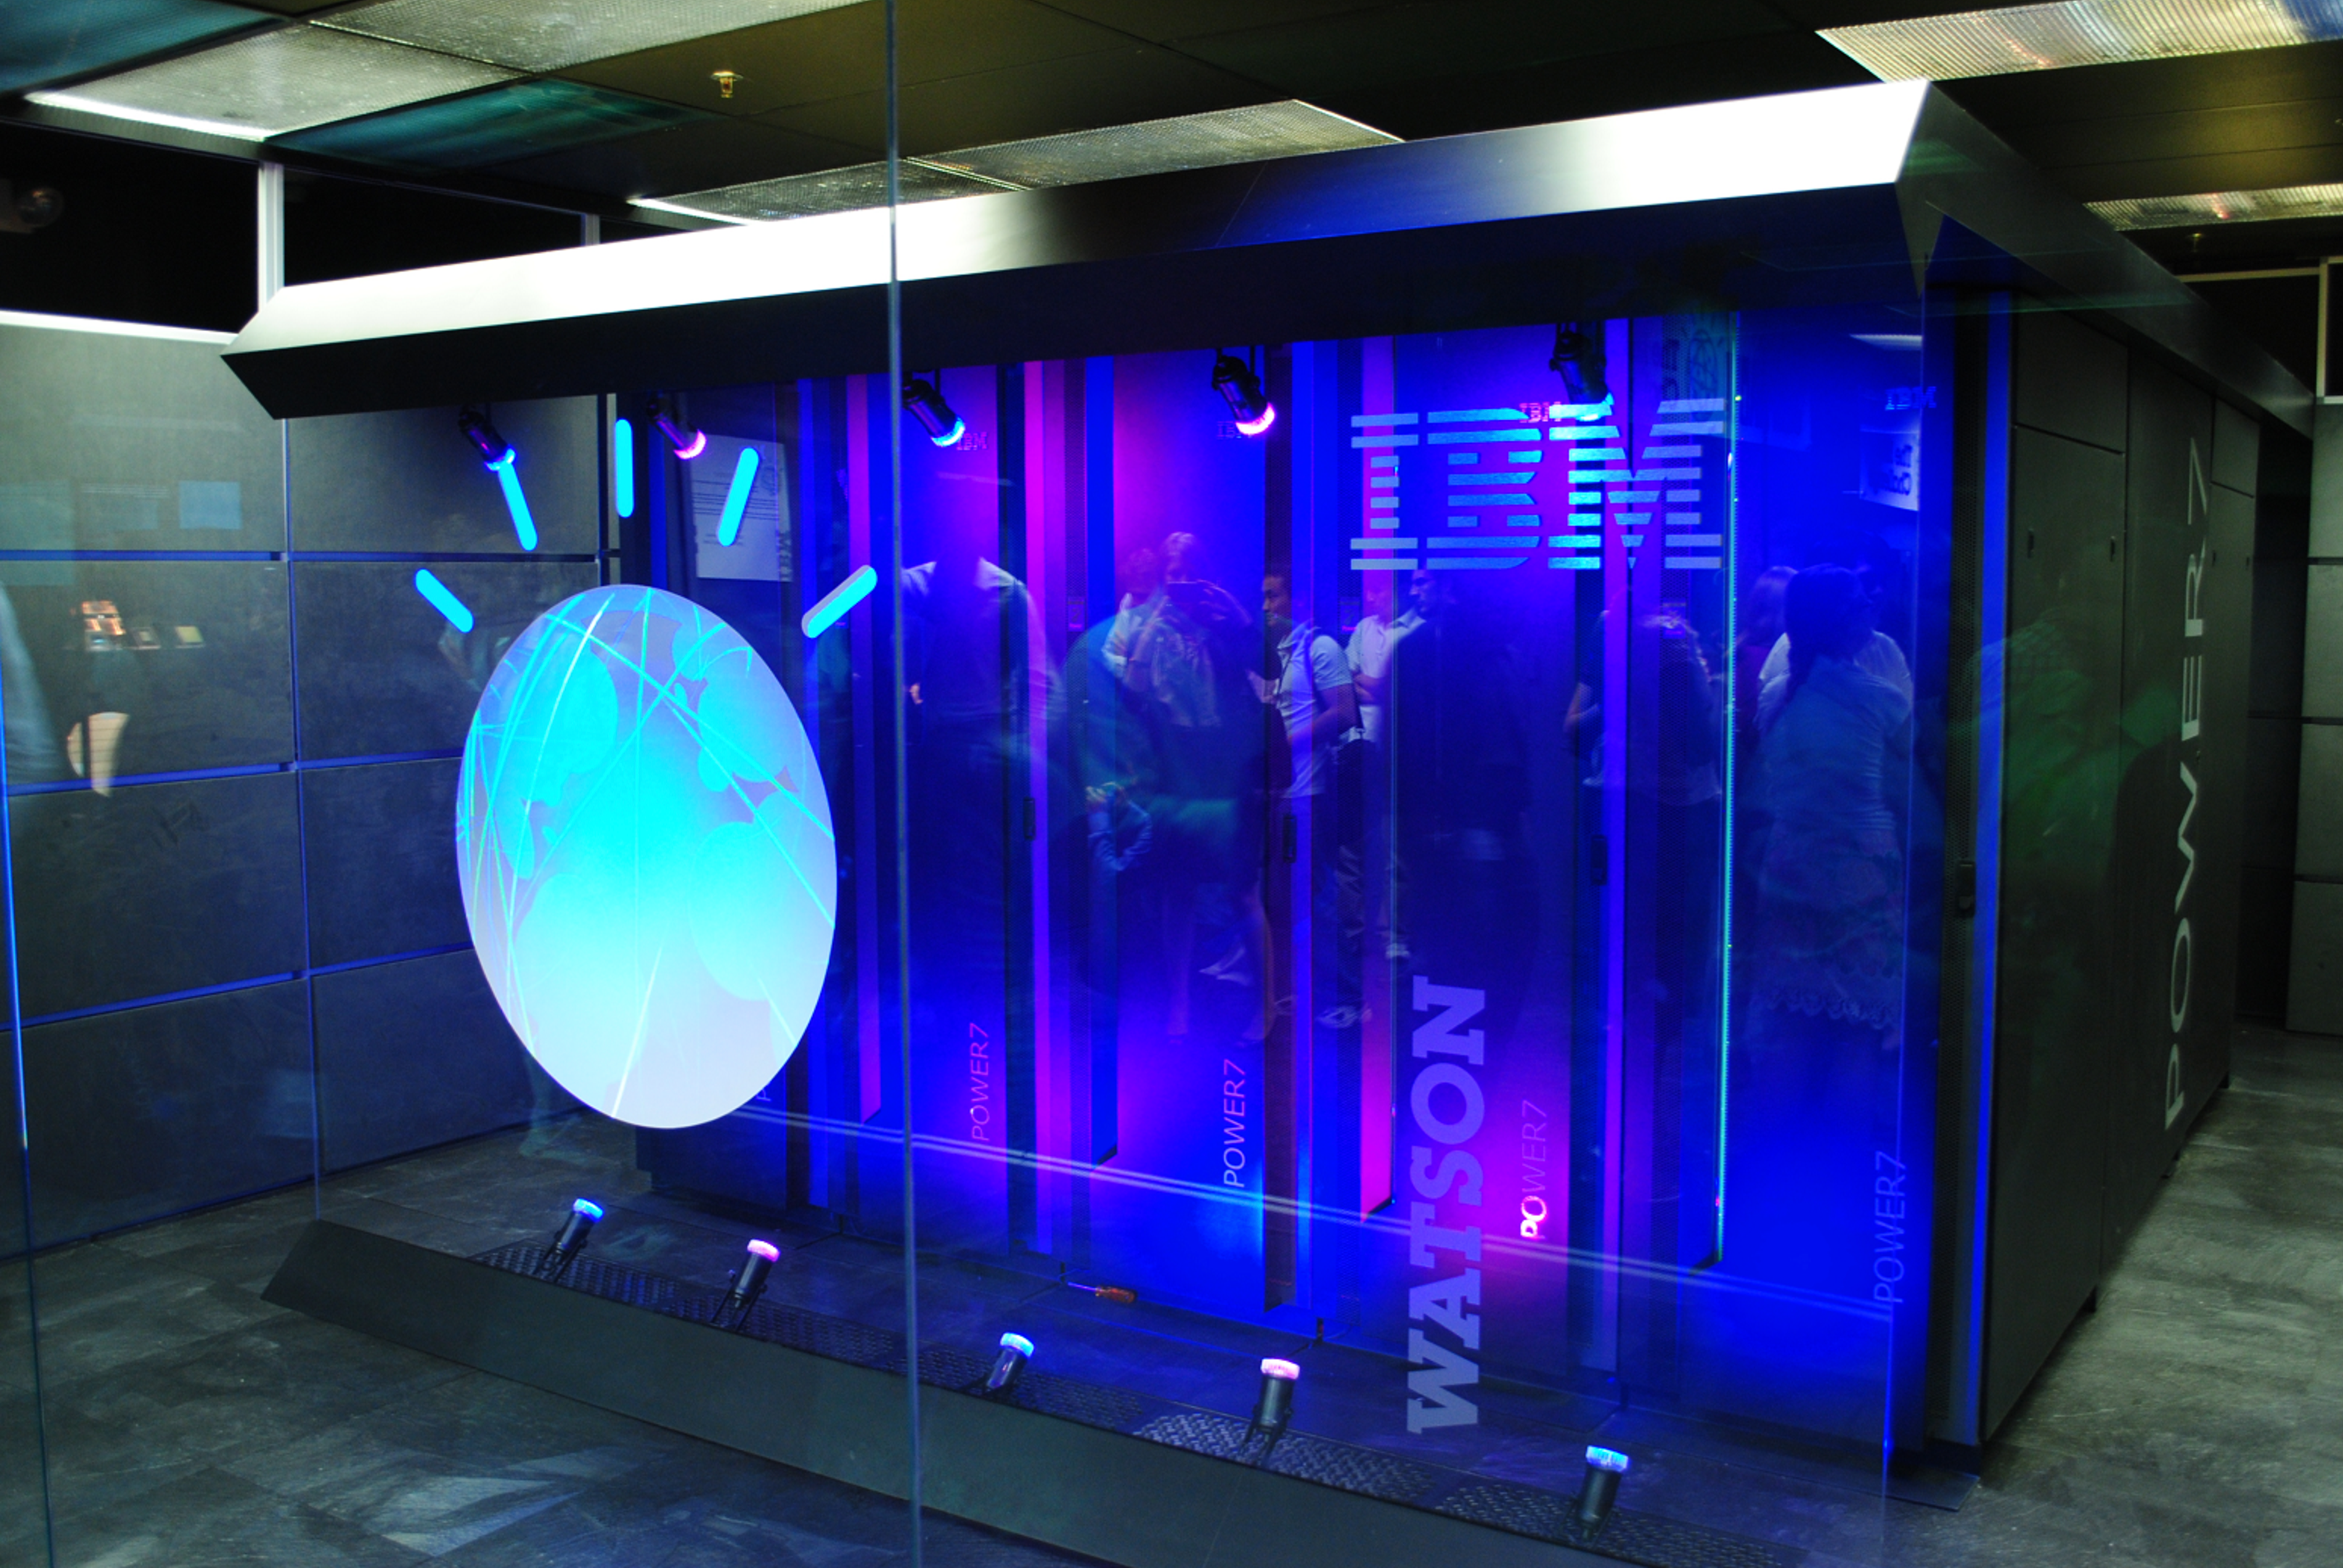
\includegraphics[width=0.5\textwidth]{../graphics/watson.pdf}
\end{figure}
\begin{itemize}
\item<1-> Watson (developed by IBM) outperformed humans in the game Jeopardy.
\item<2-> The system is used for clinical decision support (with usually good results).
\item<3-> Medical personnel usually follow the advice.
\end{itemize}
\end{frame}

\begin{frame}{Beyond the medical domain ... }
\begin{itemize}
\item AI for criminal risk assessment: predicting the likelihood  from the prisoners profiles. Problem: learning racist associations.
\item AI in autonomous driving:
\begin{itemize}
	\item Individual cases versus overall performance
	\item Responsibility in case of an accident
	\item Moral hard-coding
\end{itemize}
\item Generative Models for images: new tools for manipulations, mobbing, etc.
\item AI replacing humans: mass layouts?
\item $\ldots$
\end{itemize}

\end{frame}

% \begin{frame}{AI for criminal risk assessment}
% \begin{figure}[htb]
% 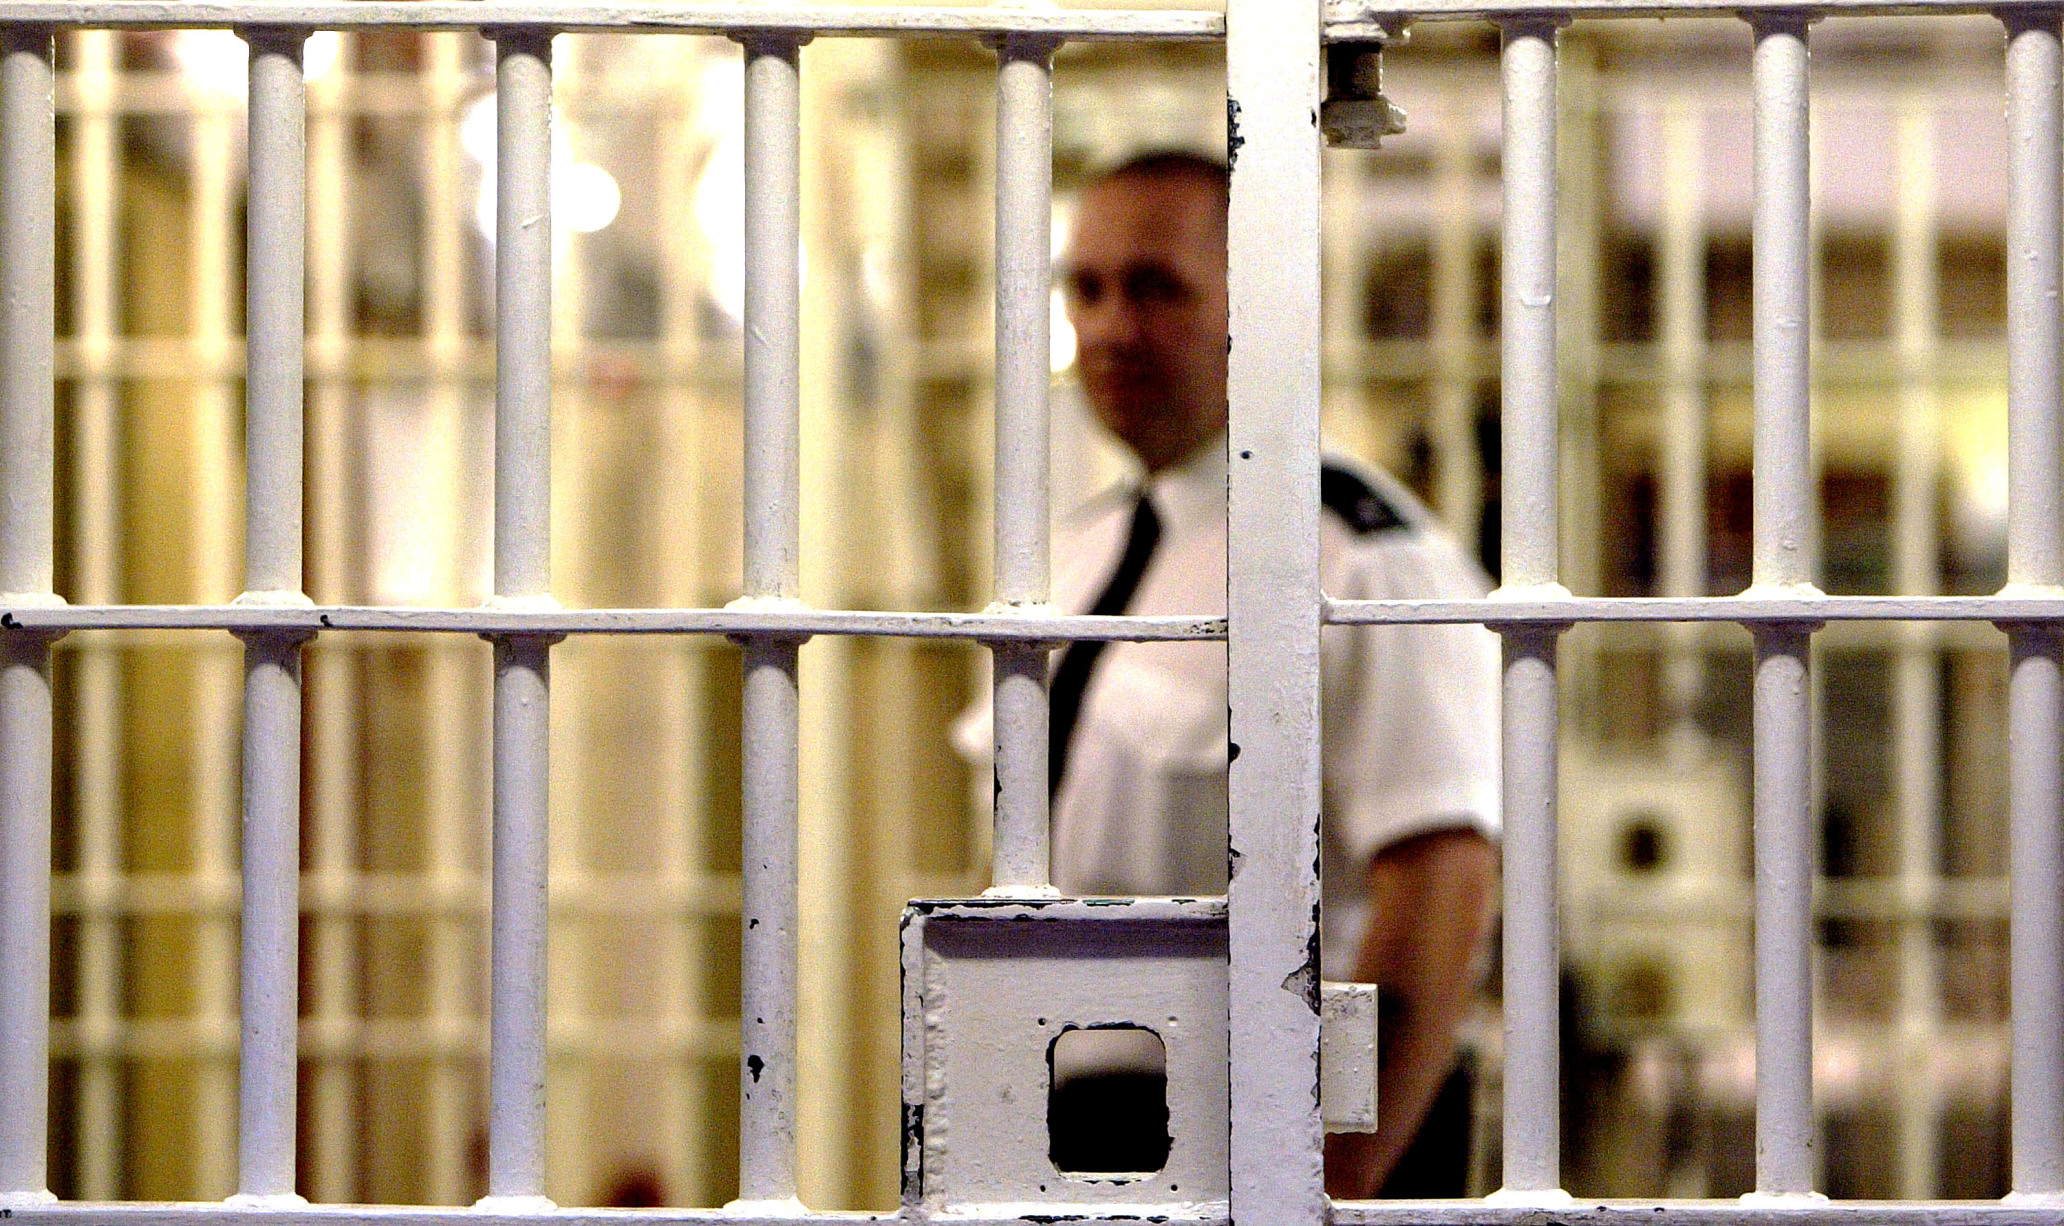
\includegraphics[width=0.5\textwidth]{../graphics/jail.jpg}
% \end{figure}
% \begin{itemize}
% \item<1-> Predict the likelihood of recidivism from the prisoners profile.
% \item<2-> Overall, the algorithms tend to outperform humans \cite{Lin2020}.
% \item<3-> However, they might learn "racist" associations due to the statistical composition of the training set.
% \end{itemize}
% \end{frame}



%%%%%%%%%%%%%%%%%%%%%%%%%%%%%%%%%%%%%%%%%%%%%%%%%%%%%%%%%%%%%%%%%%%%%%%%%
%%%%%%%%%%%%%%%%%%%%%%%%%%%%%%%%%%%%%%%%%%%%%%%%%%%%%%%%%%%%%%%%%%%%%%%%%
\section{Design Principles of Machine Learning algorithms}
\frame{\frametitle{Overview}\tableofcontents[currentsection]}

\begin{frame}{A simple example: polynomial curve fitting\footnote{Example adapted from \cite{Bishop2006}}}
\begin{figure}[htb]
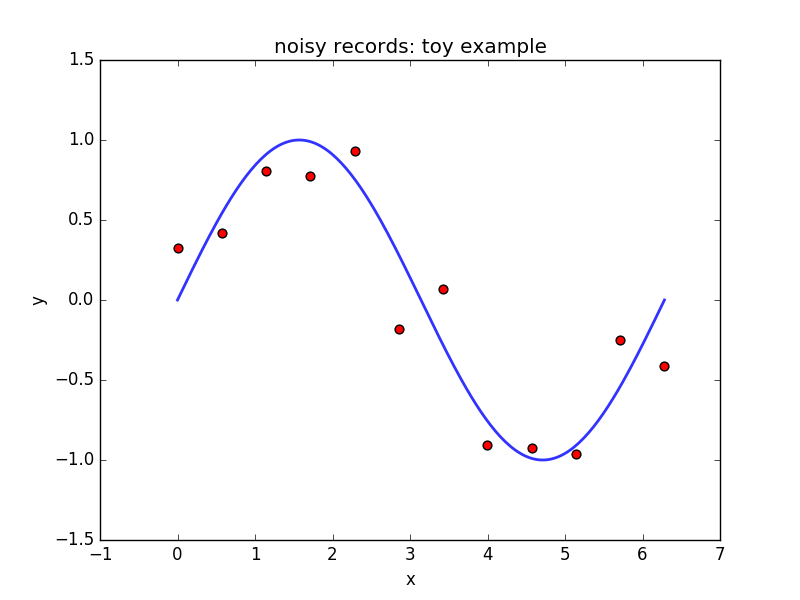
\includegraphics[width=0.6\textwidth]{../graphics/sample_from_sin.png}
\end{figure}
\begin{itemize}
	\item From a set of measured points $(x_i, y_i)$ (red), we would like to build a model to predict the value $y$ for any given $x$.
	%% \item The true function is $g(x)=\sin (x)$ (displayed in blue).
	%% \item The measurements $y_i$ are noisy outputs of that function, i.e.
	%% \begin{equation}
	%% y_i = \sin (x_i) + \epsilon \; , \;\;\; \;\;\; \epsilon \sim \mathcal{N}(0,0.2)
	%% \end{equation}
\end{itemize}
\end{frame}

\begin{frame}{A simple example: polynomial curve fitting}
\begin{itemize}
	\item<1-> We use the following polynomial model:
	\begin{eqnarray}
	f(x) &=& a_0 + a_1 x + a_2 x^2 + \ldots + a_m x^m \nonumber \\
	&=& \param^T \featmap (x)
	\end{eqnarray}
	\item<2-> Parameter vector: $\param = (a_0, a_1, \ldots, a_m)^T$
	\item<3-> Here, the initial measurement $x$ is a scalar. In our model, we map $x$ to a higher dimensional space:
	\begin{eqnarray}
		\featmap : \mathbb{R}^{\nfeatures} &\rightarrow & \mathbb{R}^Q \nonumber \\
		x &\rightarrow & \featmap (x) = (1, x, x^2, \ldots, x^m)^T
	\end{eqnarray}
	\item<4-> The model is linear in the parameters $\theta$ and linear in $\featmap$, but for $m>1$, the model is not linear in $x$.
\end{itemize}
\end{frame}

\begin{frame}{A simple example: polynomial curve fitting}
\begin{itemize}
	\item<1-> One classical approach is to minimize the least squared error between measured and predicted values:
	\begin{eqnarray}
		\min_{\param} \loss(\param) &=& \min_{\param} \sum_{i=1}^N (y_i - f(x_i))^2 \nonumber \\
		&=& \min_{\param} \sum_{i=1}^N (y_i - \param^T \featmap (x_i))^2
	\end{eqnarray}
	\item<2-> This can be achieved by setting the gradient with respect to $\param$ to zero:
	\begin{equation}
		\nabla_{\param} \loss = (\frac{\partial \loss}{\partial a_0}, \frac{\partial \loss}{\partial a_1}, \ldots, \frac{\partial \loss}{\partial a_m} )^T = 0
	\end{equation}
	\item<3-> Unlike for most optimization problems in this course, this leads to an analytical solution for $\param$. This is known as \textbf{linear regression}. For more details, we refer to \cite{Hastie2009}.
\end{itemize}
\end{frame}

\begin{frame}{Overfitting and underfitting}
\begin{columns}
\begin{column}{.8\textwidth}
\begin{figure}[htb]
	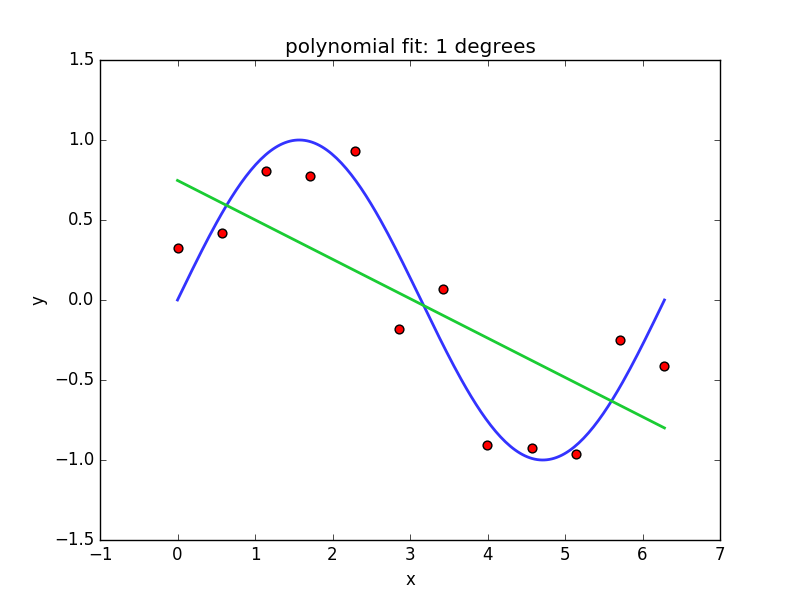
\includegraphics[width=0.75\textwidth]{../graphics/polyfit_degree_1.png}
\end{figure}
\end{column}
\begin{column}{.2\textwidth}
$\| \param \|^2 = 0.67$
\end{column}
\end{columns}
For $m=1$ the solution is not capable of modeling the measured data points; we get a poor approximation of the original function. The family of functions we have used was not complex enough to model the true data distribution. We also speak of \textbf{underfitting}.
%\begin{textblock}{0}(.9\textwidth,\paperheight)
%  Test
% \end{textblock}
\end{frame}

\begin{frame}{Overfitting and underfitting}
\begin{columns}
\begin{column}{.8\textwidth}
\begin{figure}[htb]
	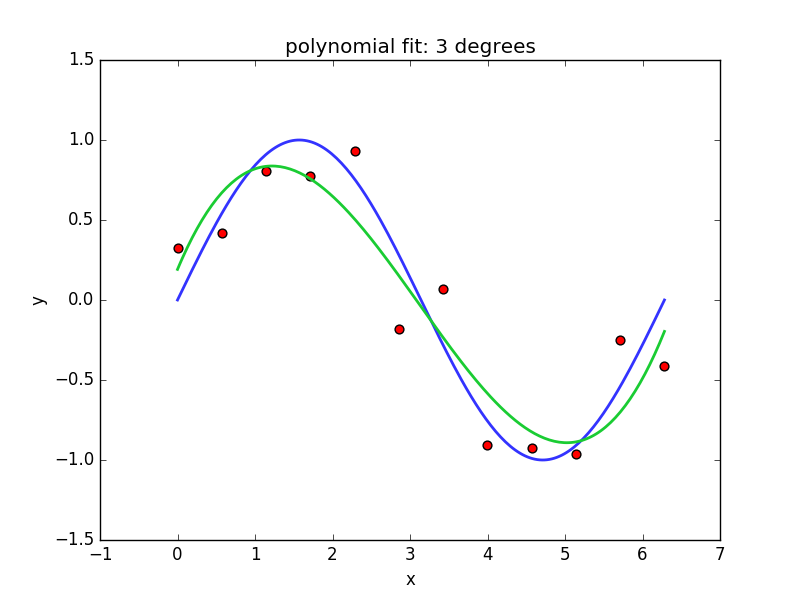
\includegraphics[width=0.75\textwidth]{../graphics/polyfit_degree_3.png}
\end{figure}
\end{column}
\begin{column}{.2\textwidth}
$\| \param \|^2 = 1.72$
\end{column}
\end{columns}
For $m=3$, we obtain a solution that seems to be quite right: it is sufficiently complex to model the true data distribution, but not too complex to model the small variations which are due to noise.
\end{frame}

\begin{frame}{Overfitting and underfitting}
\begin{columns}
\begin{column}{.8\textwidth}
\begin{figure}[htb]
	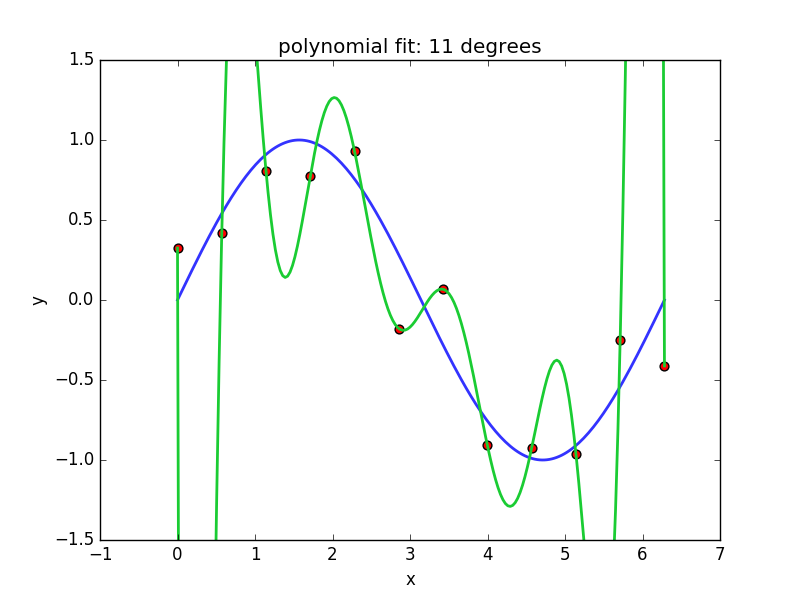
\includegraphics[width=0.75\textwidth]{../graphics/polyfit_degree_11.png}
\end{figure}
\end{column}
\begin{column}{.2\textwidth}
$\| \param \|^2 \approx 10^7$
\end{column}
\end{columns}
For $m=11$, we obtain a solution that has zero error (the function passes through every point of the training set). But the coefficients with large absolute values that cancel each other precisely on the training points lead to a highly unstable function. We speak of \textbf{overfitting} and \textbf{poor generalization}.
\end{frame}

\begin{frame}{Overfitting and underfitting}
\begin{columns}
\begin{column}{.8\textwidth}
\begin{figure}[htb]
	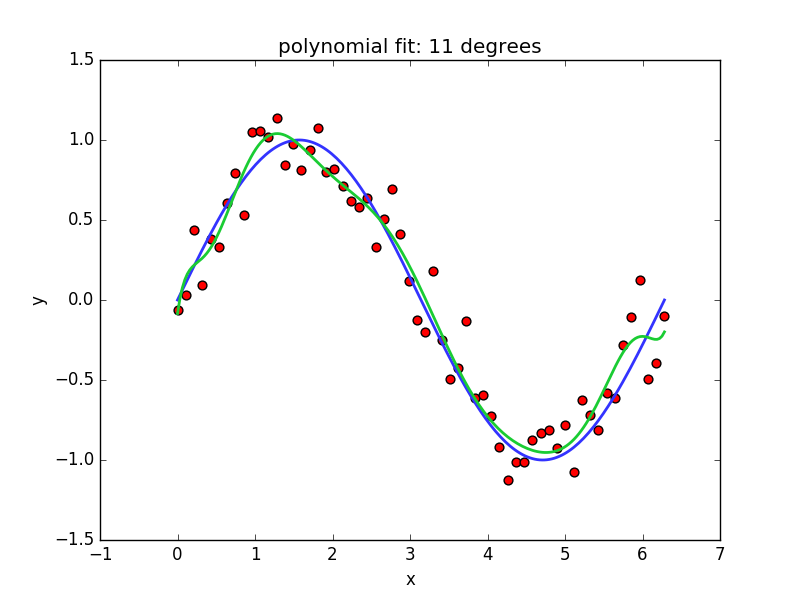
\includegraphics[width=0.75\textwidth]{../graphics/polyfit_degree_11_N60.png}
\end{figure}
\end{column}
\begin{column}{.2\textwidth}
$\| \param \|^2 = 5647$
\end{column}
\end{columns}
One way of reducing overfitting is to increase the number of samples. Even if the function is complex, it cannot be “too wild”, as it has to find a compromise between many training samples. This however implies the annotation (or measurement) of more samples.
\end{frame}

\begin{frame}{Overfitting and underfitting}
\begin{columns}
\begin{column}{.8\textwidth}
\begin{figure}[htb]
	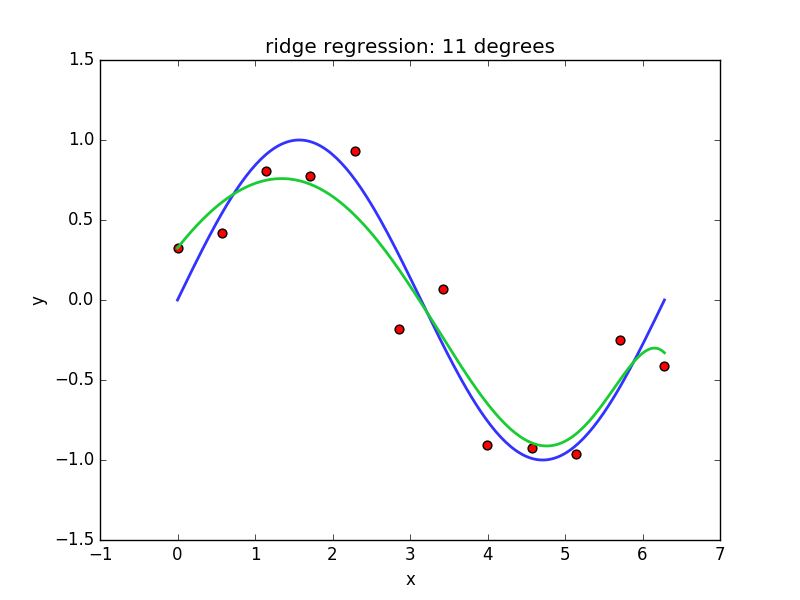
\includegraphics[width=0.75\textwidth]{../graphics/ridge_regression_11_10.png}
\end{figure}
\end{column}
\begin{column}{.2\textwidth}
$\| \param \|^2 = 0.41$
\end{column}
\end{columns}
Another way of preventing overfitting without increasing the number of samples, is to add a penalization term in the optimization procedure. This is also known as \textbf{regularization}:
\begin{equation}
	\loss = \sum_{i=1}^N (y_i - \param^T \featmap (x_i))^2 + \lambda \| \param \|^2
\end{equation}
\end{frame}

\begin{frame}{Generalization: training and test error}
\begin{figure}[htb]
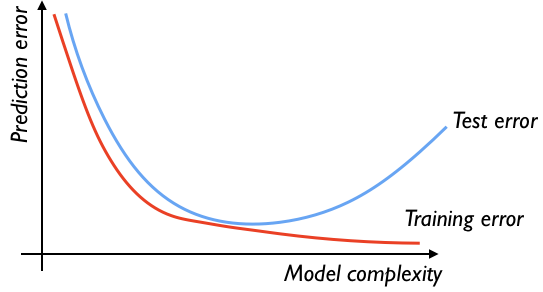
\includegraphics[width=0.6\textwidth]{../graphics/Training_and_test_error.png}
\end{figure}
\begin{itemize}
\item Supervised Learning aims at finding a function $f$ that predicts an output value $y$ from a measurement $x$ for unseen data, i.e. for data that has not been used to find $f$.
\item Machine Learning is much concerned with avoiding $f$ to \textbf{memorize} the training set, i.e. to perform well on a training set but poorly a test set.
\item An important paradigm is that we must never evaluate the performance of our machine learning method on the data that has been used to train it.
\end{itemize}
\end{frame}

\begin{frame}{Generalization: strategies}
\begin{itemize}
\item Many ML algorithms can be written as an optimization problem:
\begin{equation*}
\param ^{\ast} = \argmin_{\param} \loss (\param) + \lambda \mathcal{R}(\param)
\end{equation*}
Minimizing the loss $\loss (\param)$ aims at finding the rule to reproduce the annotations in the training set, minimizing the regularization term $\mathcal{R}(\param)$ aims at avoiding the model to adapt too much to the training data, leading to simpler models. We have seen the $L_2$ norm, but there are many other options for $\mathcal{R}$.
\item Other regularization strategies include:
\begin{itemize}
\item Model averaging (ensemble methods)
\item Artificial or actual increase of training data
\end{itemize}
\end{itemize}
\end{frame}

\section{Model evaluation and hyperparameters}
\frame{\frametitle{Overview}\tableofcontents[currentsection]}


% \begin{frame}{Model evaluation}
% 	\begin{figure}[htb]
% 		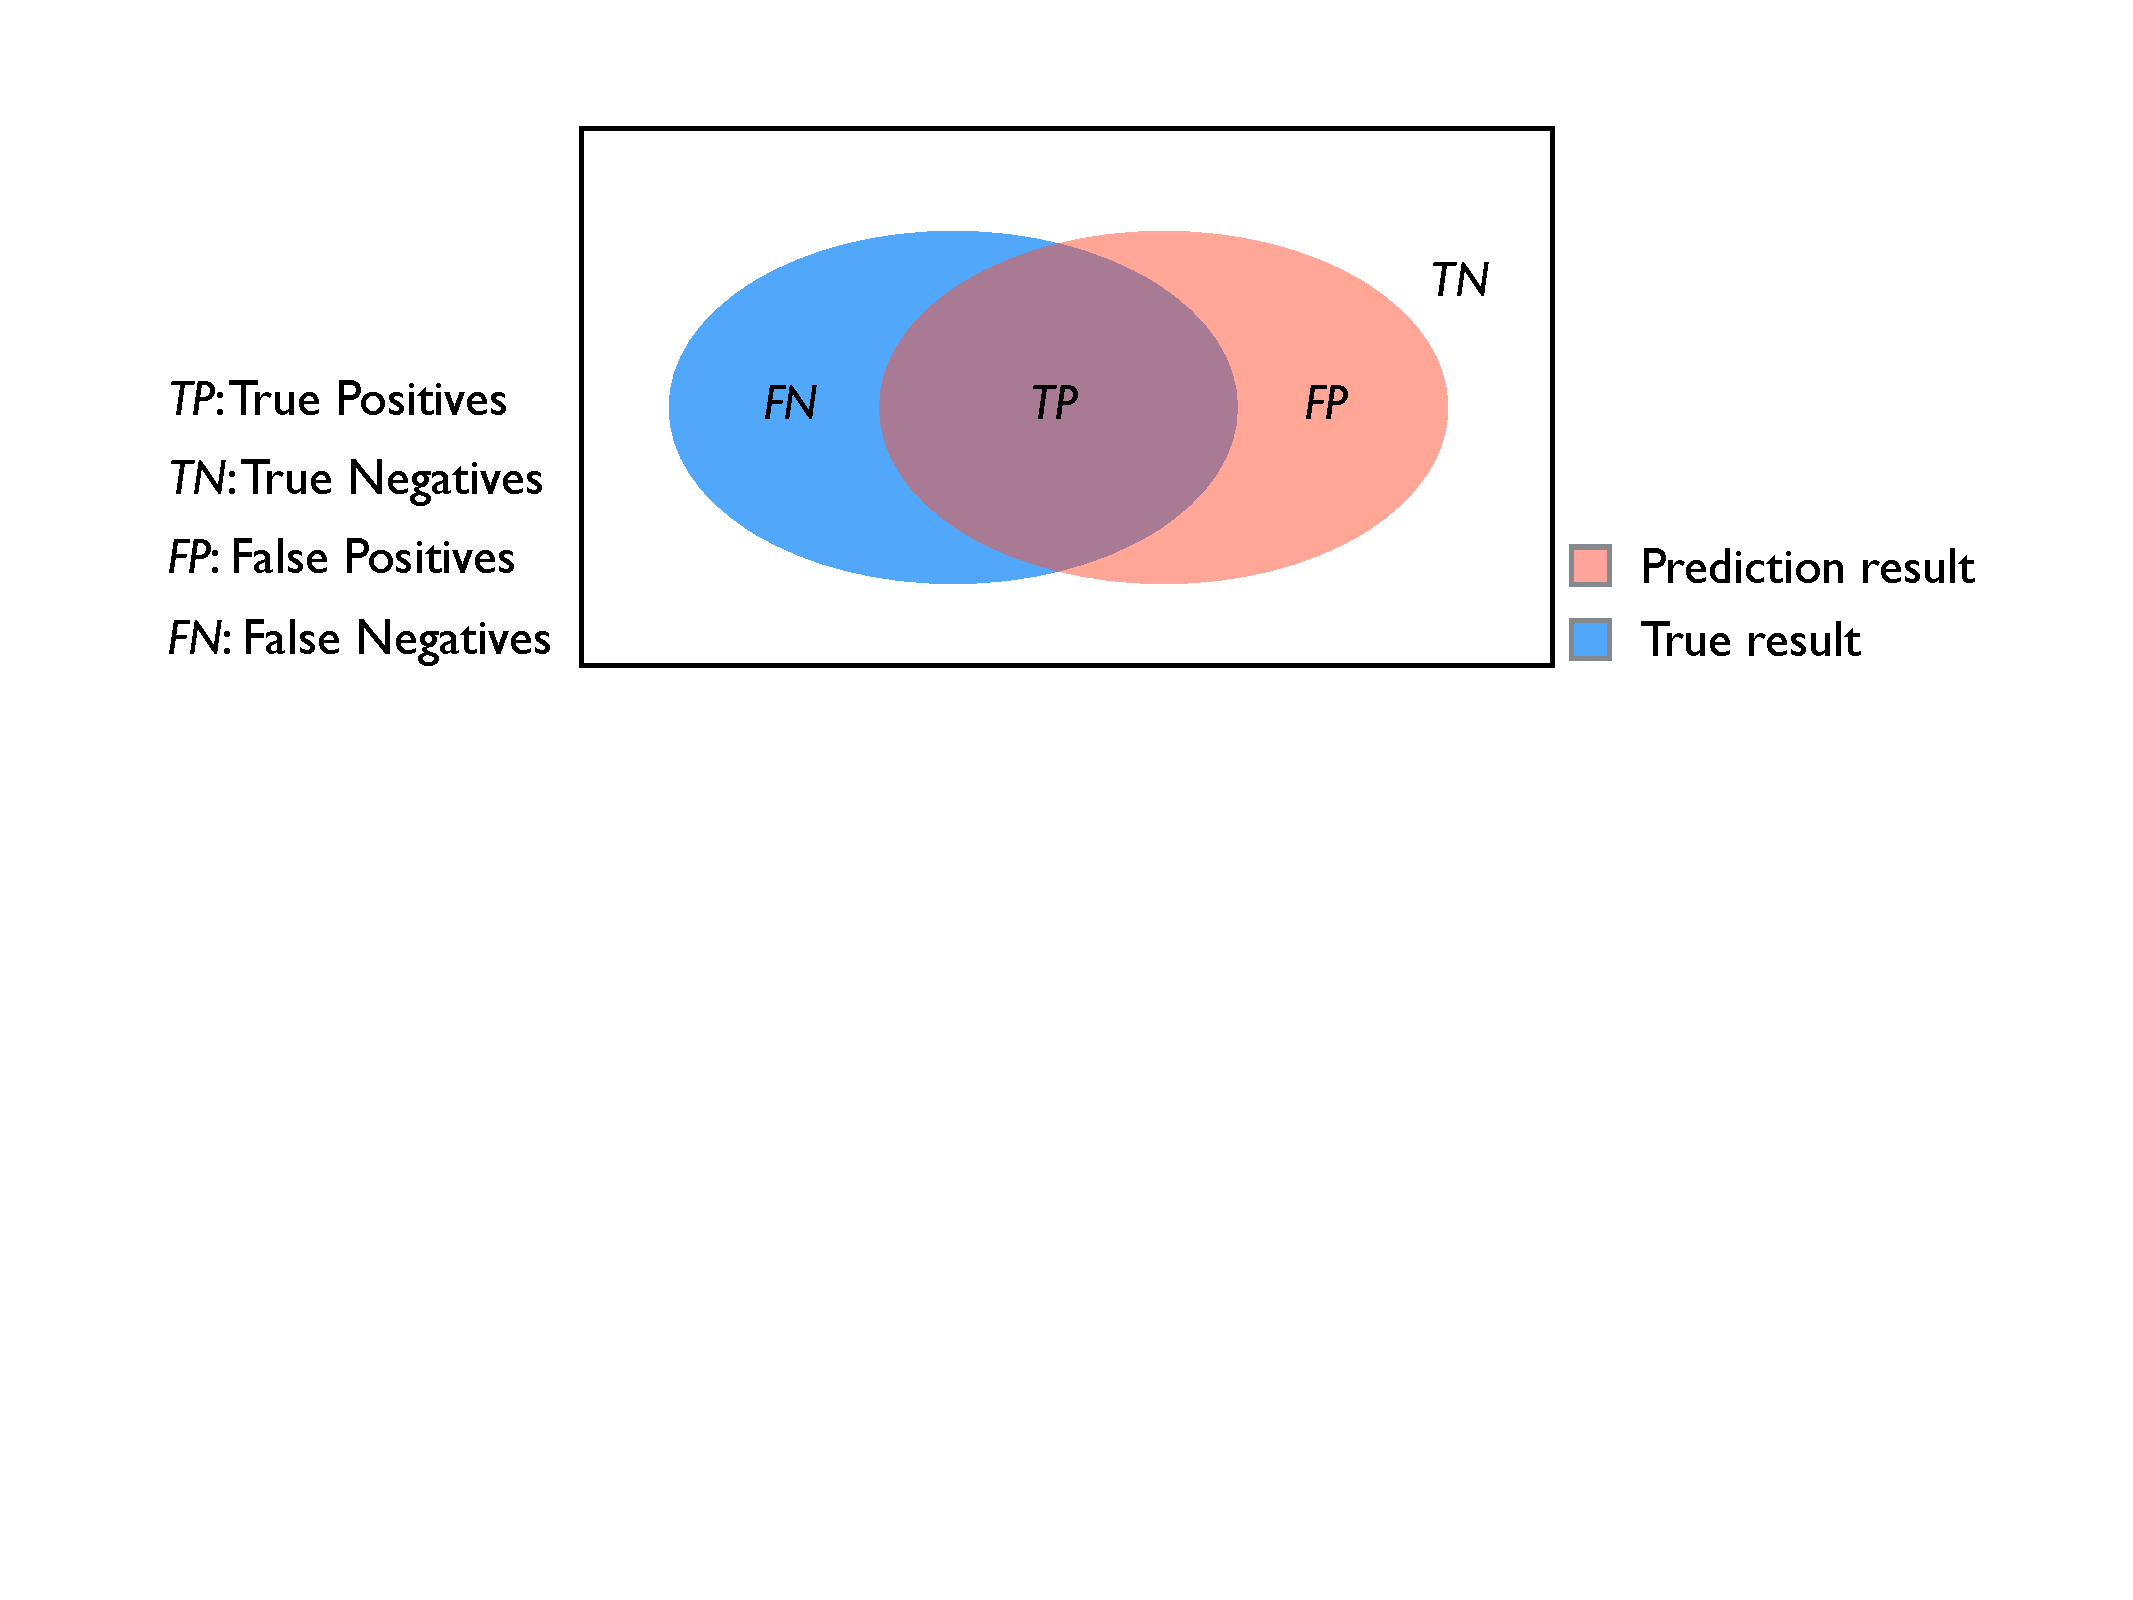
\includegraphics[width=0.9\textwidth]{../graphics/ModelEvaluation.pdf}
% 	\end{figure}
% 	\begin{itemize}
% 		\item First, we need suitable metrics to evaluate a model's performance.
% 		\item The following metrics are used often:
% 		\begin{eqnarray*}
% 		\text{recall} &=& \frac{TP}{TP + FN} \\
% 		\text{precision} &=& \frac{TP}{TP + FP} \\
% 		\text{accuracy} &=& \frac{TP + TN}{TP + TN + FP + FN} \\
% 		%F1 = &=& 2 \cdot \frac{\text{recall}\cdot\text{precision}}{\text{recall} + \text{precision}}
% 		\end{eqnarray*}
% 	\end{itemize}
% \end{frame}

\begin{frame}{Model evaluation - Accuracy}
	\begin{figure}[htb]
		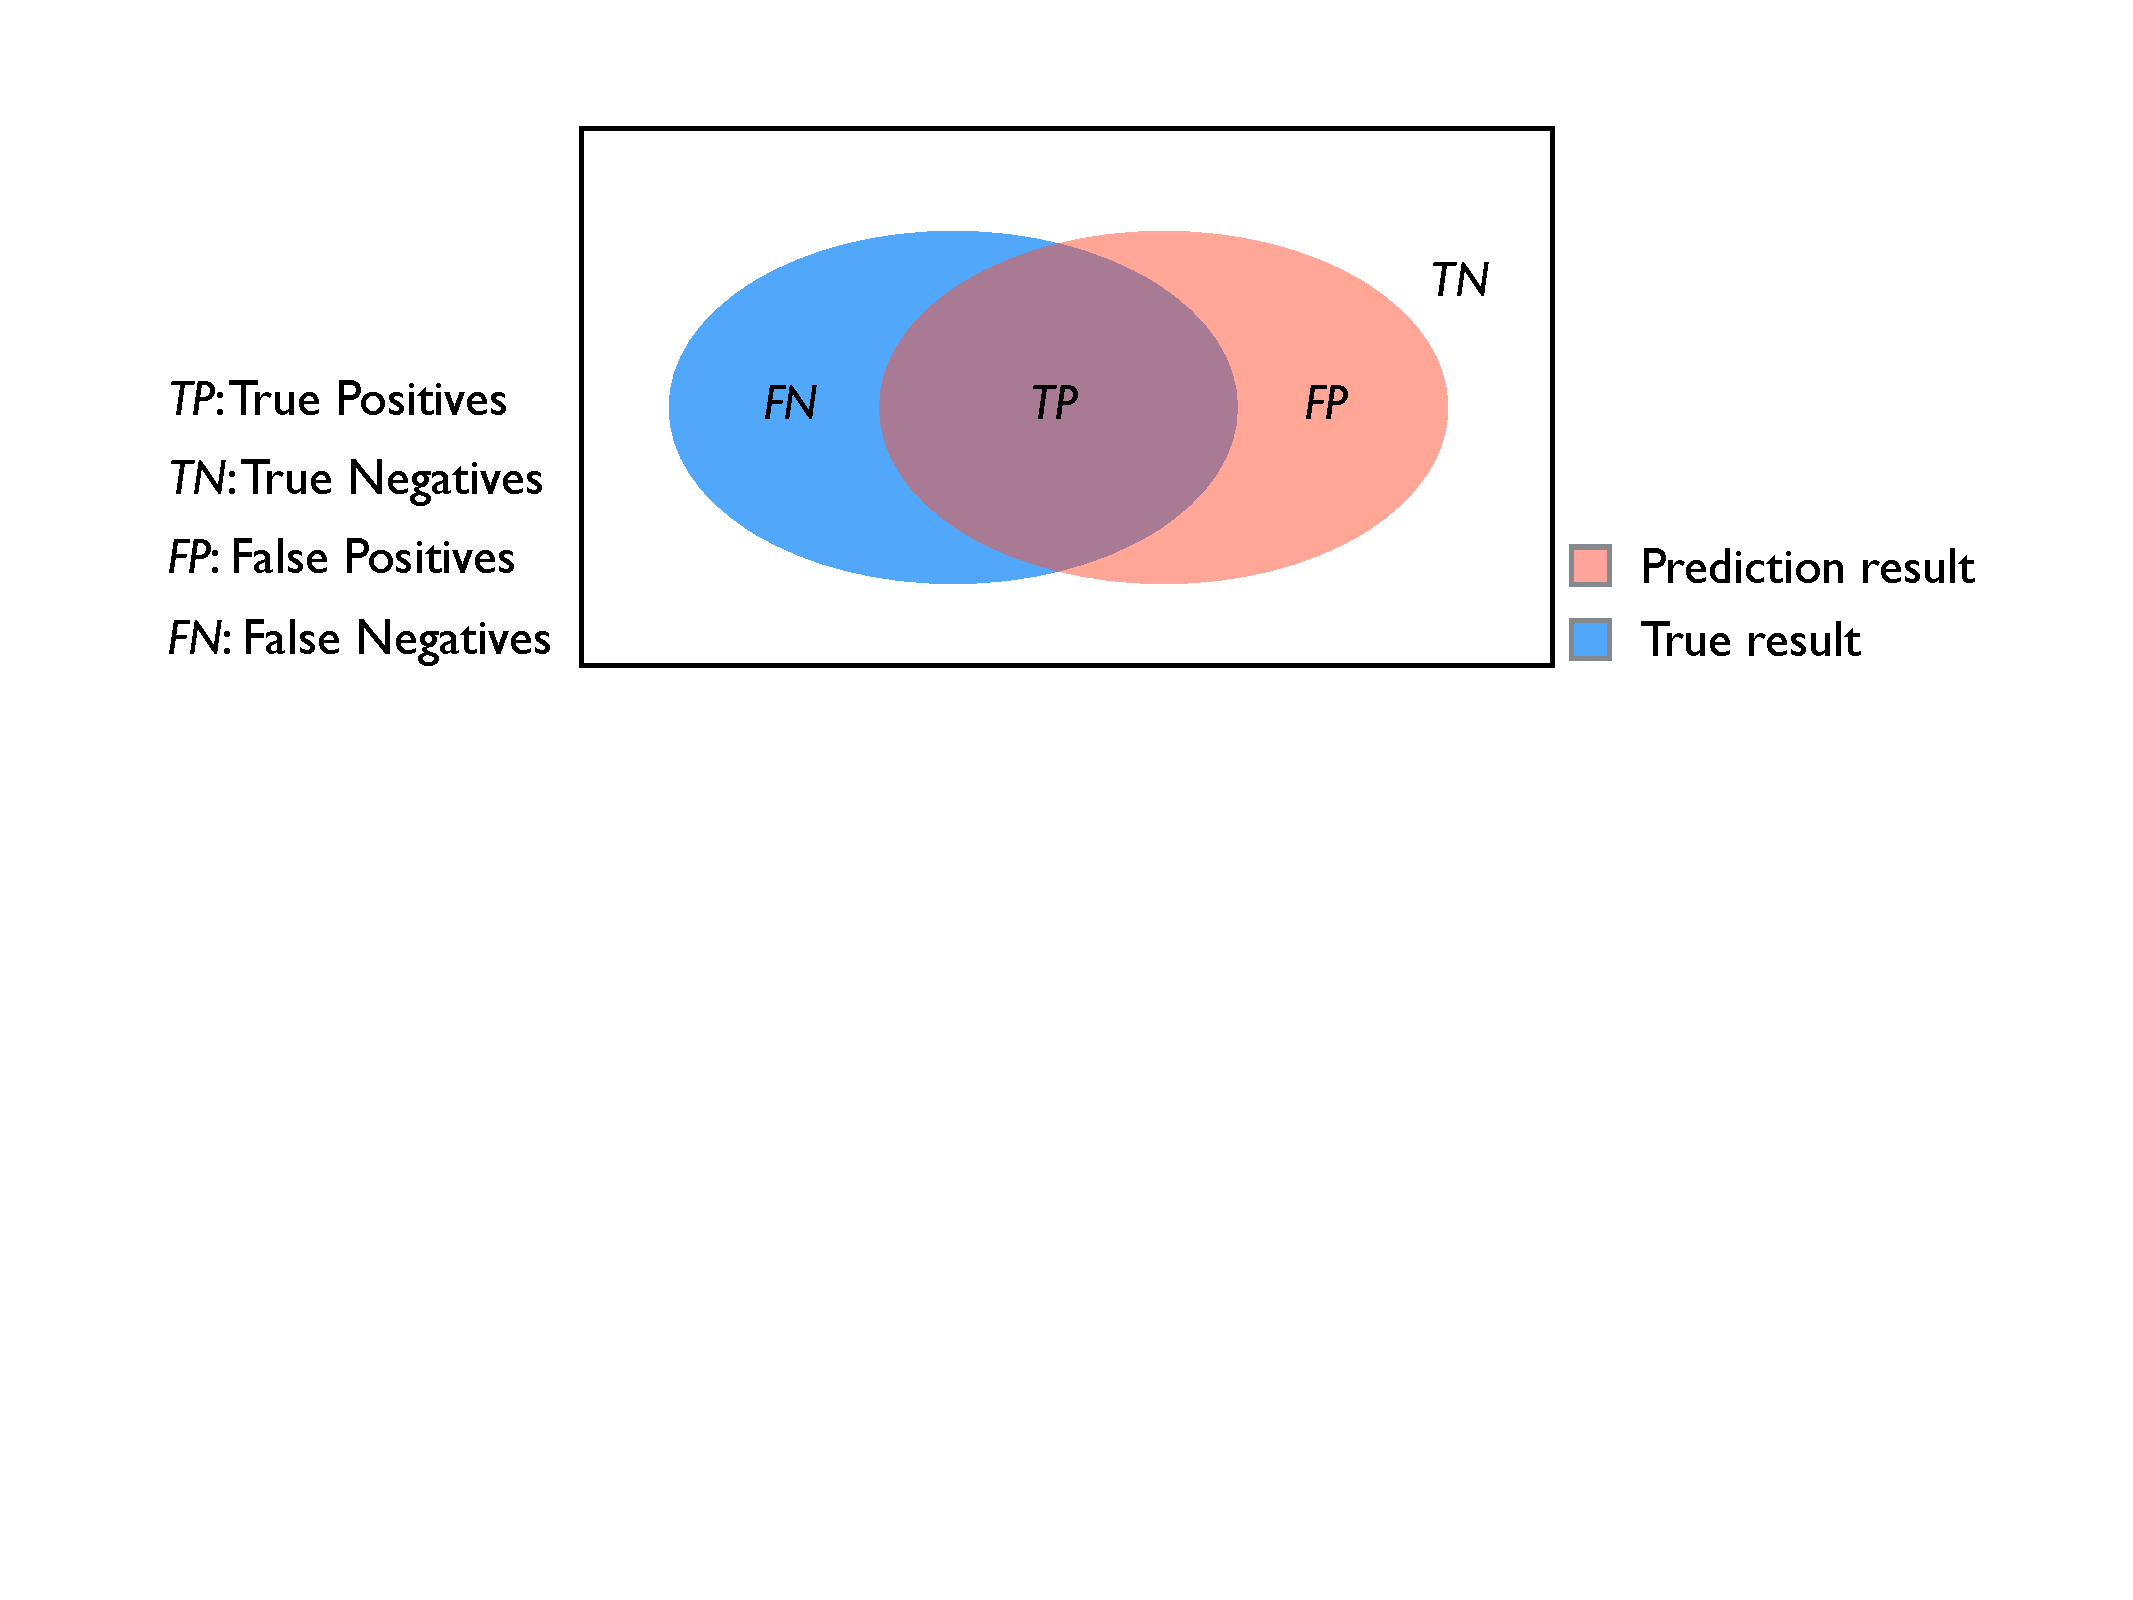
\includegraphics[width=0.9\textwidth]{../graphics/ModelEvaluation.pdf}
	\end{figure}
	\begin{itemize}
		\item Accuracy: the percentage of correctly classified samples.
		\begin{equation}
			\text{accuracy} = \frac{TP + TN}{TP + TN + FP + FN}
		\end{equation}
		\item The accuracy is the most widely used metric, but it does not tell us which kind of errors are made.
	\end{itemize}
\end{frame}

\begin{frame}{Model evaluation - Sensitivity / Recall}
	\begin{figure}[htb]
		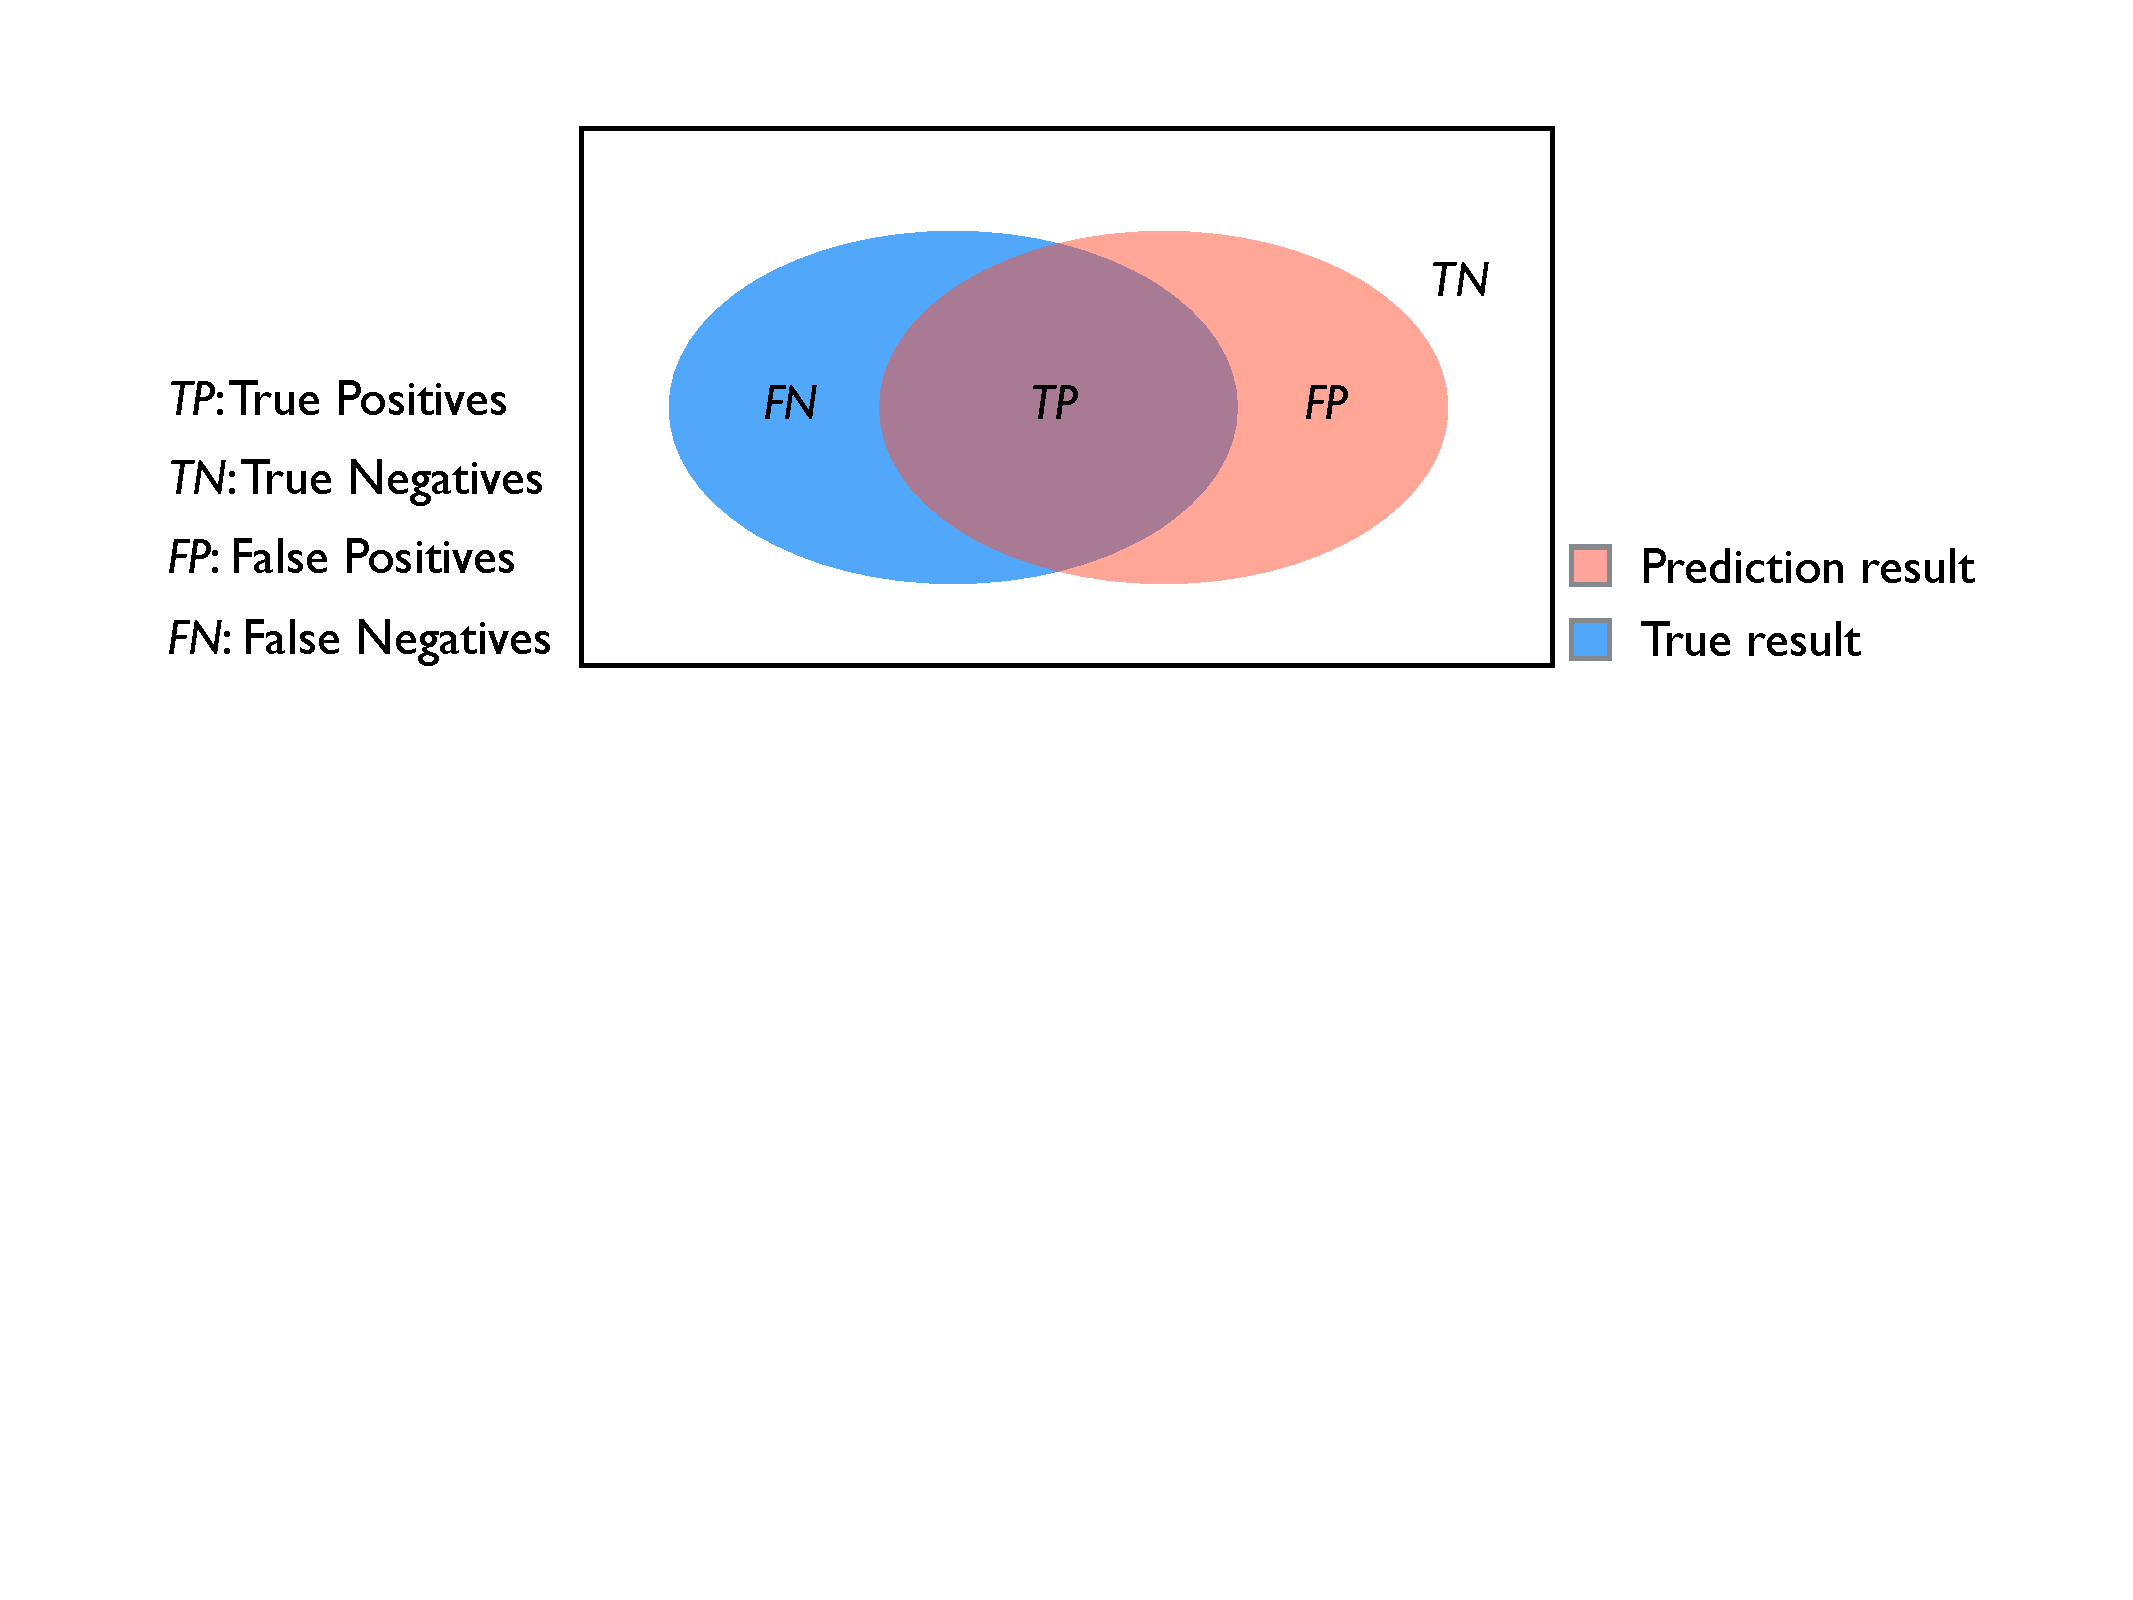
\includegraphics[width=0.9\textwidth]{../graphics/ModelEvaluation.pdf}
	\end{figure}
	\begin{itemize}
		\item Recall (aka sensitivity) is the percentage of positive samples that have been correctly classified as positive.
		\begin{equation}
			\text{recall} = \text{sensitivity} = \frac{TP}{TP + FN}
		\end{equation}
		\item Example: percentage of sick patients that are recognized as such by the diagnostic test.
		\item Sensitivity alone is useless, as if all all samples are classified positive, it will be $100\%$.
	\end{itemize}
\end{frame}

\begin{frame}{Model evaluation - Specificity}
	\begin{figure}[htb]
		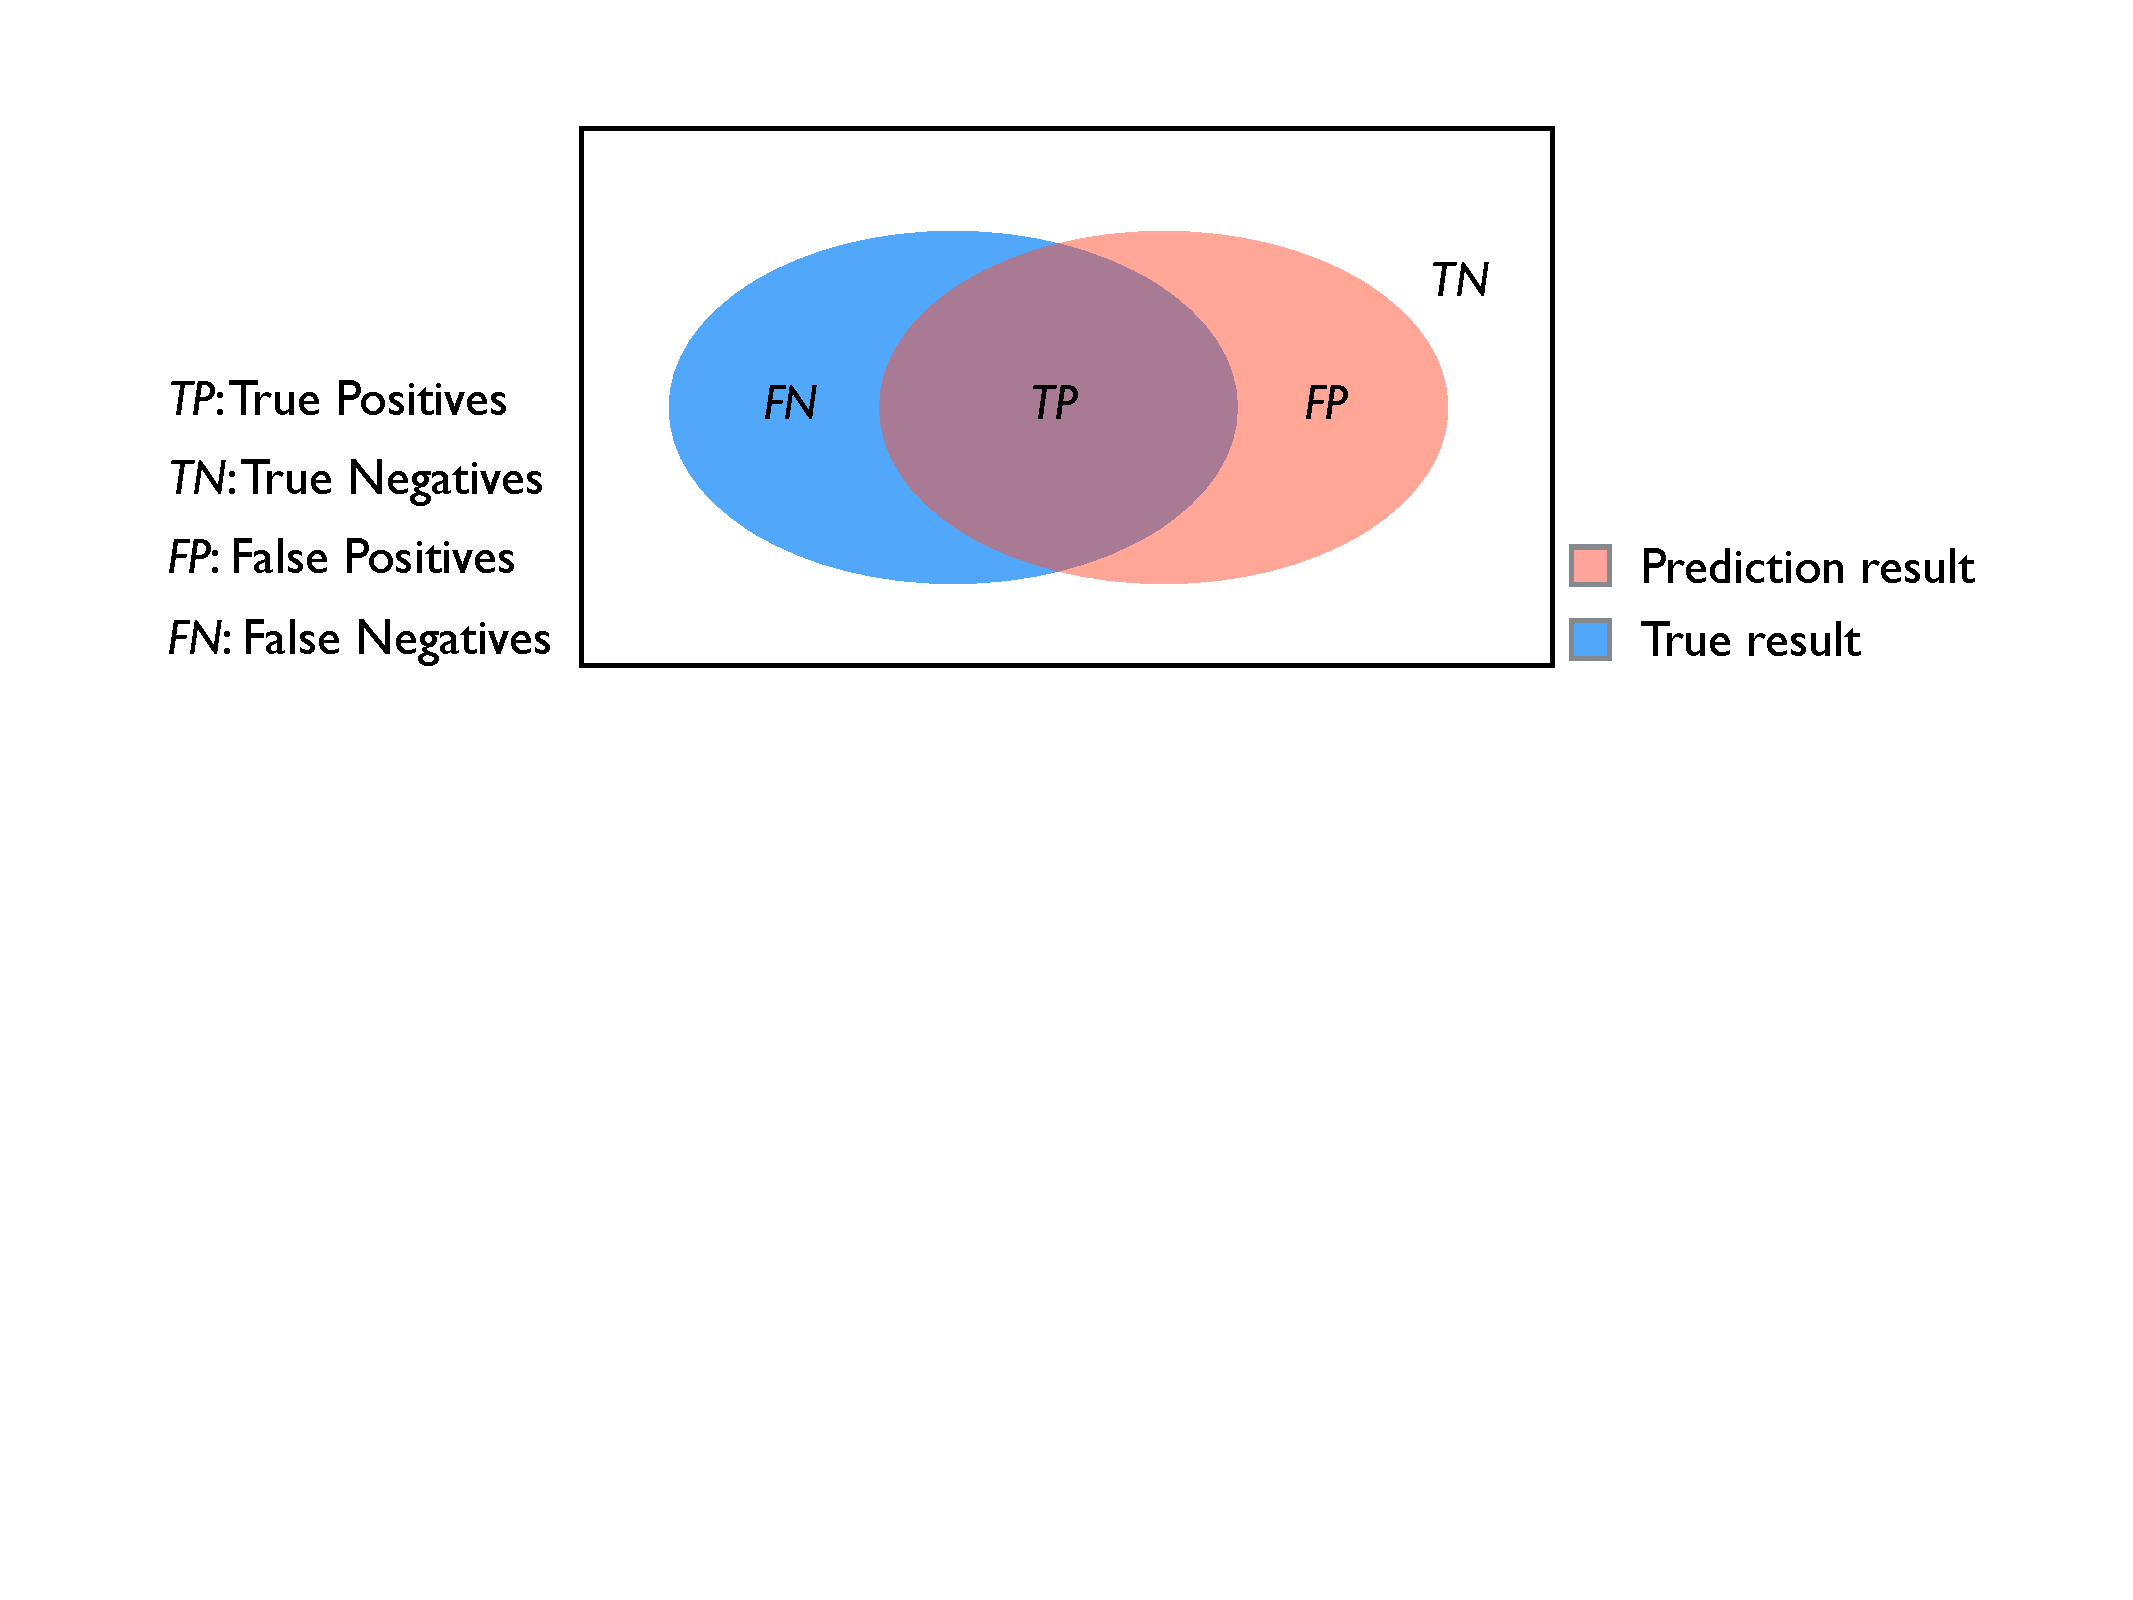
\includegraphics[width=0.9\textwidth]{../graphics/ModelEvaluation.pdf}
	\end{figure}
	\begin{itemize}
		\item Specificity is the percentage of negative samples that have been correctly classified as negatives
		\begin{equation}
			\text{specificity} = \frac{TN}{TN + FP}
		\end{equation}
		\item We usually seek a compromise between sensitivity and specificity.
		\item Specificity is not very informative if the dataset is very imbalanced.
	\end{itemize}
\end{frame}

%% \begin{frame}{Model evaluation - Precision / positive predictive value}
%% 	\begin{figure}[htb]
%% 		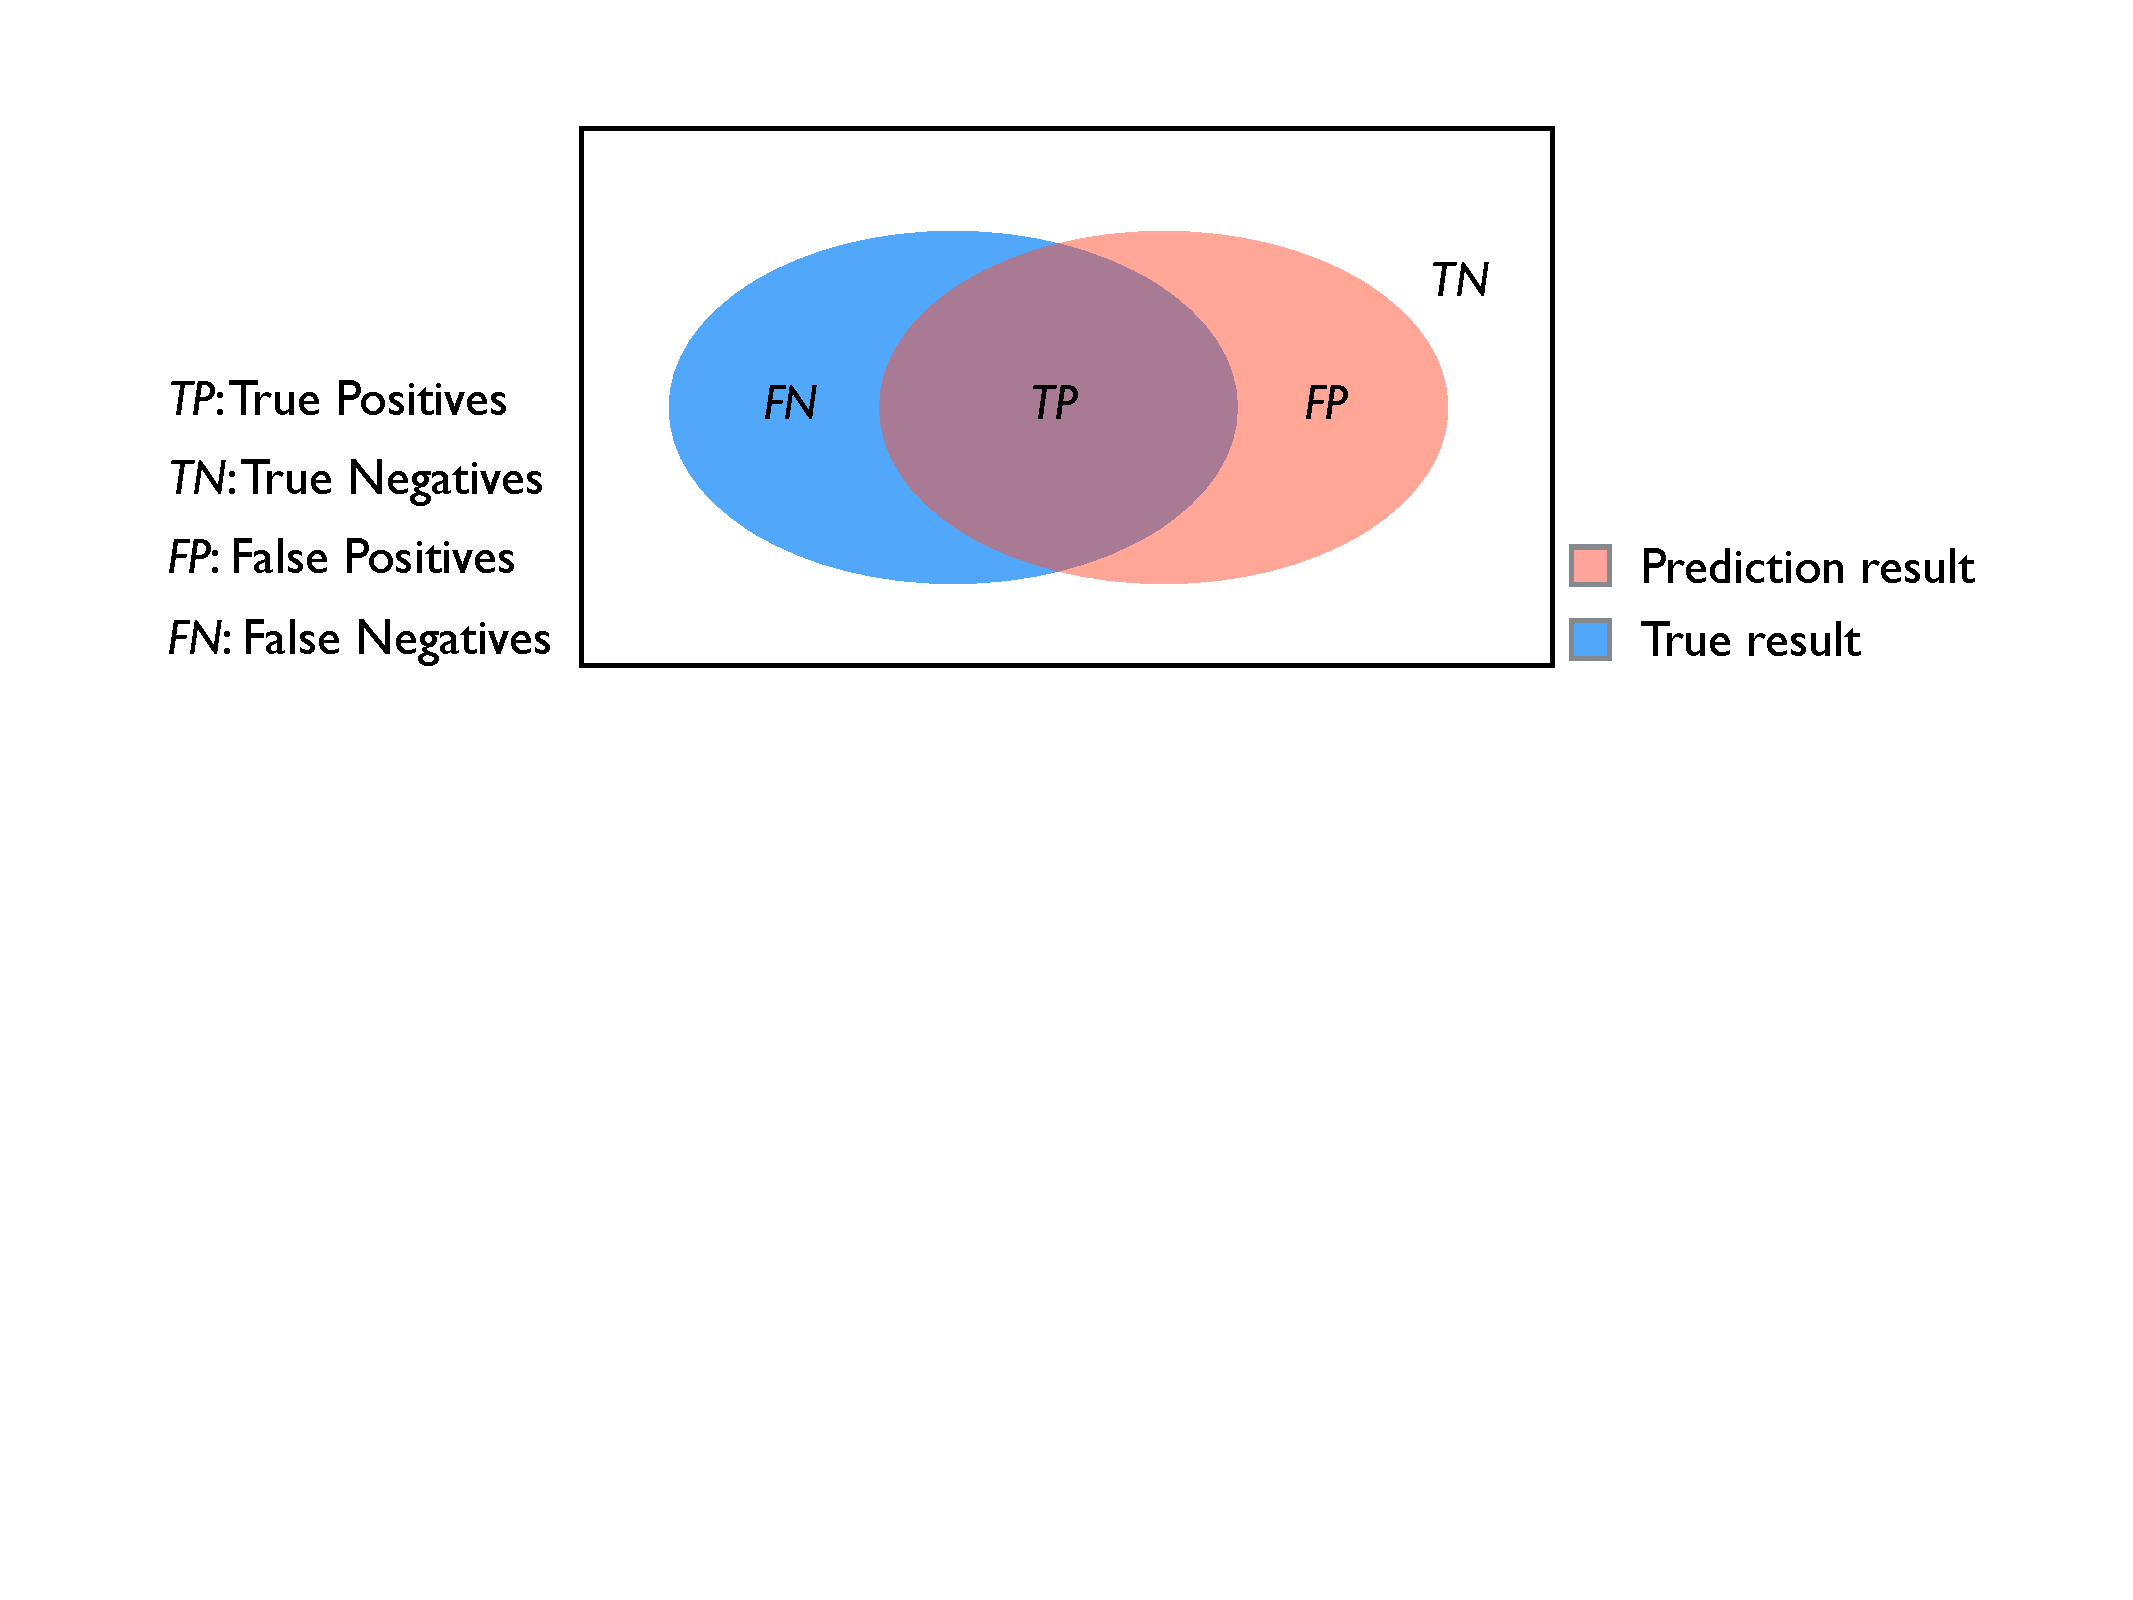
\includegraphics[width=0.9\textwidth]{../graphics/ModelEvaluation.pdf}
%% 	\end{figure}
%% 	\begin{itemize}
%% 		\item Precision (aka positive predictive value) is the probability that a sample is positive if it was classified positive.
%% 		\begin{equation}
%% 			\text{precision} = \frac{TP}{TP + FP}
%% 		\end{equation}
%% 		\item Example: precision gives you the probability of being sick, given that the diagnostic test was positive.
%% 		\item Precision is often preferred to specificity as it is also a suitable metric if the dataset is imbalanced.
%% 	\end{itemize}
%% \end{frame}

\begin{frame}{Model evaluation - Receiver Operating Characteristic (ROC)}
	\begin{figure}[htb]
		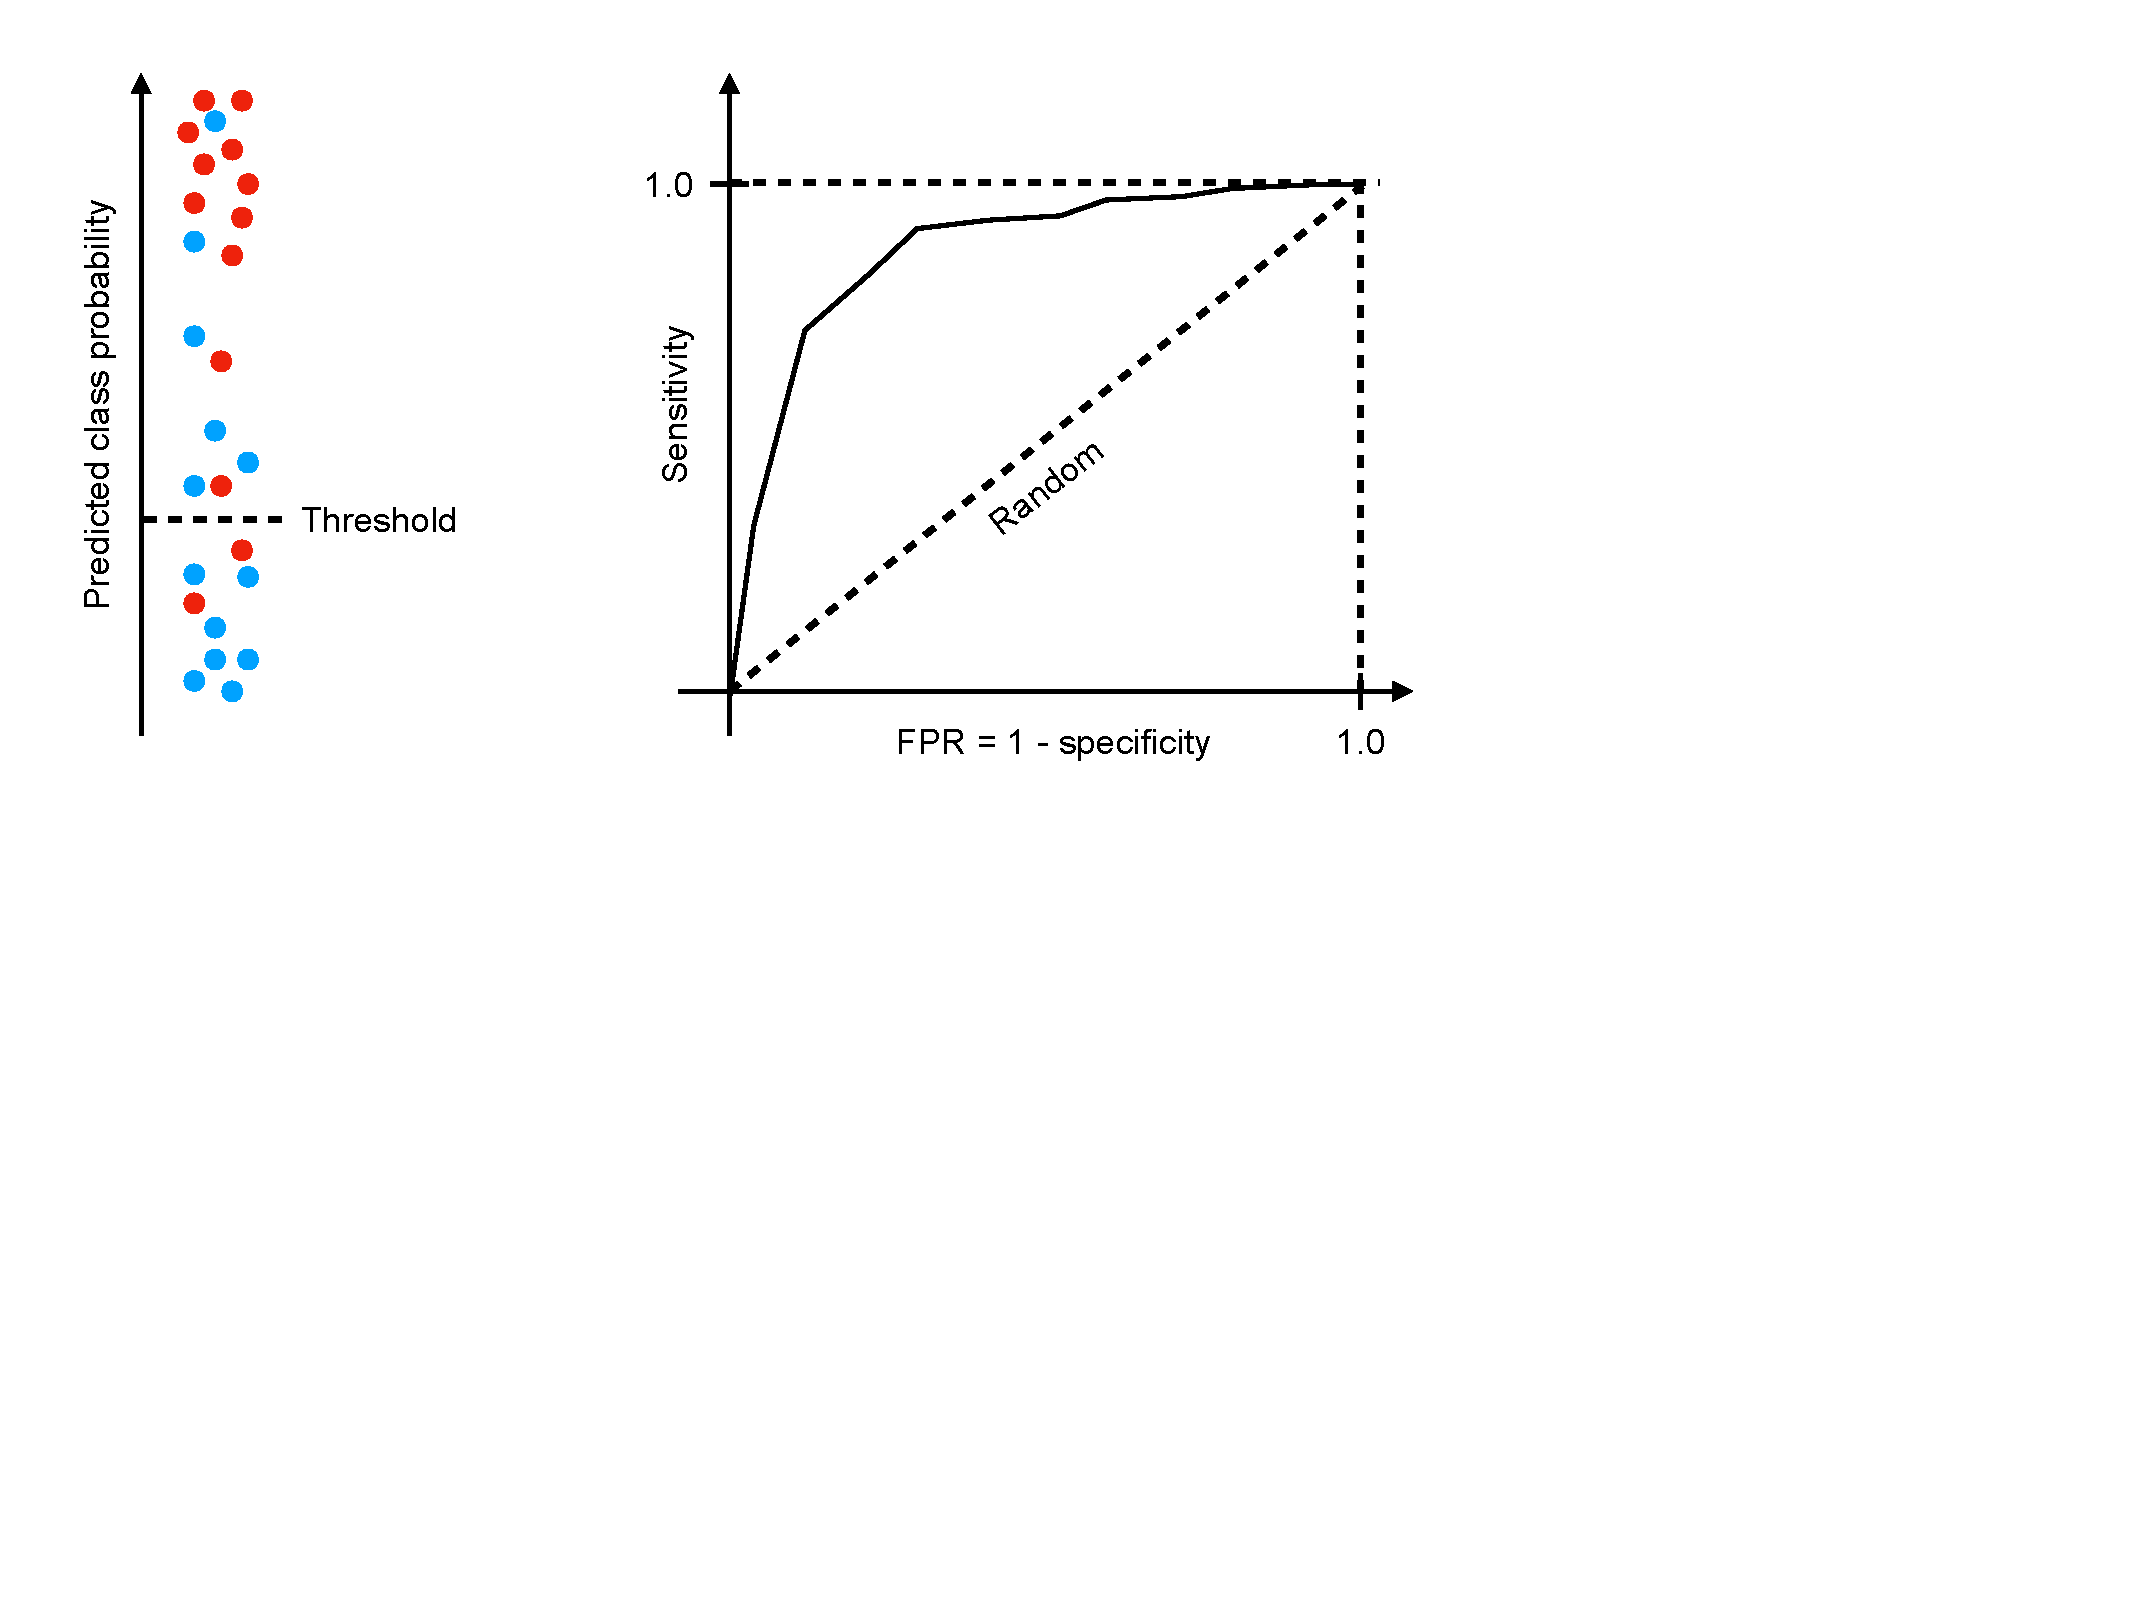
\includegraphics[width=0.65\textwidth]{../graphics/ROC.pdf}
	\end{figure}
	\begin{itemize}
		%% \item To measure a compromise between precision and recall, one can also use the $F_1$-score:
		%% \begin{equation}
		%% F_1 = 2 \frac{\text{precision} \times \text{recall}}{\text{precision} + \text{recall}}
		%% \end{equation}
	\item Another popular metric is related to $ROC$-curves (AUC: area under the curve).
		\item The AUC is identical to the concordance index: the probability that $(+,-)$ pairs of samples are correctly ordered.
	\end{itemize}
\end{frame}



\begin{frame}{Performance Assessment for a trained classifier}
	\begin{itemize}
		\item<1-> First idea: we train a classifier on the training set $T$ and calculate the accuracy on the same training set $T$ (empirical risk, training error).
		\item<2-> Problem: Training error is a poor approximation of the test error: a classifier might have good performance on the training set, but poor performance on the test set.
		\begin{figure}[htb]
			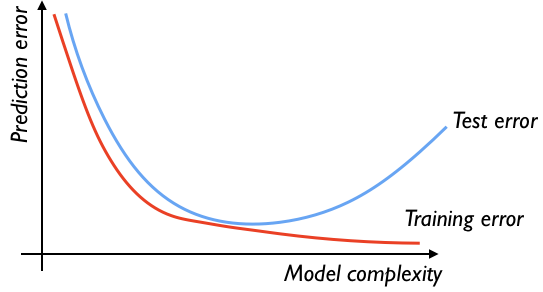
\includegraphics[width=0.6\textwidth]{../graphics/Training_and_test_error.png}
		\end{figure}
		\item<3-> We need to estimate the test error (error on unseen samples)!
	\end{itemize}
\end{frame}

\begin{frame}{Performance Assessment for a trained classifier}
	\begin{itemize}
		\item<1-> Second idea: to split the training set in two subsets $T_1$, $T_2$. We train on $T_1$, we test on $T_2$.
		\item<2-> Problem: annotated data is often expensive, and we would like to have the largest possible sets for training and testing.
		\item<3-> Third idea: Cross Validation. We split the data into $K$ folds. We train on $K-1$ folds, and we test on the remaining fold. We iterate until each fold has been used once for testing.
		\begin{figure}[htb]
			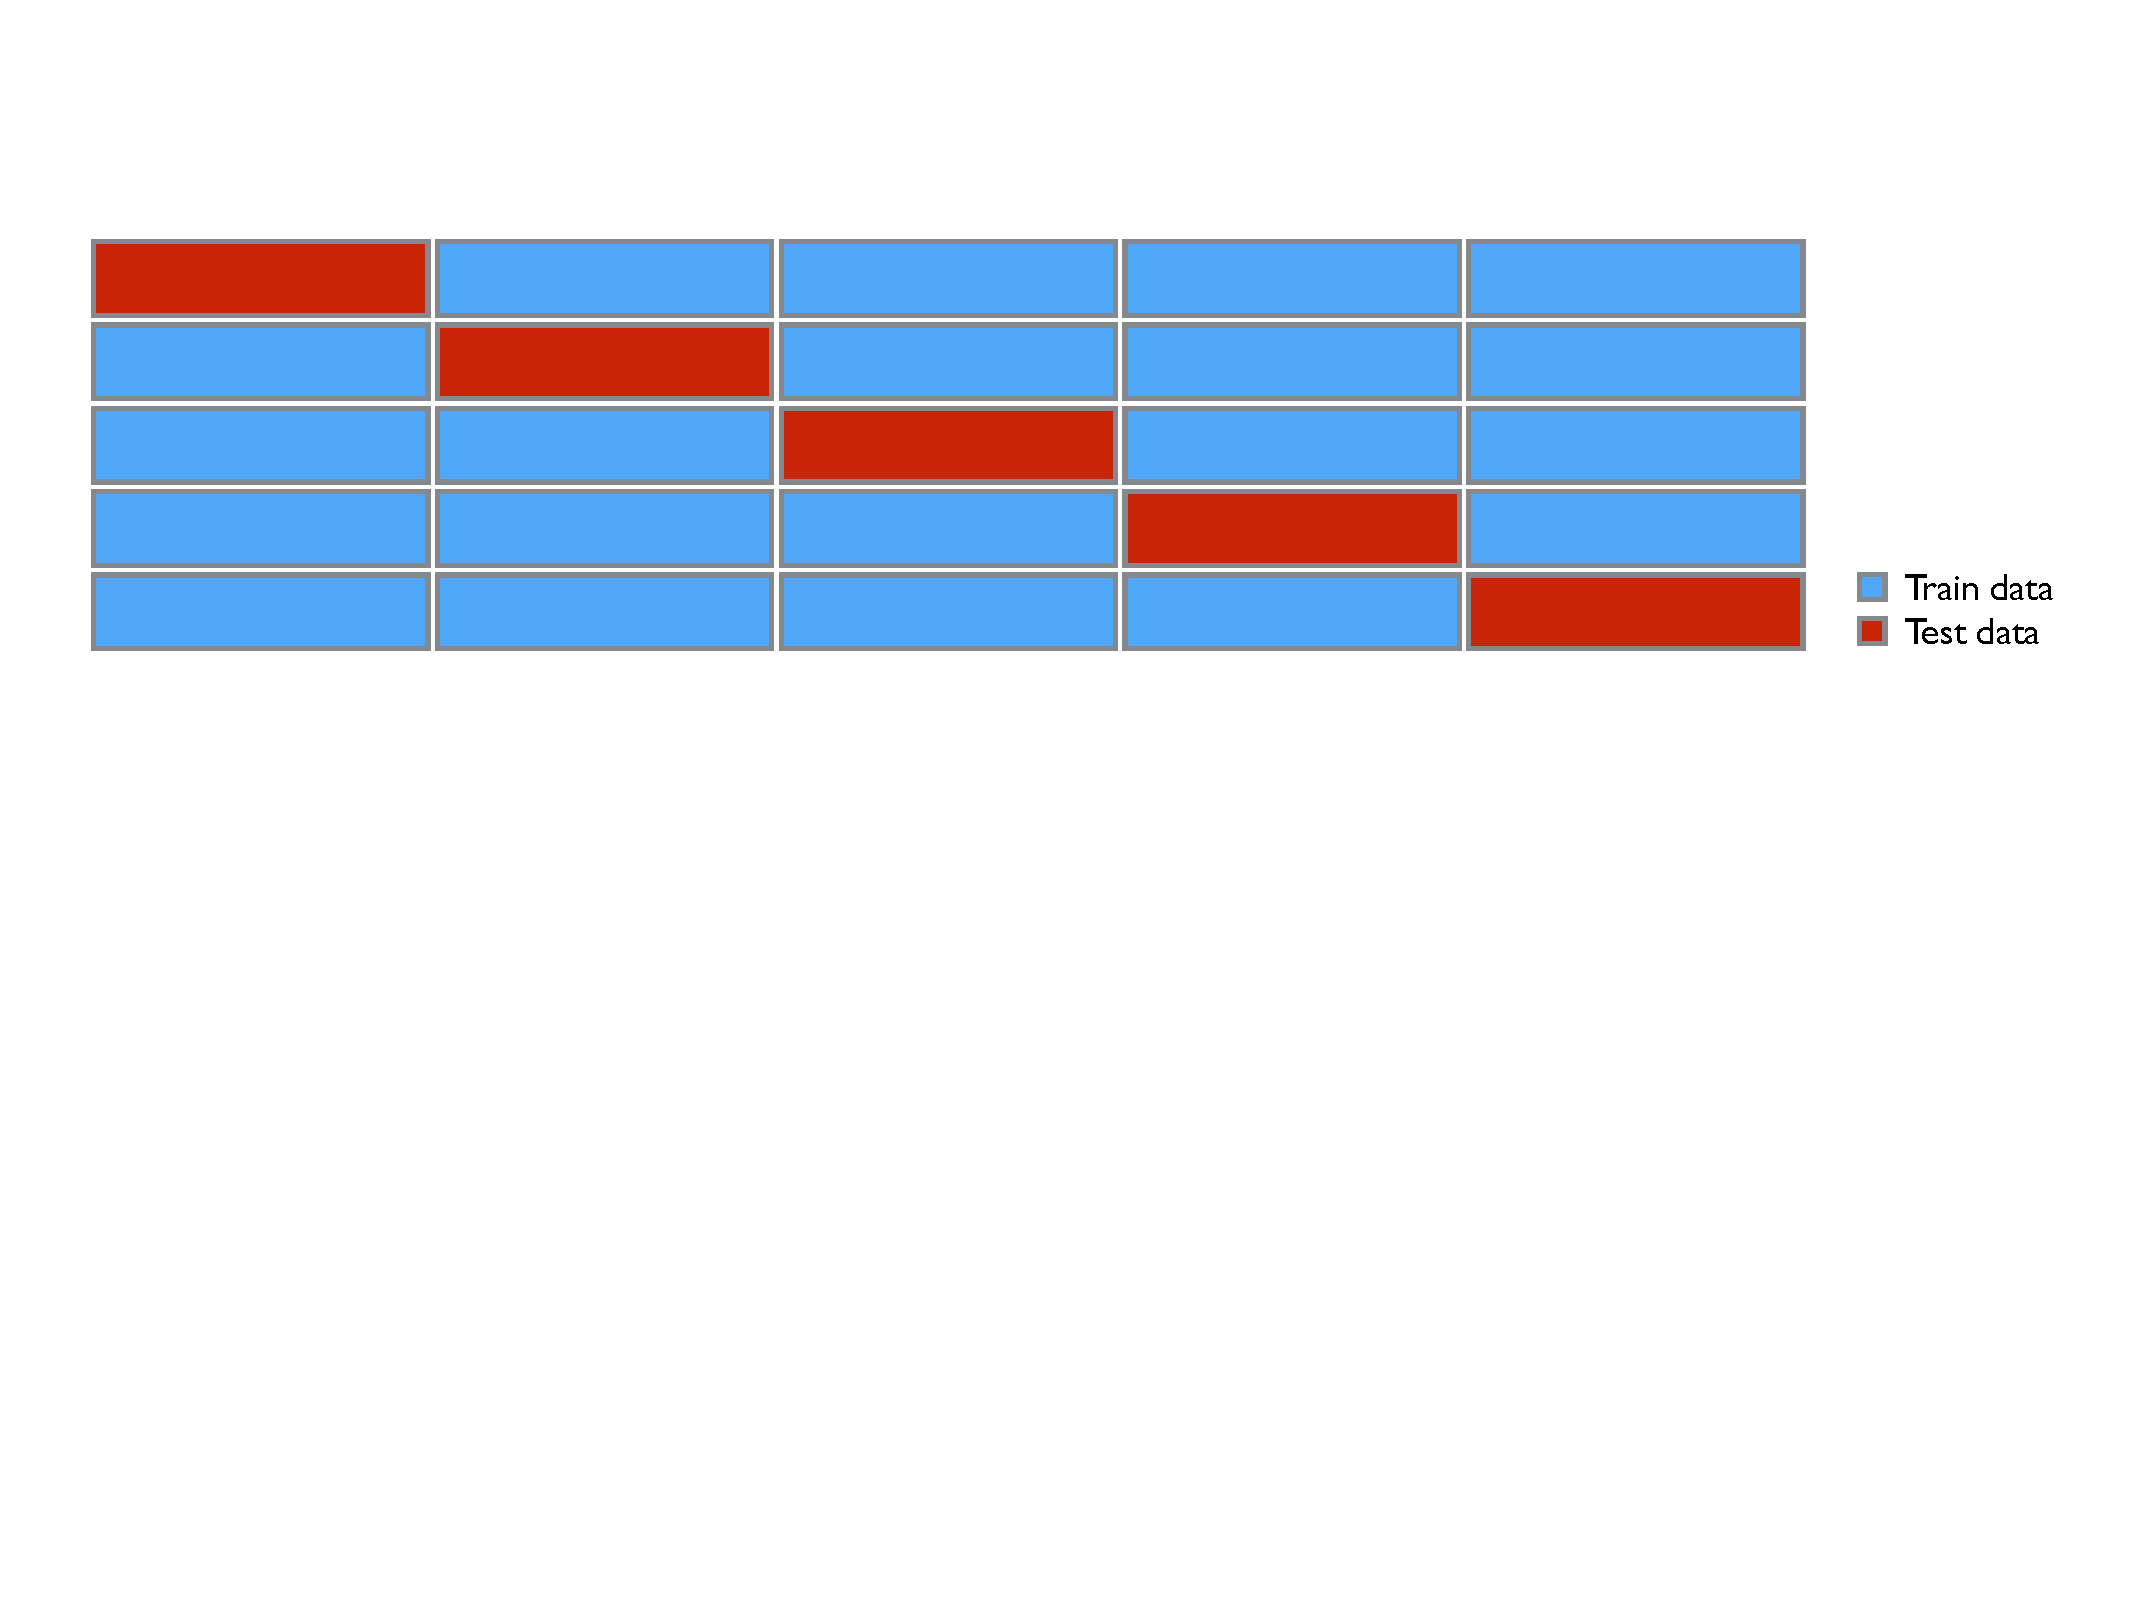
\includegraphics[width=0.65\textwidth]{../graphics/CV1.pdf}
		\end{figure}
		\item<4-> This provides us with an estimation of the accuracy for unseen data (test error).
%		\item<5-> Hyperparameter selection: we can now choose the hyperparameter with the best accuracy.
	\end{itemize}
\end{frame}

\begin{frame}{How to set hyperparameters ... }
	\begin{itemize}
		\item Training a classifier: finding automatically a large number of feature weights or other parameters from annotated data (in our example: coefficients of the polynomial).
		\item Hyperparameters: a small number of parameters that are set to control the training process, such as the regularization parameter $\lambda$.
		\item The question is: how can we find good hyperparameters?
		\item Strategy: grid search. We choose the set of hyperparameters that perform best (i.e. that lead to the classifier with the best performance).
	\end{itemize}
\end{frame}

% \begin{frame}{How to set hyperparameters: grid search}
% 	\begin{figure}[htb]
% 		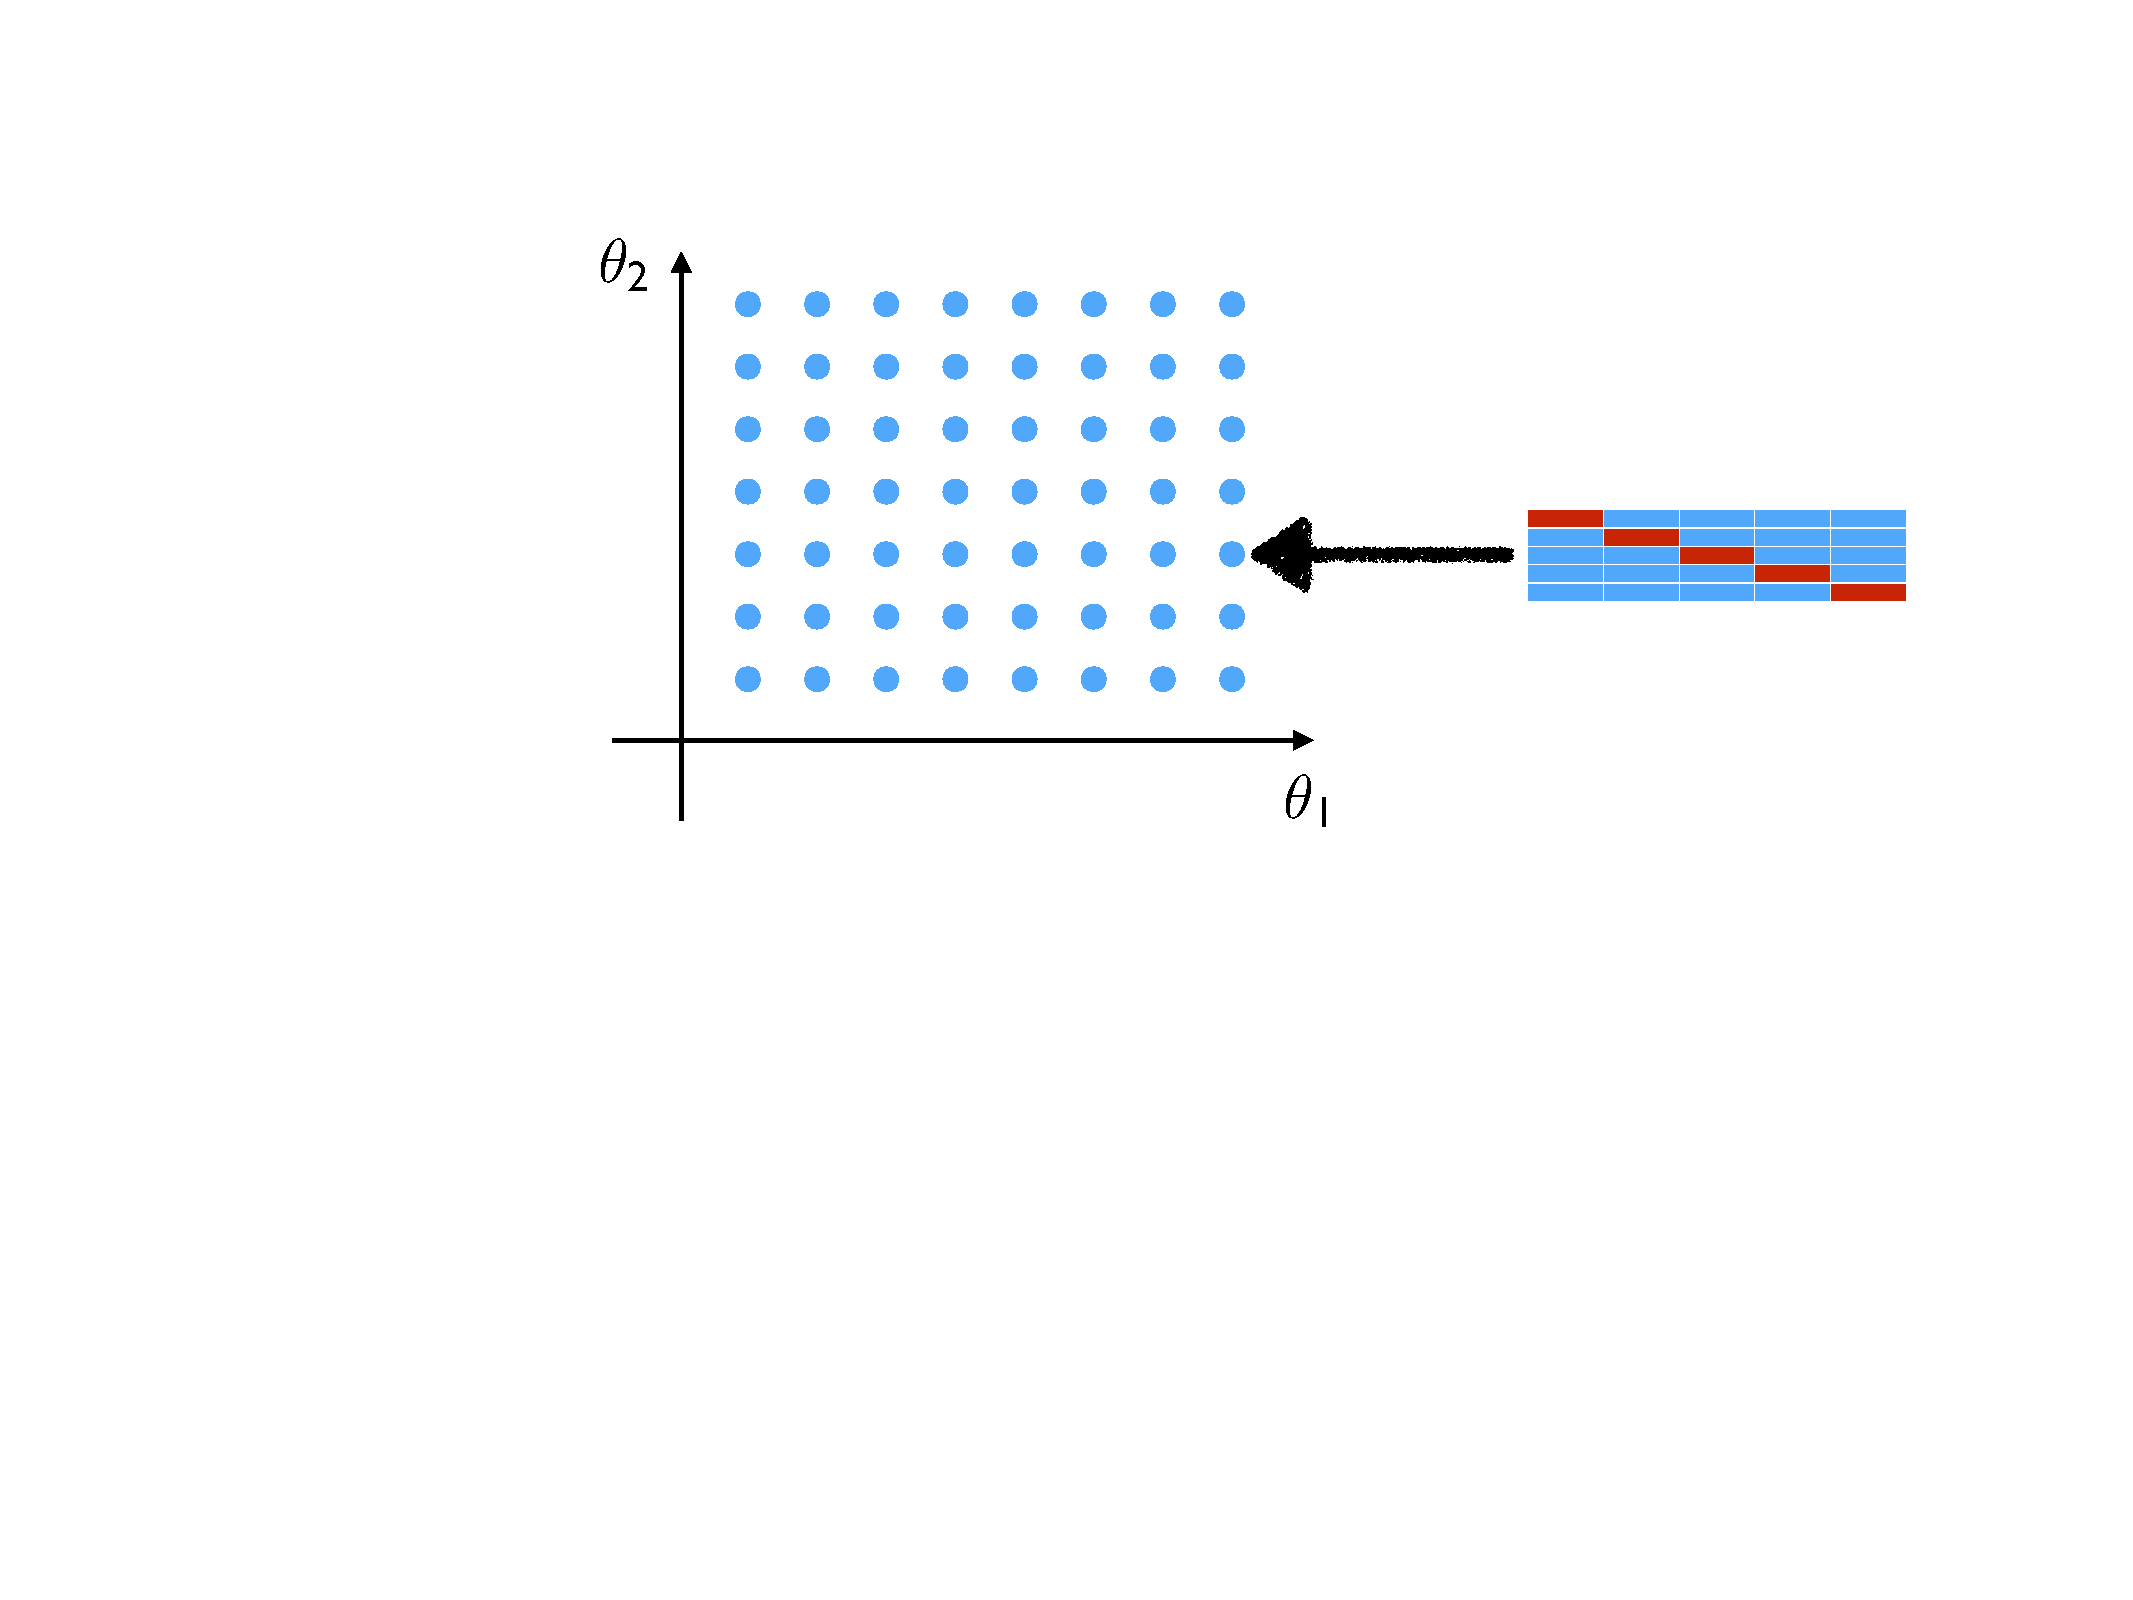
\includegraphics[width=0.8\textwidth]{../graphics/CV2.pdf}
% 	\end{figure}
% 	\begin{itemize}
% 		\item If there are several parameters, we can perform this for every combination of values (grid search).
% 		\item Alternatively, we can use random hyperparameter values.
% 		\item Problem: time-consuming.
% 		\item Ad hoc strategies to reduce the computation time: coarse-to-fine strategy.
% 	\end{itemize}
% \end{frame}

\begin{frame}{Performance evaluation with optimized hyperparameters}
	\begin{itemize}
		\item<1-> If we optimize the hyperparameters in this way, the final performance might be over-optimistic (we have chosen the hyperparameters that give best performance for the test set, i.e. we have used the test set to set the parameters).
		\item<2-> Solution: We split the training set in 3:
		\begin{itemize}
			\item {\bf Training set}: used to obtain the classifier for a given set of hyperparameters.
			\item {\bf Validation set}: used to find good hyperparameters.
			\item {\bf Test set}: used to evaluate performance.
		\end{itemize}
		\begin{figure}[htb]
			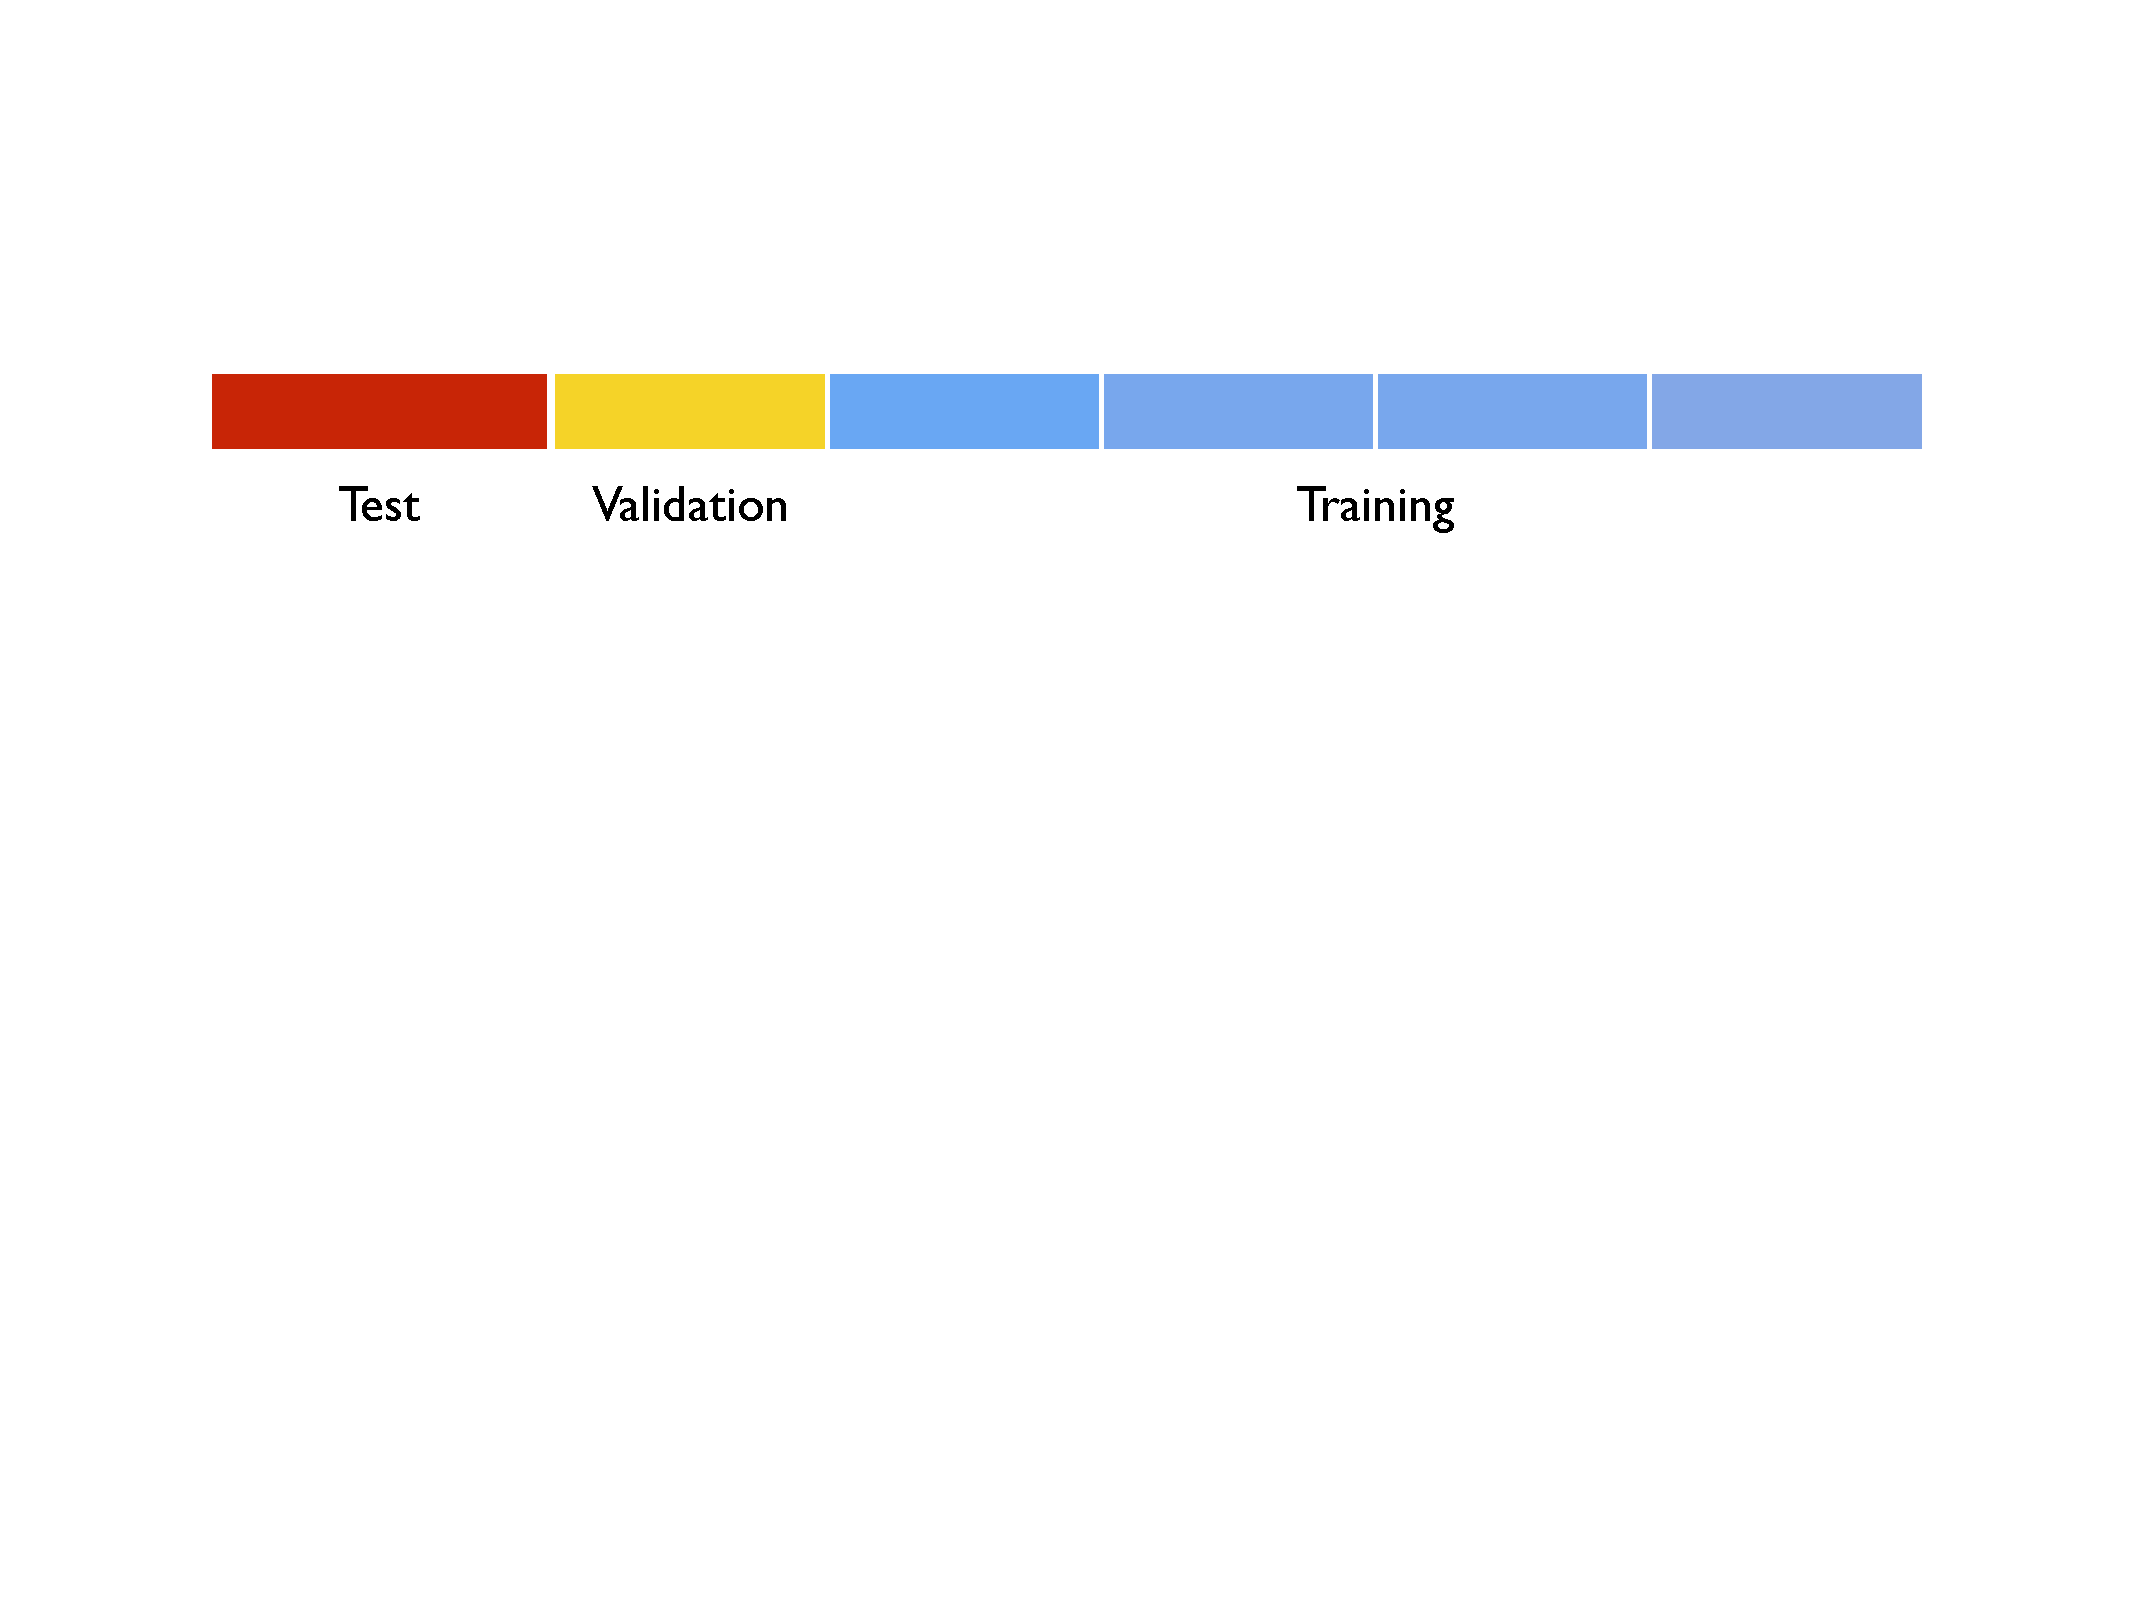
\includegraphics[width=0.9\textwidth]{../graphics/CV3_single.pdf}
		\end{figure}
	\end{itemize}
\end{frame}

%% \begin{frame}{Performance evaluation in deep learning}
%% 	\begin{itemize}
%% 		\item<1-> If we want to use make of the entire training set, we will perform nested cross validation:
%%  		\begin{figure}[htb]
%%  			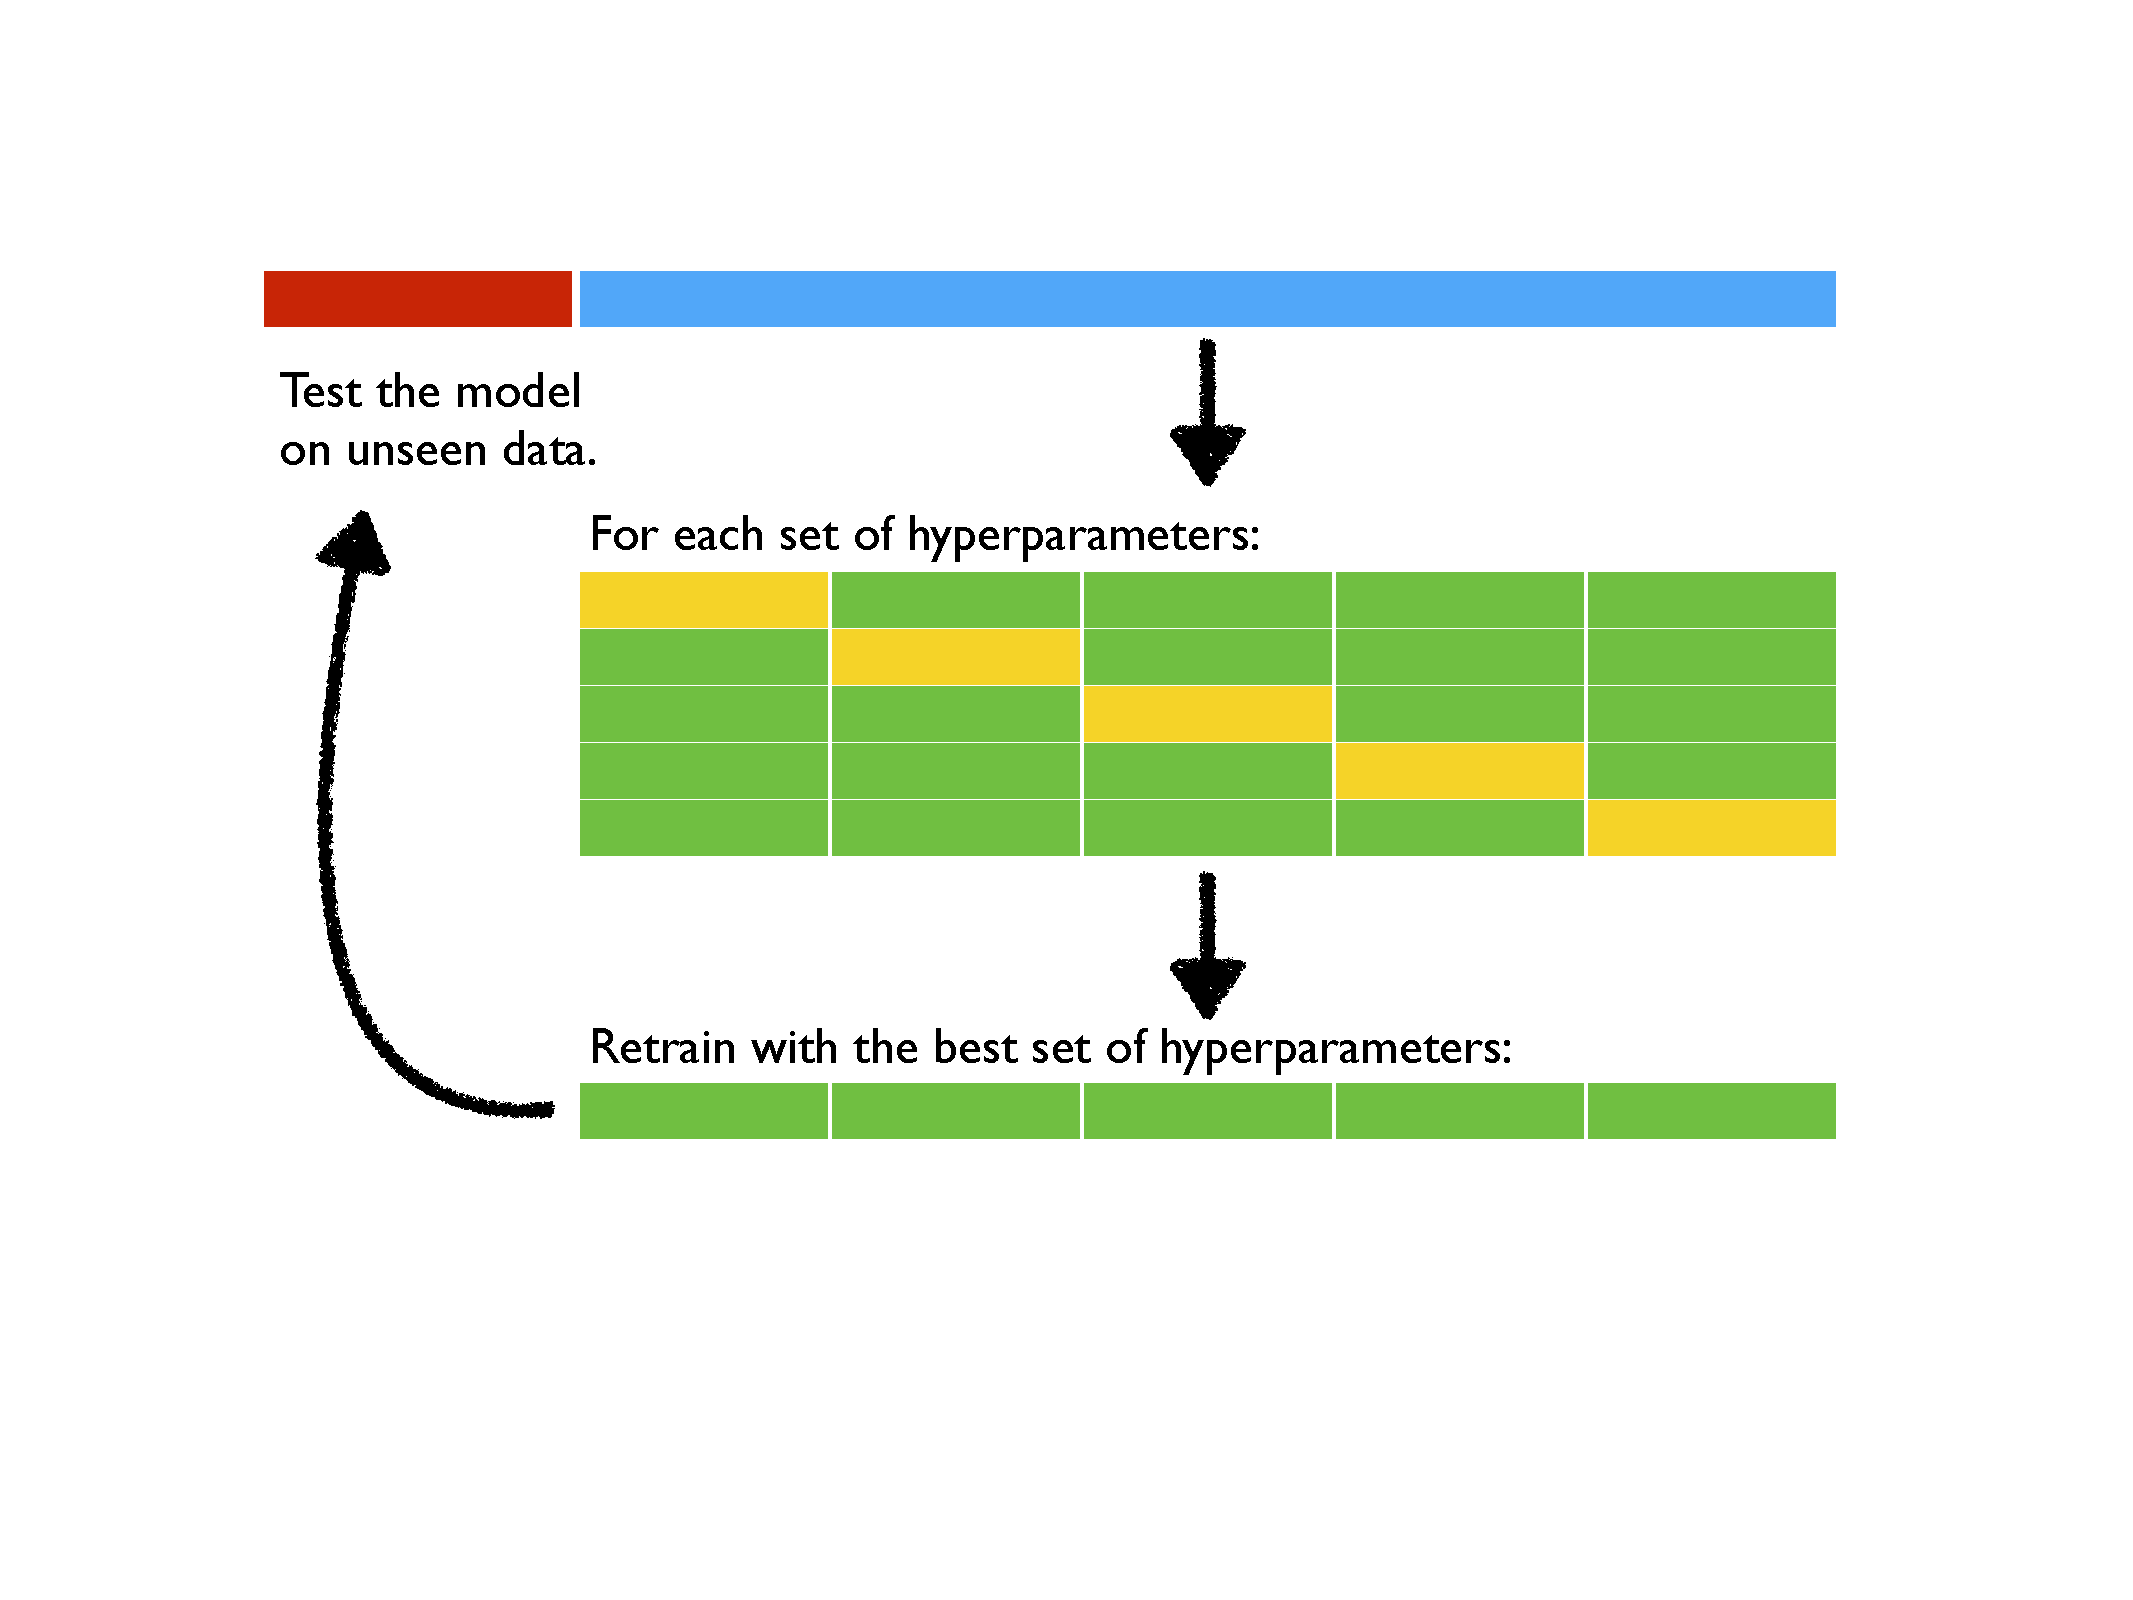
\includegraphics[width=0.8\textwidth]{../graphics/NestedCrossValidation.pdf}
%%  		\end{figure}
%% 		\item<2-> Nested cross validation is extremely time consuming.
%% 		\item<3-> In the context of deep learning with long training times, nested cross validation is rarely used.
%% 	\end{itemize}
%% \end{frame}



%%%%%%%%%%%%%%%%%%%%%%%%%%%%%%%%%%%%%%%%%%%%%%%%%%%%%%%%%%%%%%%%%%%%%%%%%
%%%%%%%%%%%%%%%%%%%%%%%%%%%%%%%%%%%%%%%%%%%%%%%%%%%%%%%%%%%%%%%%%%%%%%%%%
\section{Supervised Learning: Example algorithms}
\frame{\frametitle{Overview}\tableofcontents[currentsection]}

% \begin{frame}{Linear Discriminant Analysis (LDA)}
% \begin{figure}[htb]
% 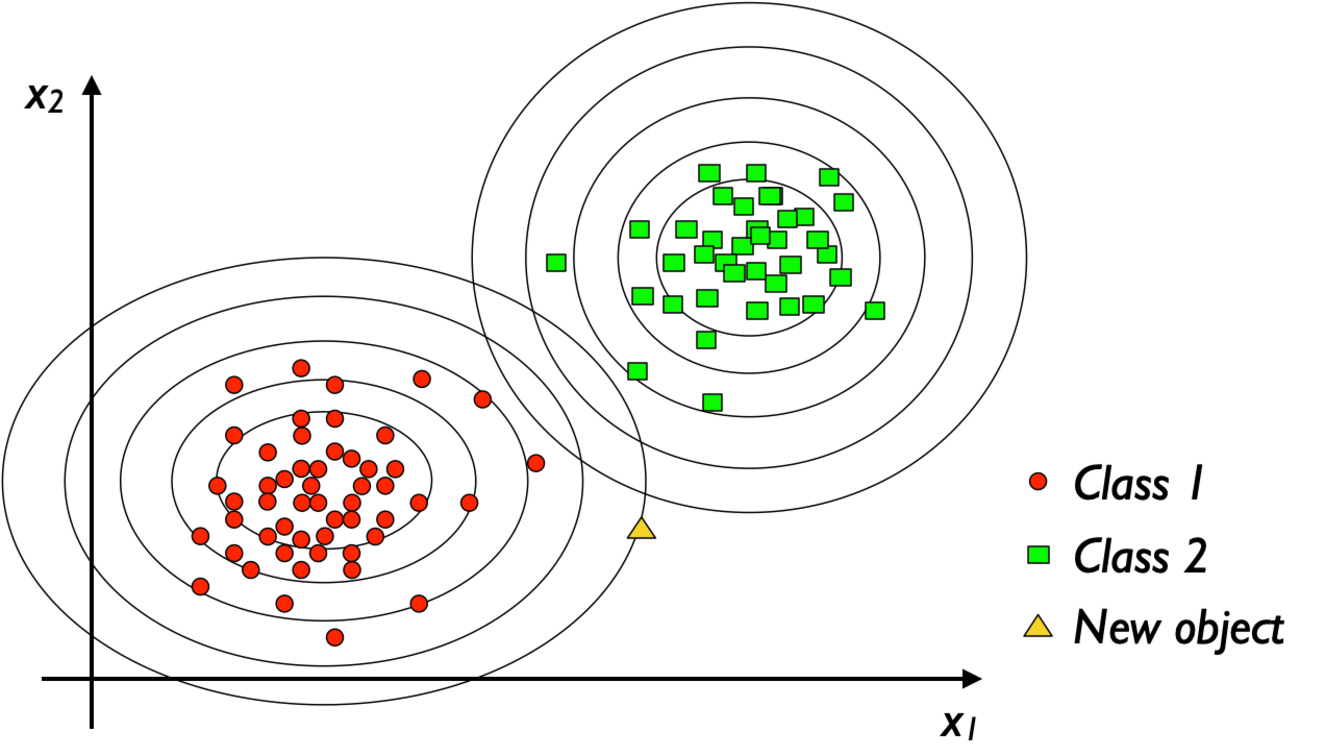
\includegraphics[width=0.65\textwidth]{../graphics/LDA3.pdf}
% \end{figure}
% \begin{itemize}
% \item We estimate the class dependent feature densities $p(x|y=k)$.
% \item We then find the class that maximises the posterior probability:
% \begin{equation*}
% \hat{y}(x) = \arg\max_k P(y=k \, | \, x) = \arg\max_k p(x\,|\,y=k)P(y=k)
% \end{equation*}
% \item If we assume normal distributions, we can infer a linear decision rule.
% \end{itemize}\end{frame}

% \begin{frame}{Support Vector Machines}
% 	\begin{figure}[htb]
% 		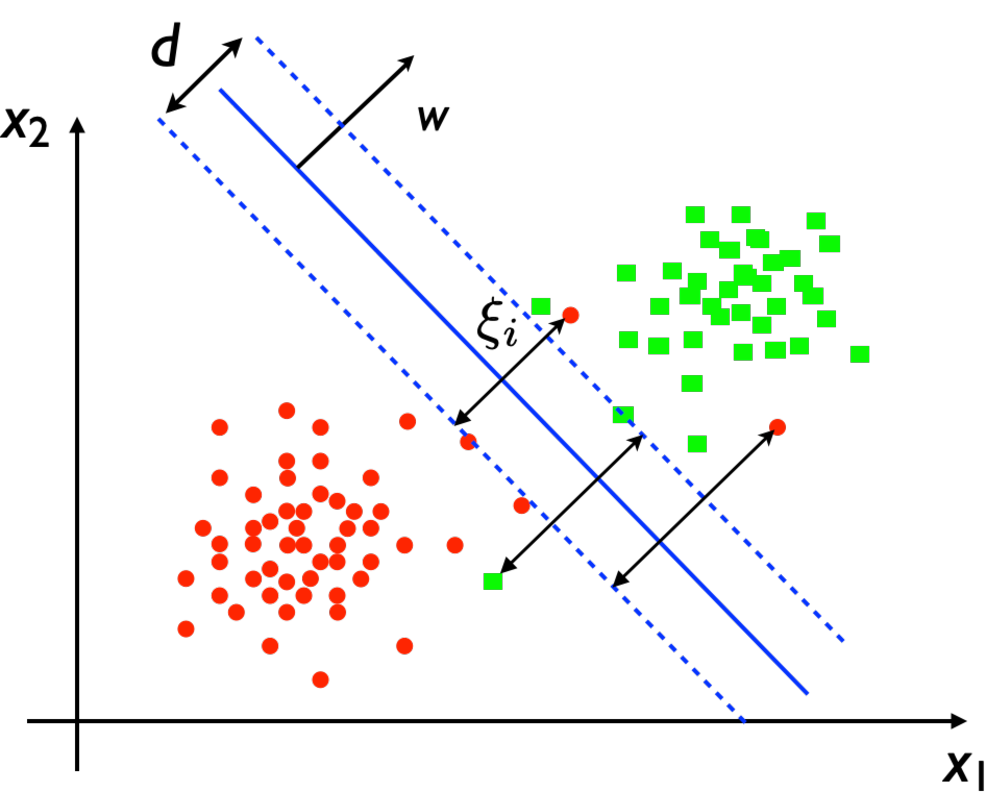
\includegraphics[width=0.45\textwidth]{../graphics/SVM_nonsep.pdf}
% 	\end{figure}
% 	\begin{itemize}
% 		\item Instead of simply placing a single line, we can also place a “ribbon”, i.e. two parallel lines separated by a distance $d$, which we try to maximize.
% 		\item Support Vector Machines can be written as a convex optimization problem under constraints:
% 		\begin{equation*}
% 			\min_{w,\xi} \|w\|^2 + C \sum_{i=1}^{N}\xi_i
% 		\end{equation*}
% 	\end{itemize}
% \end{frame}

% \begin{frame}{Random Forest: Decision trees}
% \begin{figure}[htb]
% 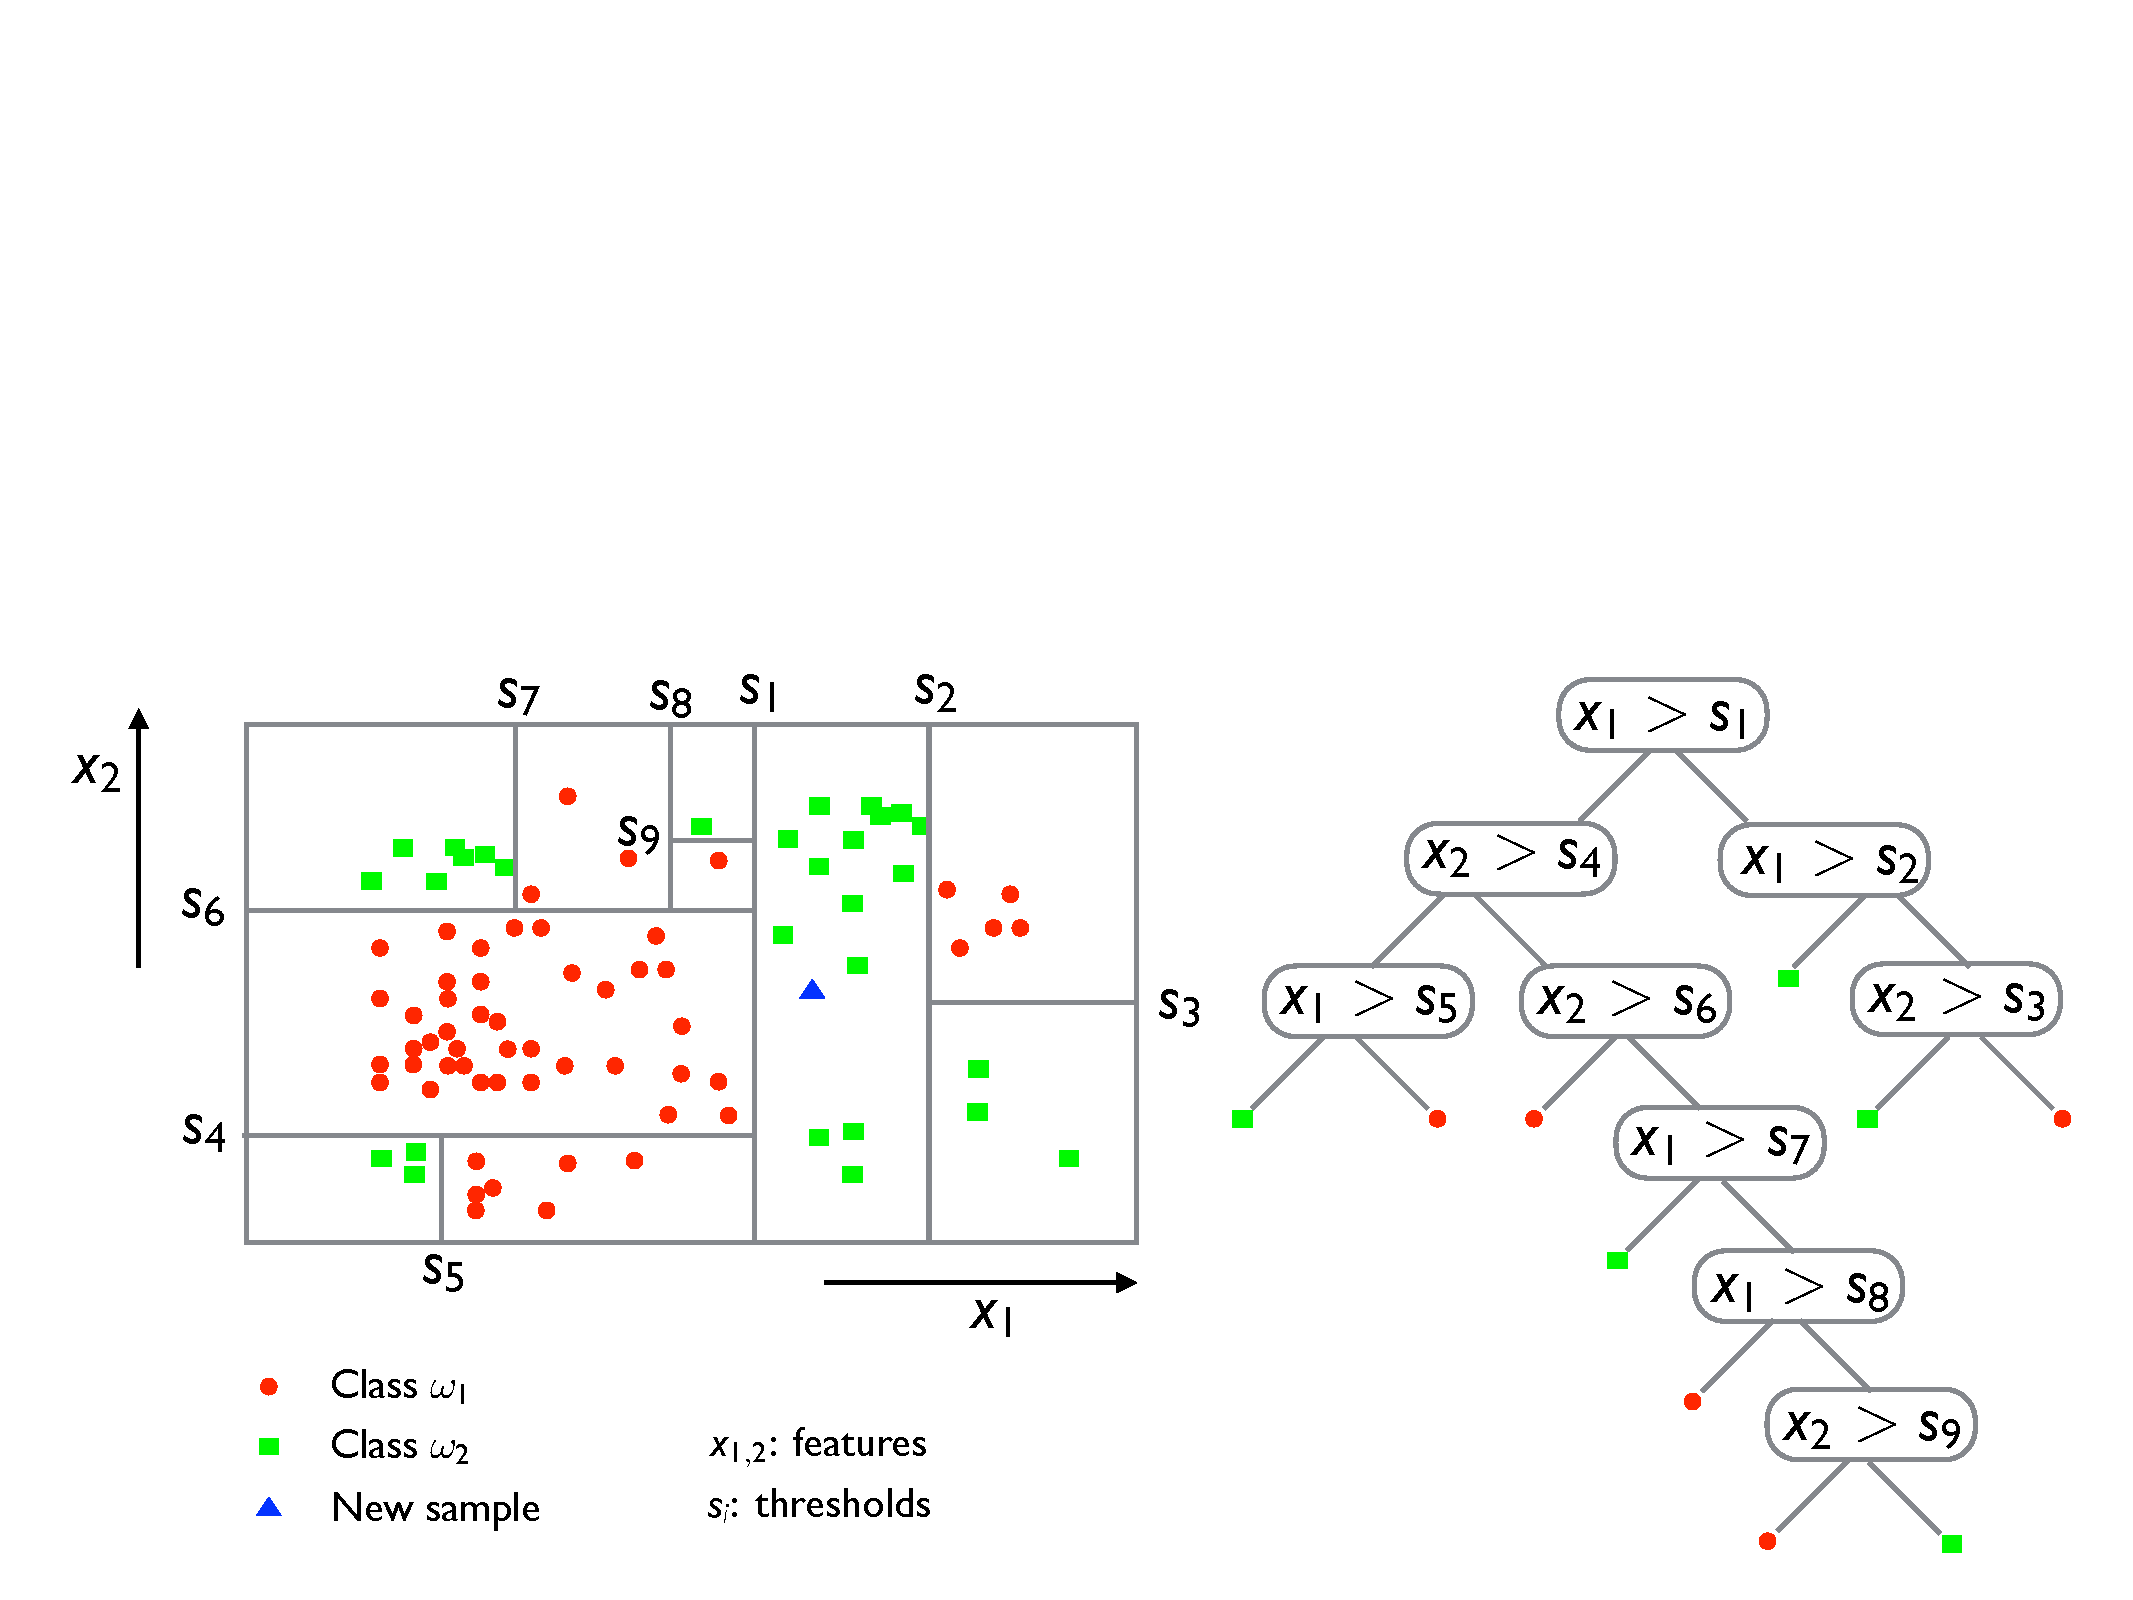
\includegraphics[width=0.8\textwidth]{../graphics/RF2.pdf}
% \end{figure}
% \begin{itemize}
% 	\item Decision trees correspond to a series of binary decisions that partition the feature space.
% 	\item Classification of a new object: application of the binary decision rules and assignment of the leaf label.
% 	\item The decision boundaries can be very complex and adapt very tightly to the training set.
% \end{itemize}
% \end{frame}

% \begin{frame}{Random Forests}
% \begin{figure}[htb]
% 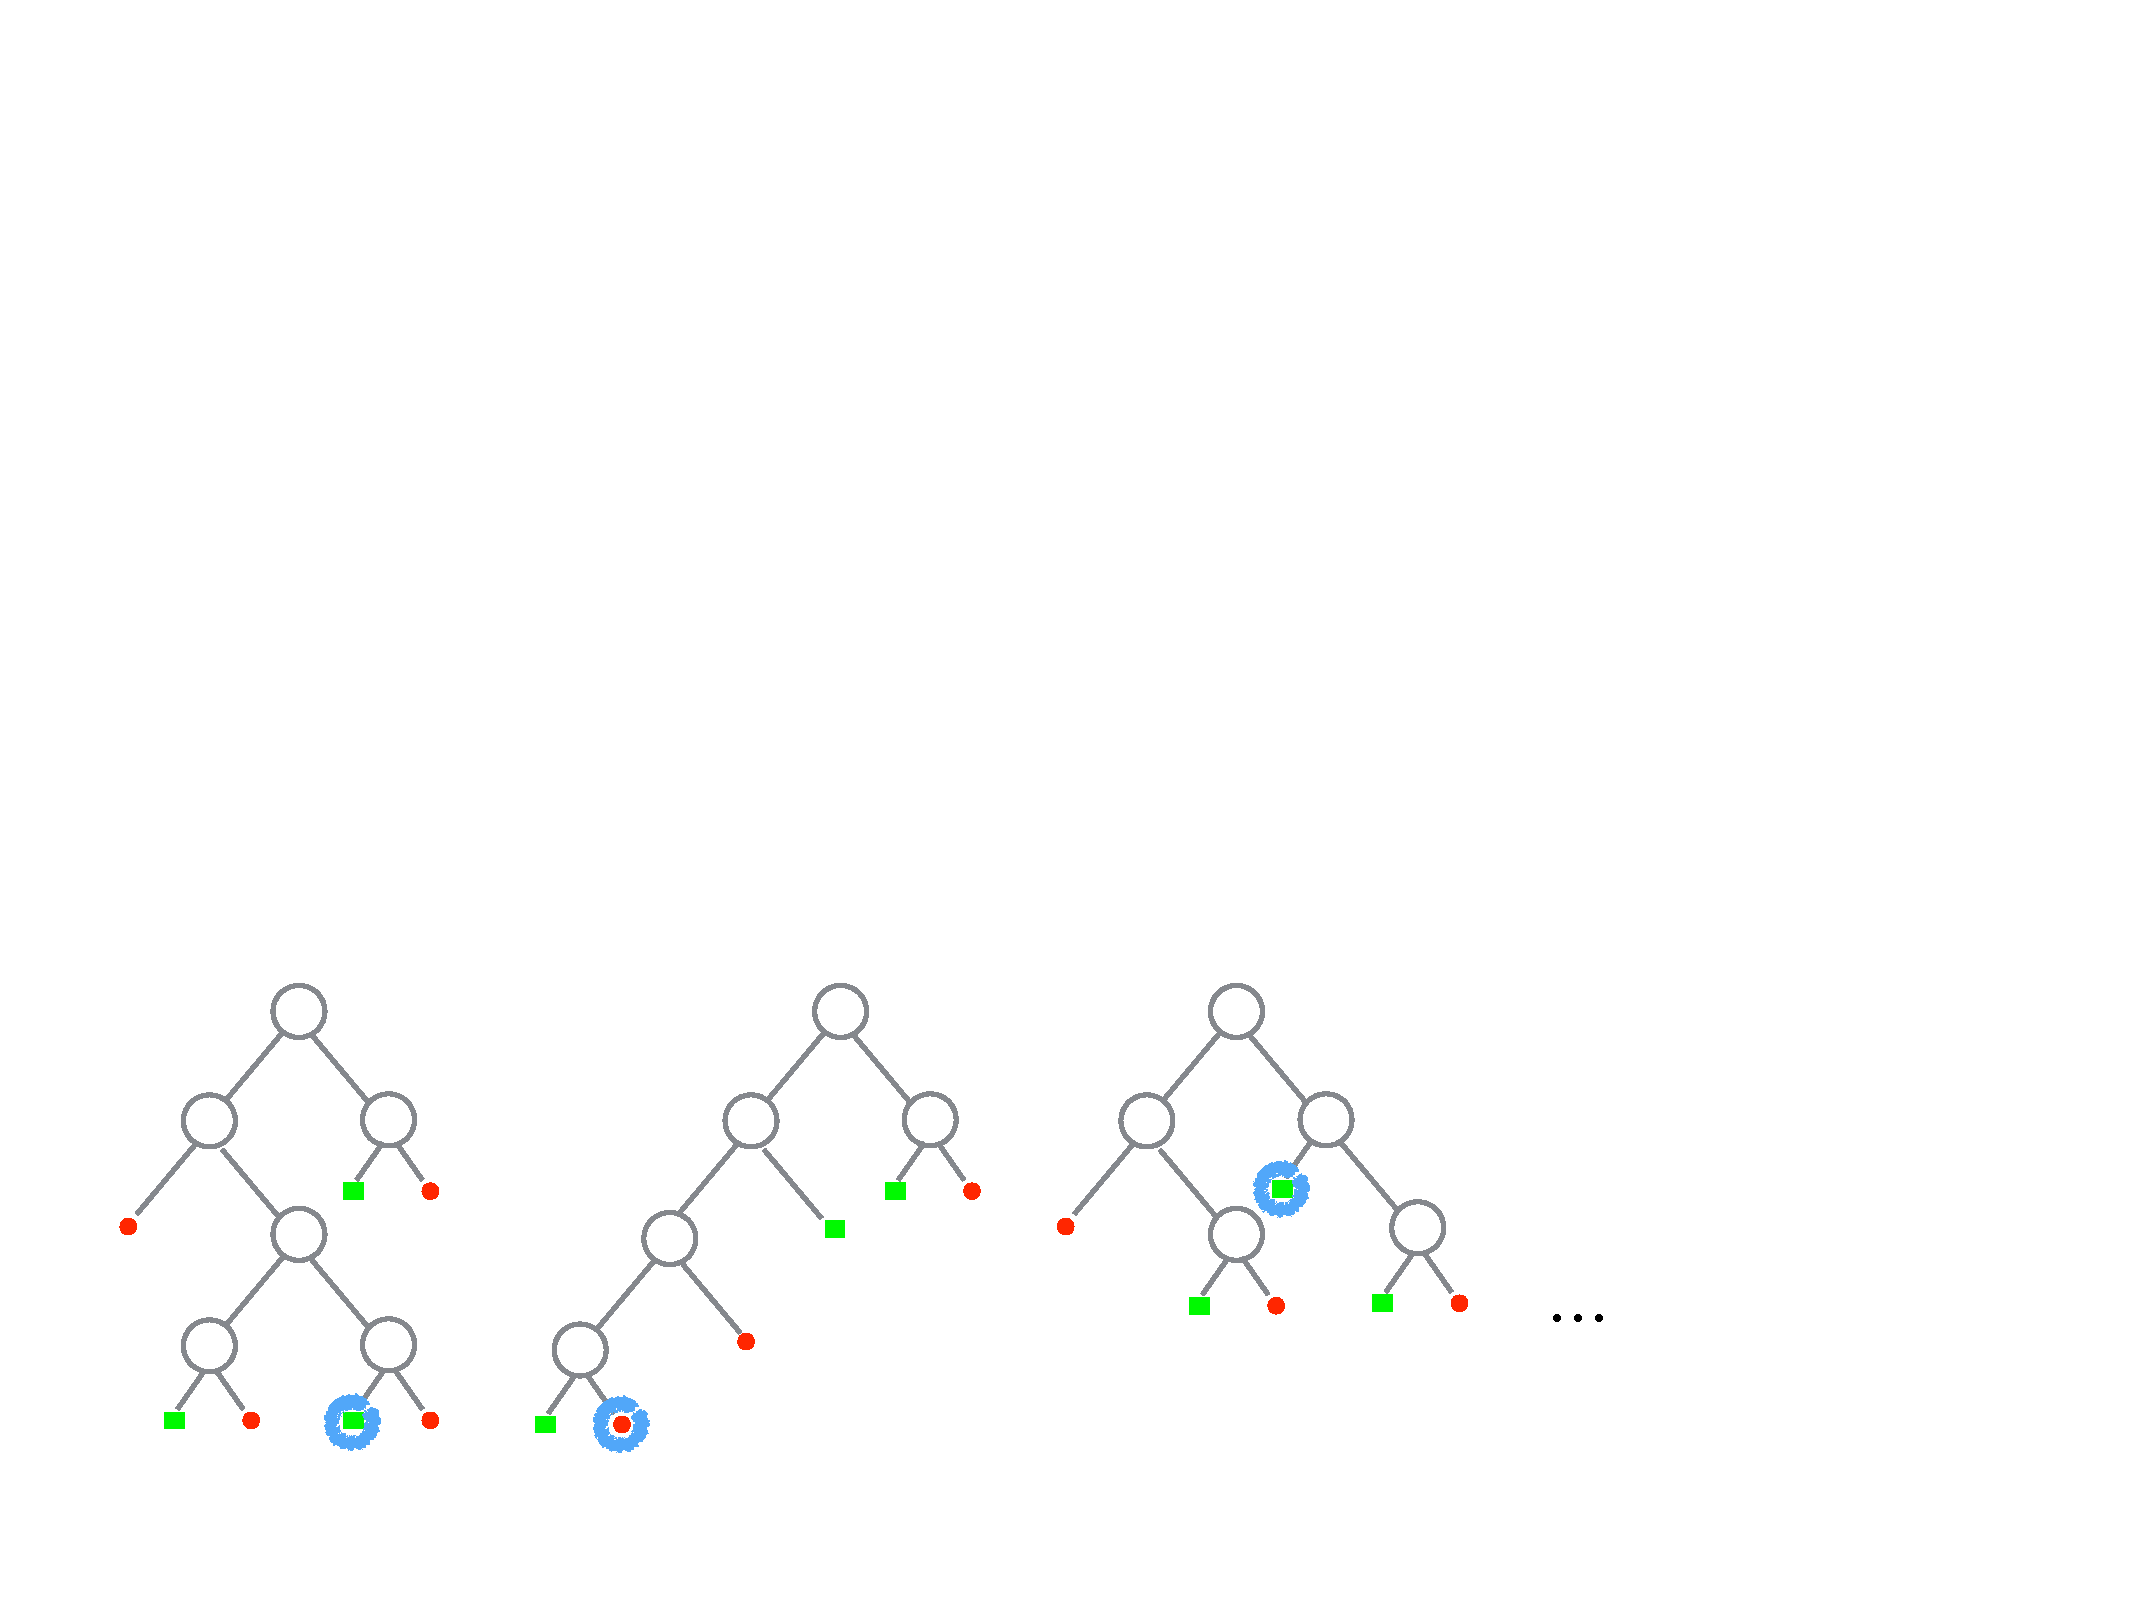
\includegraphics[width=0.8\textwidth]{../graphics/Forest.pdf}
% \end{figure}
% \begin{itemize}
% 	\item While decision trees can approximate very complicated decision boundaries, they tend to fit too much to the training data (overfitting).
% 	\item Random forests: set of decision trees, each learned on a different (randomly drawn) portion of the data and with different (randomly selected) features.
% 	\item Each tree gives a classification result.
% 	\item The final result is obtained by a majority vote.
% \end{itemize}
% \end{frame}


%\subsection{Nearest Neighbor classification}
\subsection{Random Forests}
\begin{frame}[plain,c]
\begin{center}
\Huge Random Forests
\end{center}
\end{frame}

% \begin{frame}{Random Forest: Decision trees}
% \begin{figure}[htb]
% 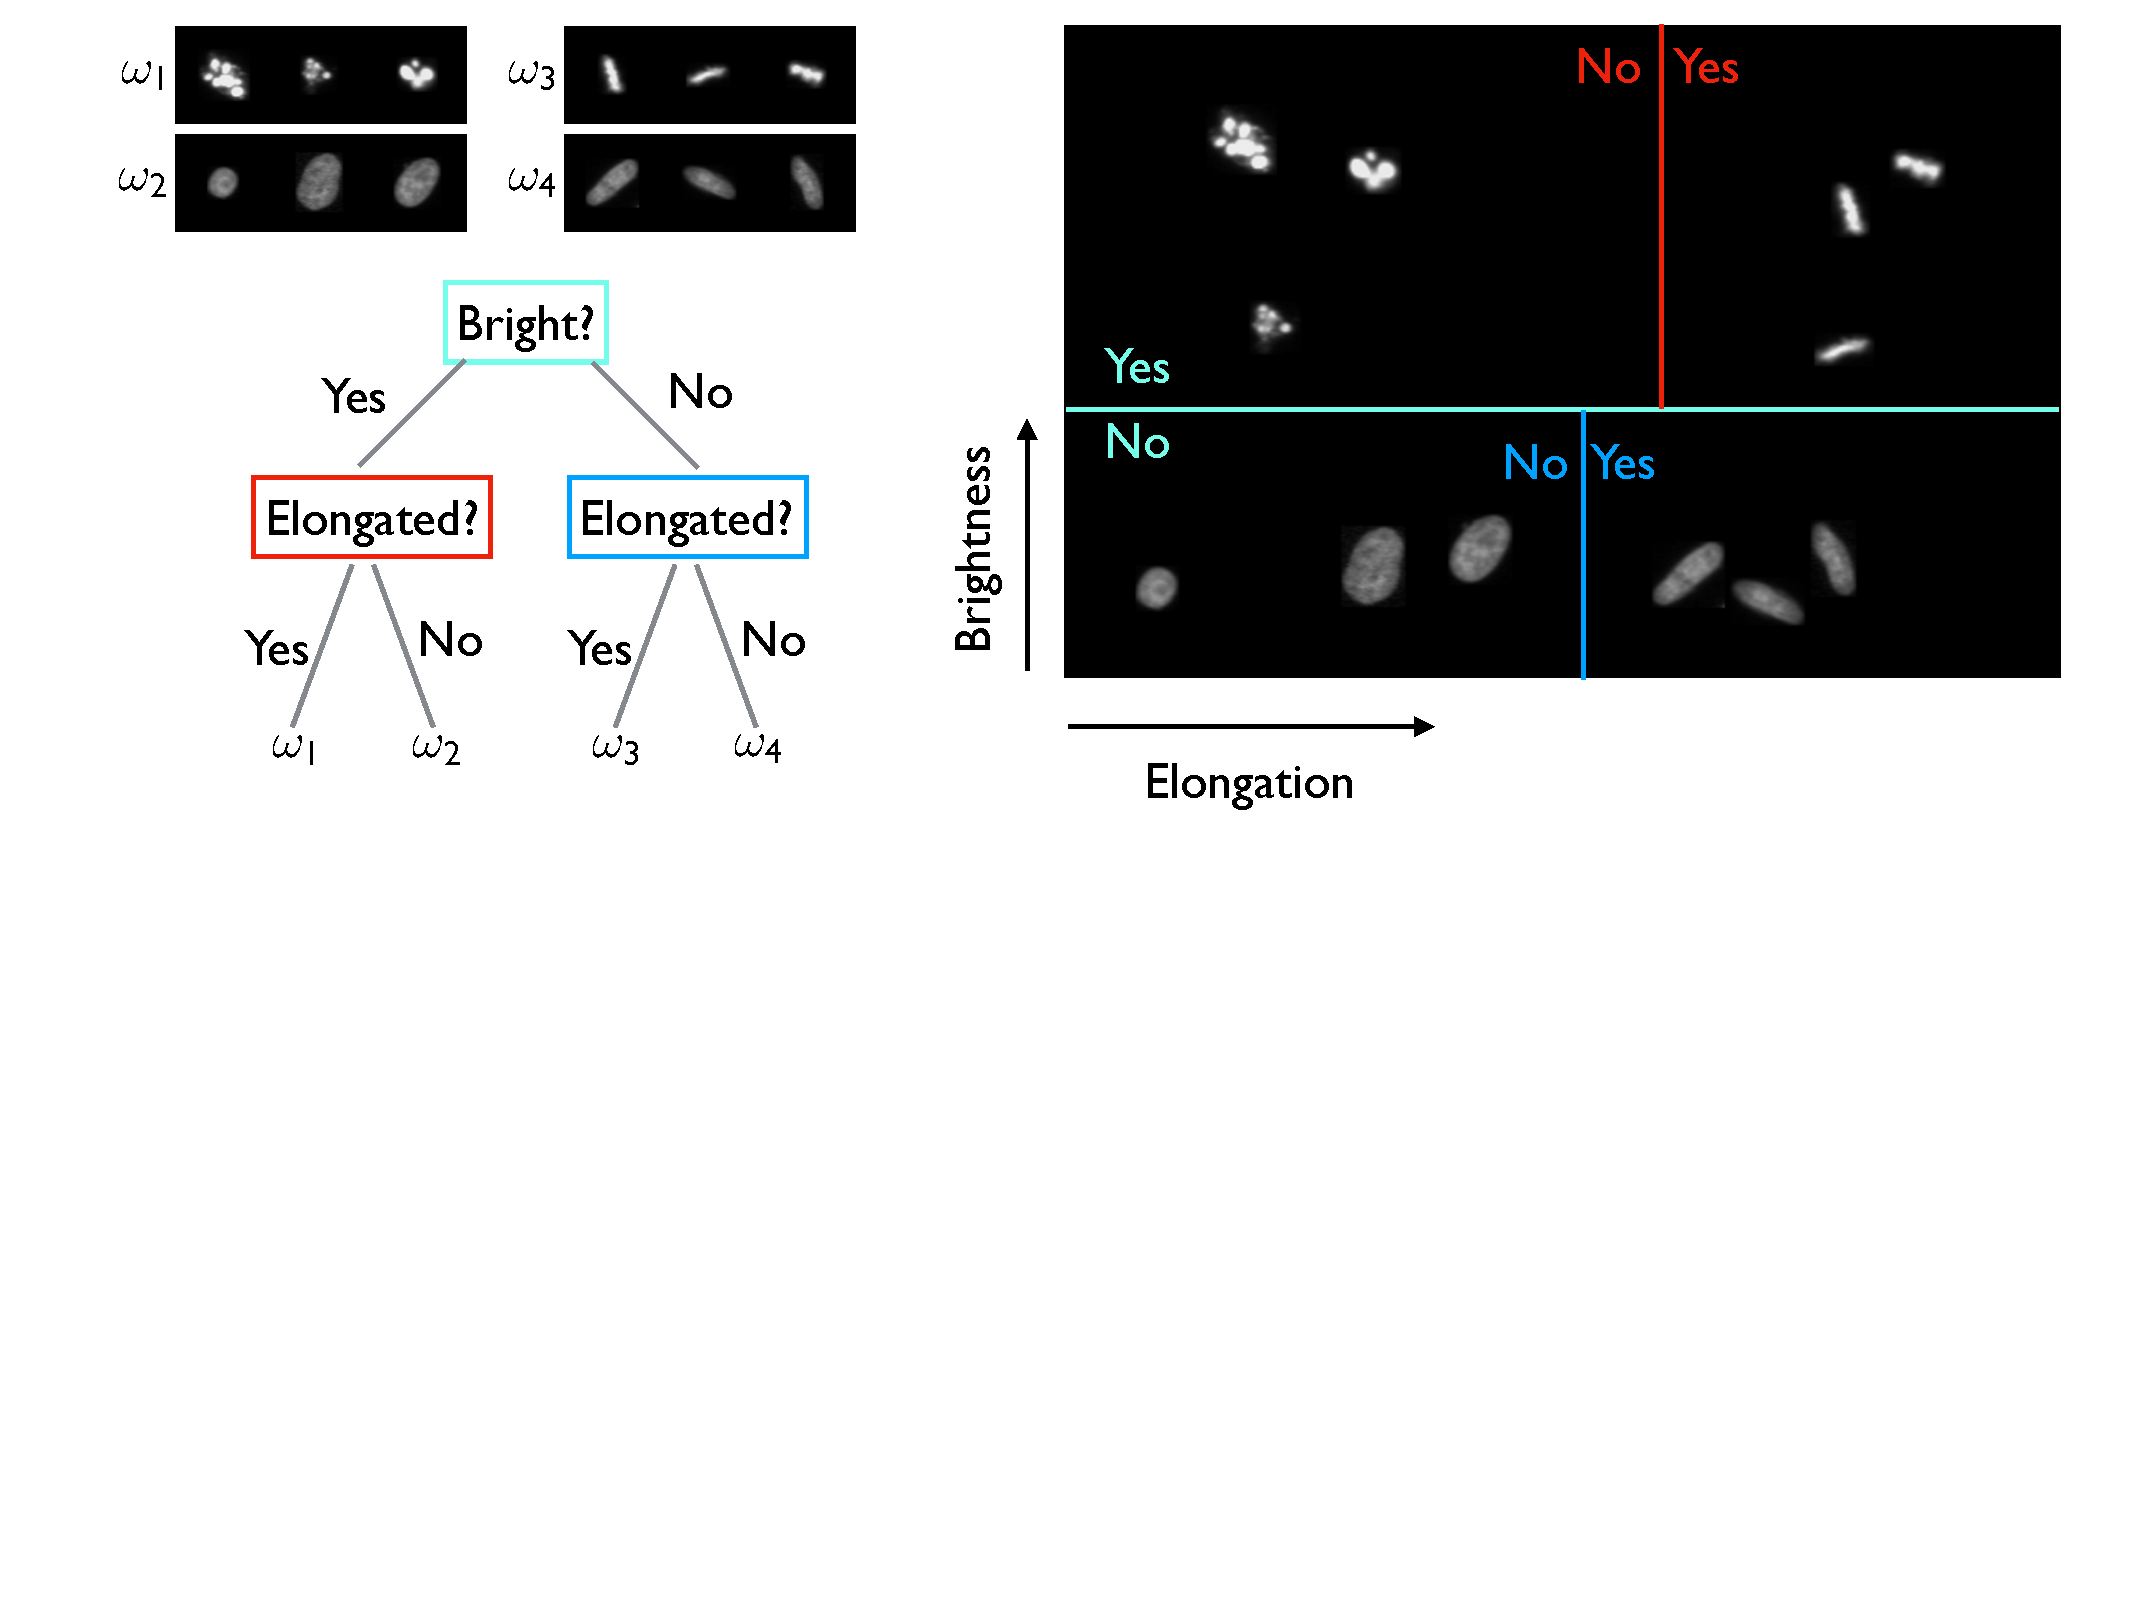
\includegraphics[width=0.8\textwidth]{../graphics/CellClassification_RF.pdf}
% \end{figure}

% \begin{itemize}
% 	\item Intuitive approach: applying a series of "rules" to the training data to recover the classes $\y_i$ (e.g. "is the cell bright?", "is the cell elongated?", ... )
% 	\item Each rule (or decision) divides the set of objects into two subsets.
% 	\item The whole classifier is thus represented by a decision tree, i.e. a hierarchically organized set of binary decisions.
% \end{itemize}
% \end{frame}

\begin{frame}{Random Forest: Decision trees}
\begin{figure}[htb]
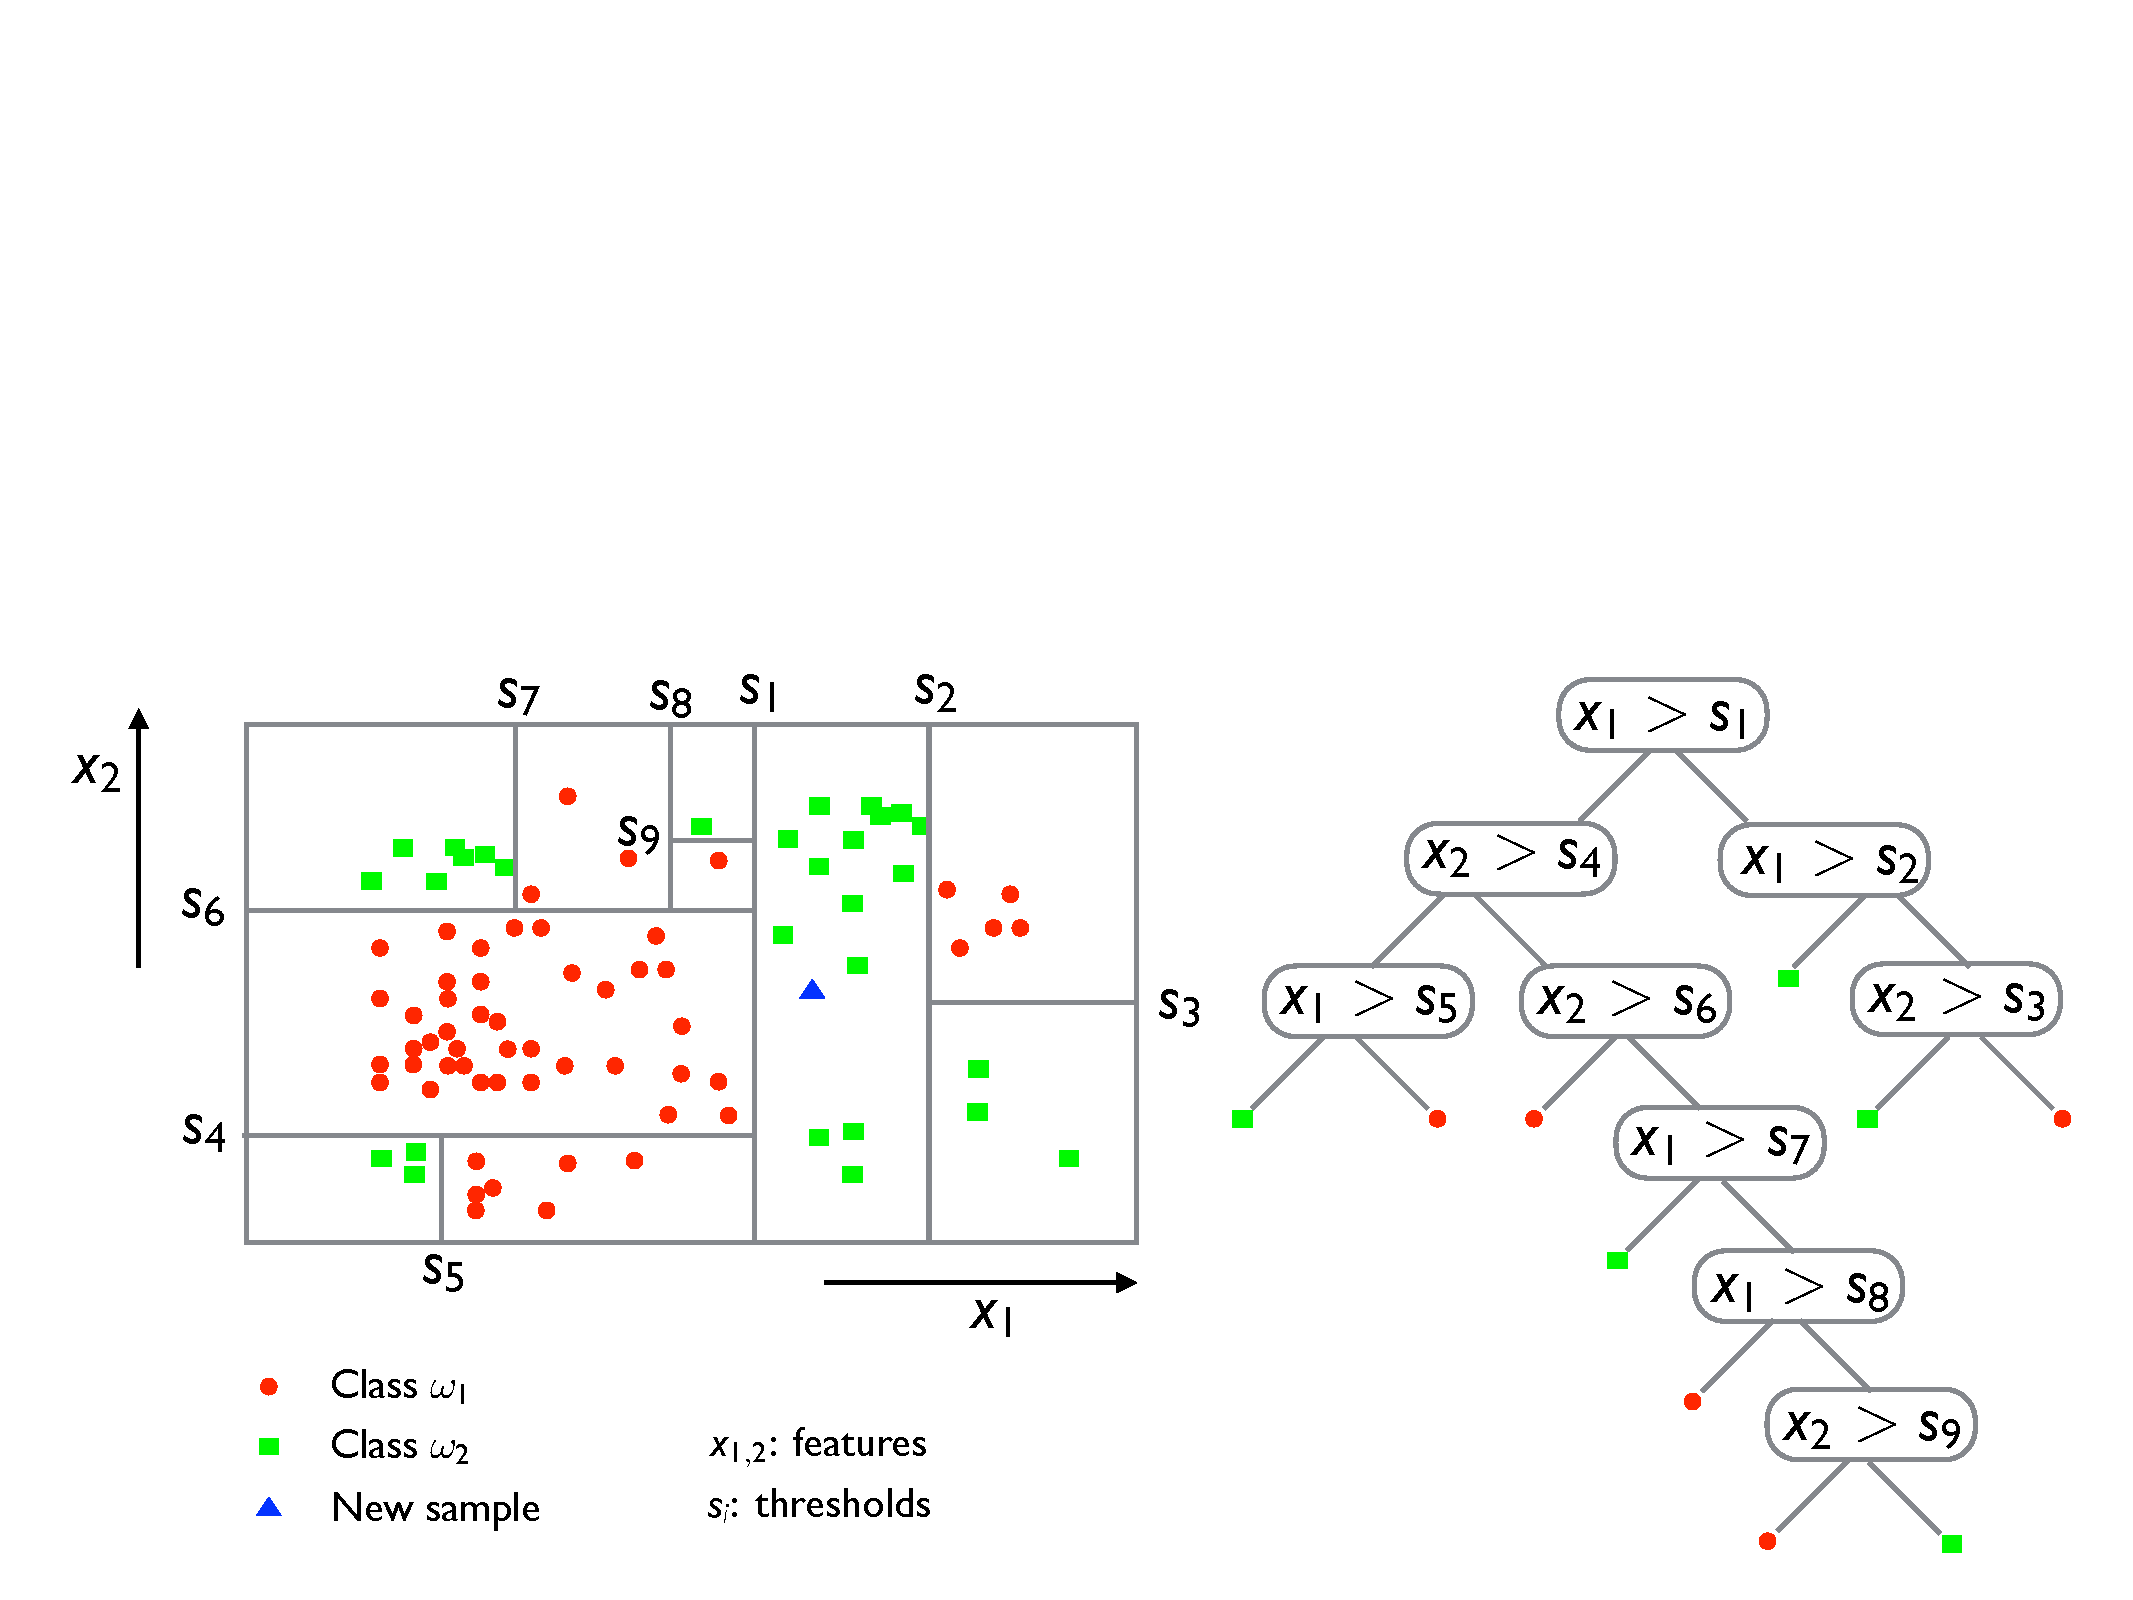
\includegraphics[width=0.8\textwidth]{../graphics/RF2.pdf}
\end{figure}
\begin{itemize}
	\item Decision trees correspond to a series of binary decisions that partition the feature space.
	\item Classification of a new object: application of the binary decision rules and assignment of the leaf label.
	\item The decision boundaries can be very complex and adapt very tightly to the training set.
\end{itemize}
\end{frame}

% \begin{frame}{Random Forest: Decision trees}
% \begin{itemize}
% \item Such decision trees can be built from data in an optimal way, by repeated division of the feature space.
% \item At every step, we split the data set into two, according to one feature.
% \item The feature and the threshold are chosen automatically in such a way that the resulting groups have best "purity".
% \item This can be achieved by minimizing the Gini impurity (GI) or entropy.
% % For $K$ classes, GINI impurity is defined as:
% % \begin{eqnarray*}
% % GI(R_m) &=& \sum_{k=1}^{K}\hat{p}_{mk}(1-\hat{p}_{mk}) \\
% % GI(s) &=& \sum_{R_m}=\frac{|R_m|}{N}GI(R_m)
% % \end{eqnarray*}
% % where $R_m$ are the sets resulting from the split $s$ and $\hat{p}_{mk}$ is the probability of a sample in $R_m$ to belong to class $k$.
% \end{itemize}
% \end{frame}

% \begin{frame}{Random Forest: GINI impurity}
% \begin{figure}[htb]
% 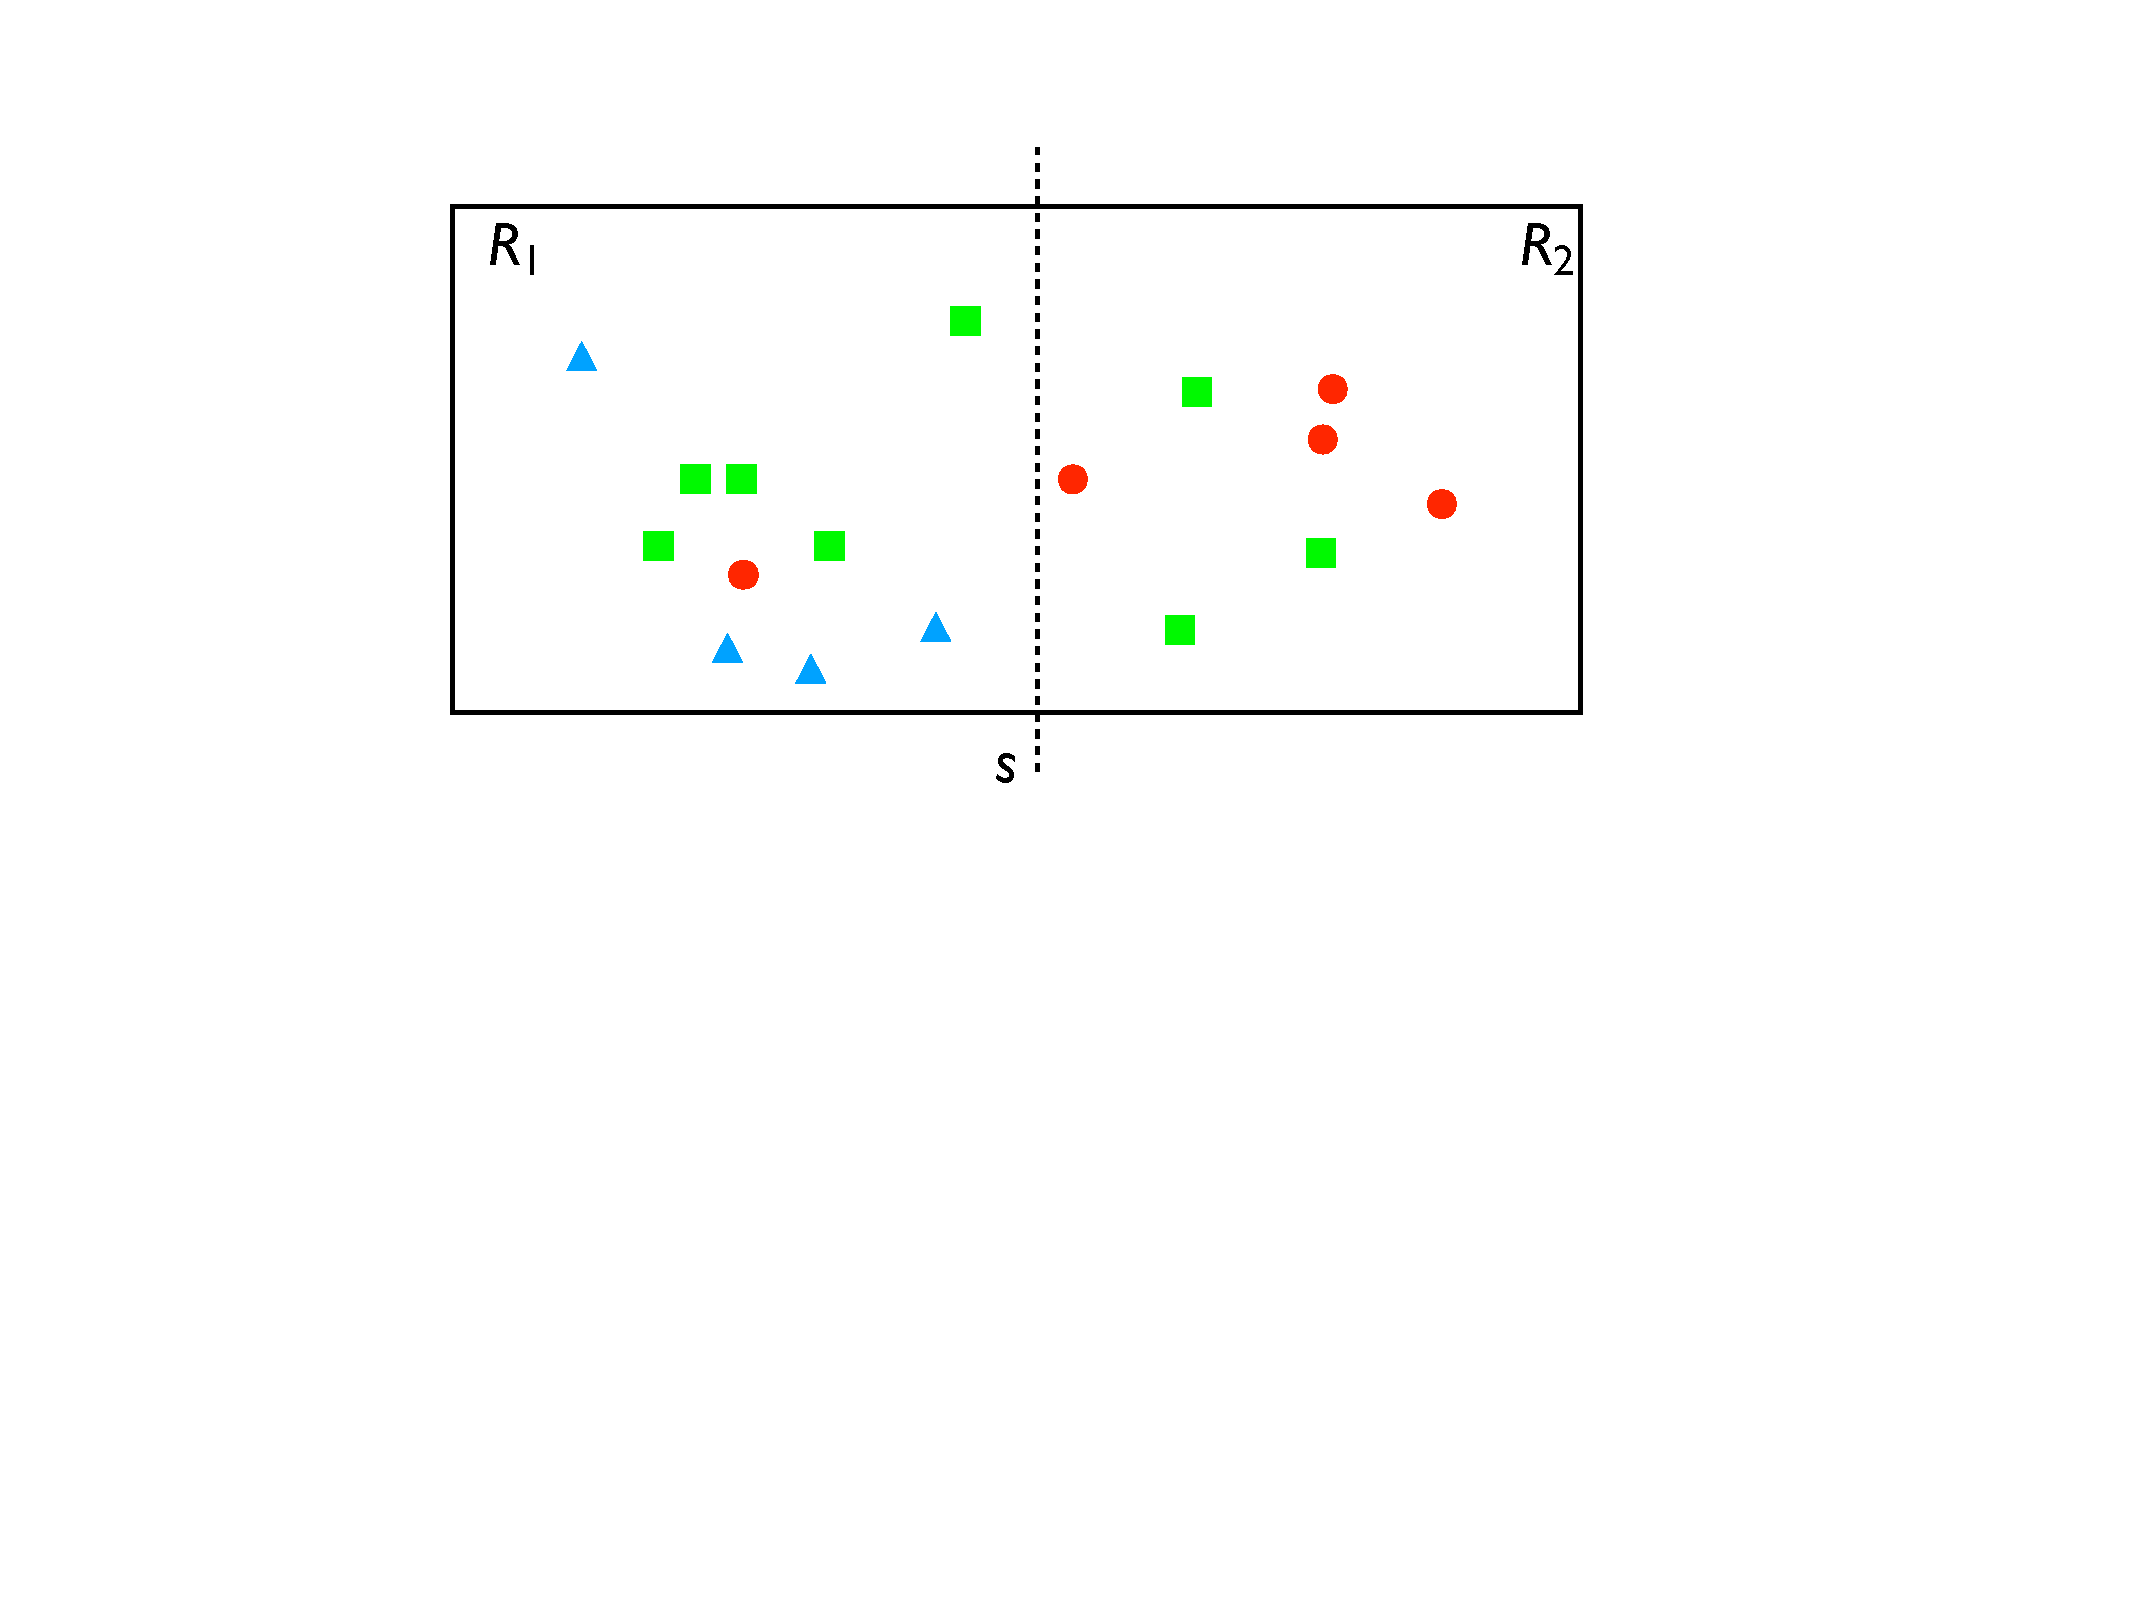
\includegraphics[width=0.7\textwidth]{../graphics/RF_GINI.pdf}
% \end{figure}
% Here, we obtain for the GINI impurity:
% \begin{eqnarray*}
% GI(R_1) &=&  \frac{1}{10} \cdot \frac{9}{10} + \frac{5}{10} \cdot \frac{5}{10} + \frac{4}{10} \cdot \frac{6}{10} = 0.58 \\
% GI(R_2) &=&  \frac{0}{7}\cdot \frac{7}{7} + \frac{4}{7} \cdot \frac{3}{7} + \frac{3}{7} \cdot \frac{4}{7} = 0.49 \\
% GI(s) &=&  \frac{10}{17}\cdot R_1 + \frac{7}{17}\cdot R_2 = 0.54
% \end{eqnarray*}
% \end{frame}

\begin{frame}{Random Forests}
\begin{figure}[htb]
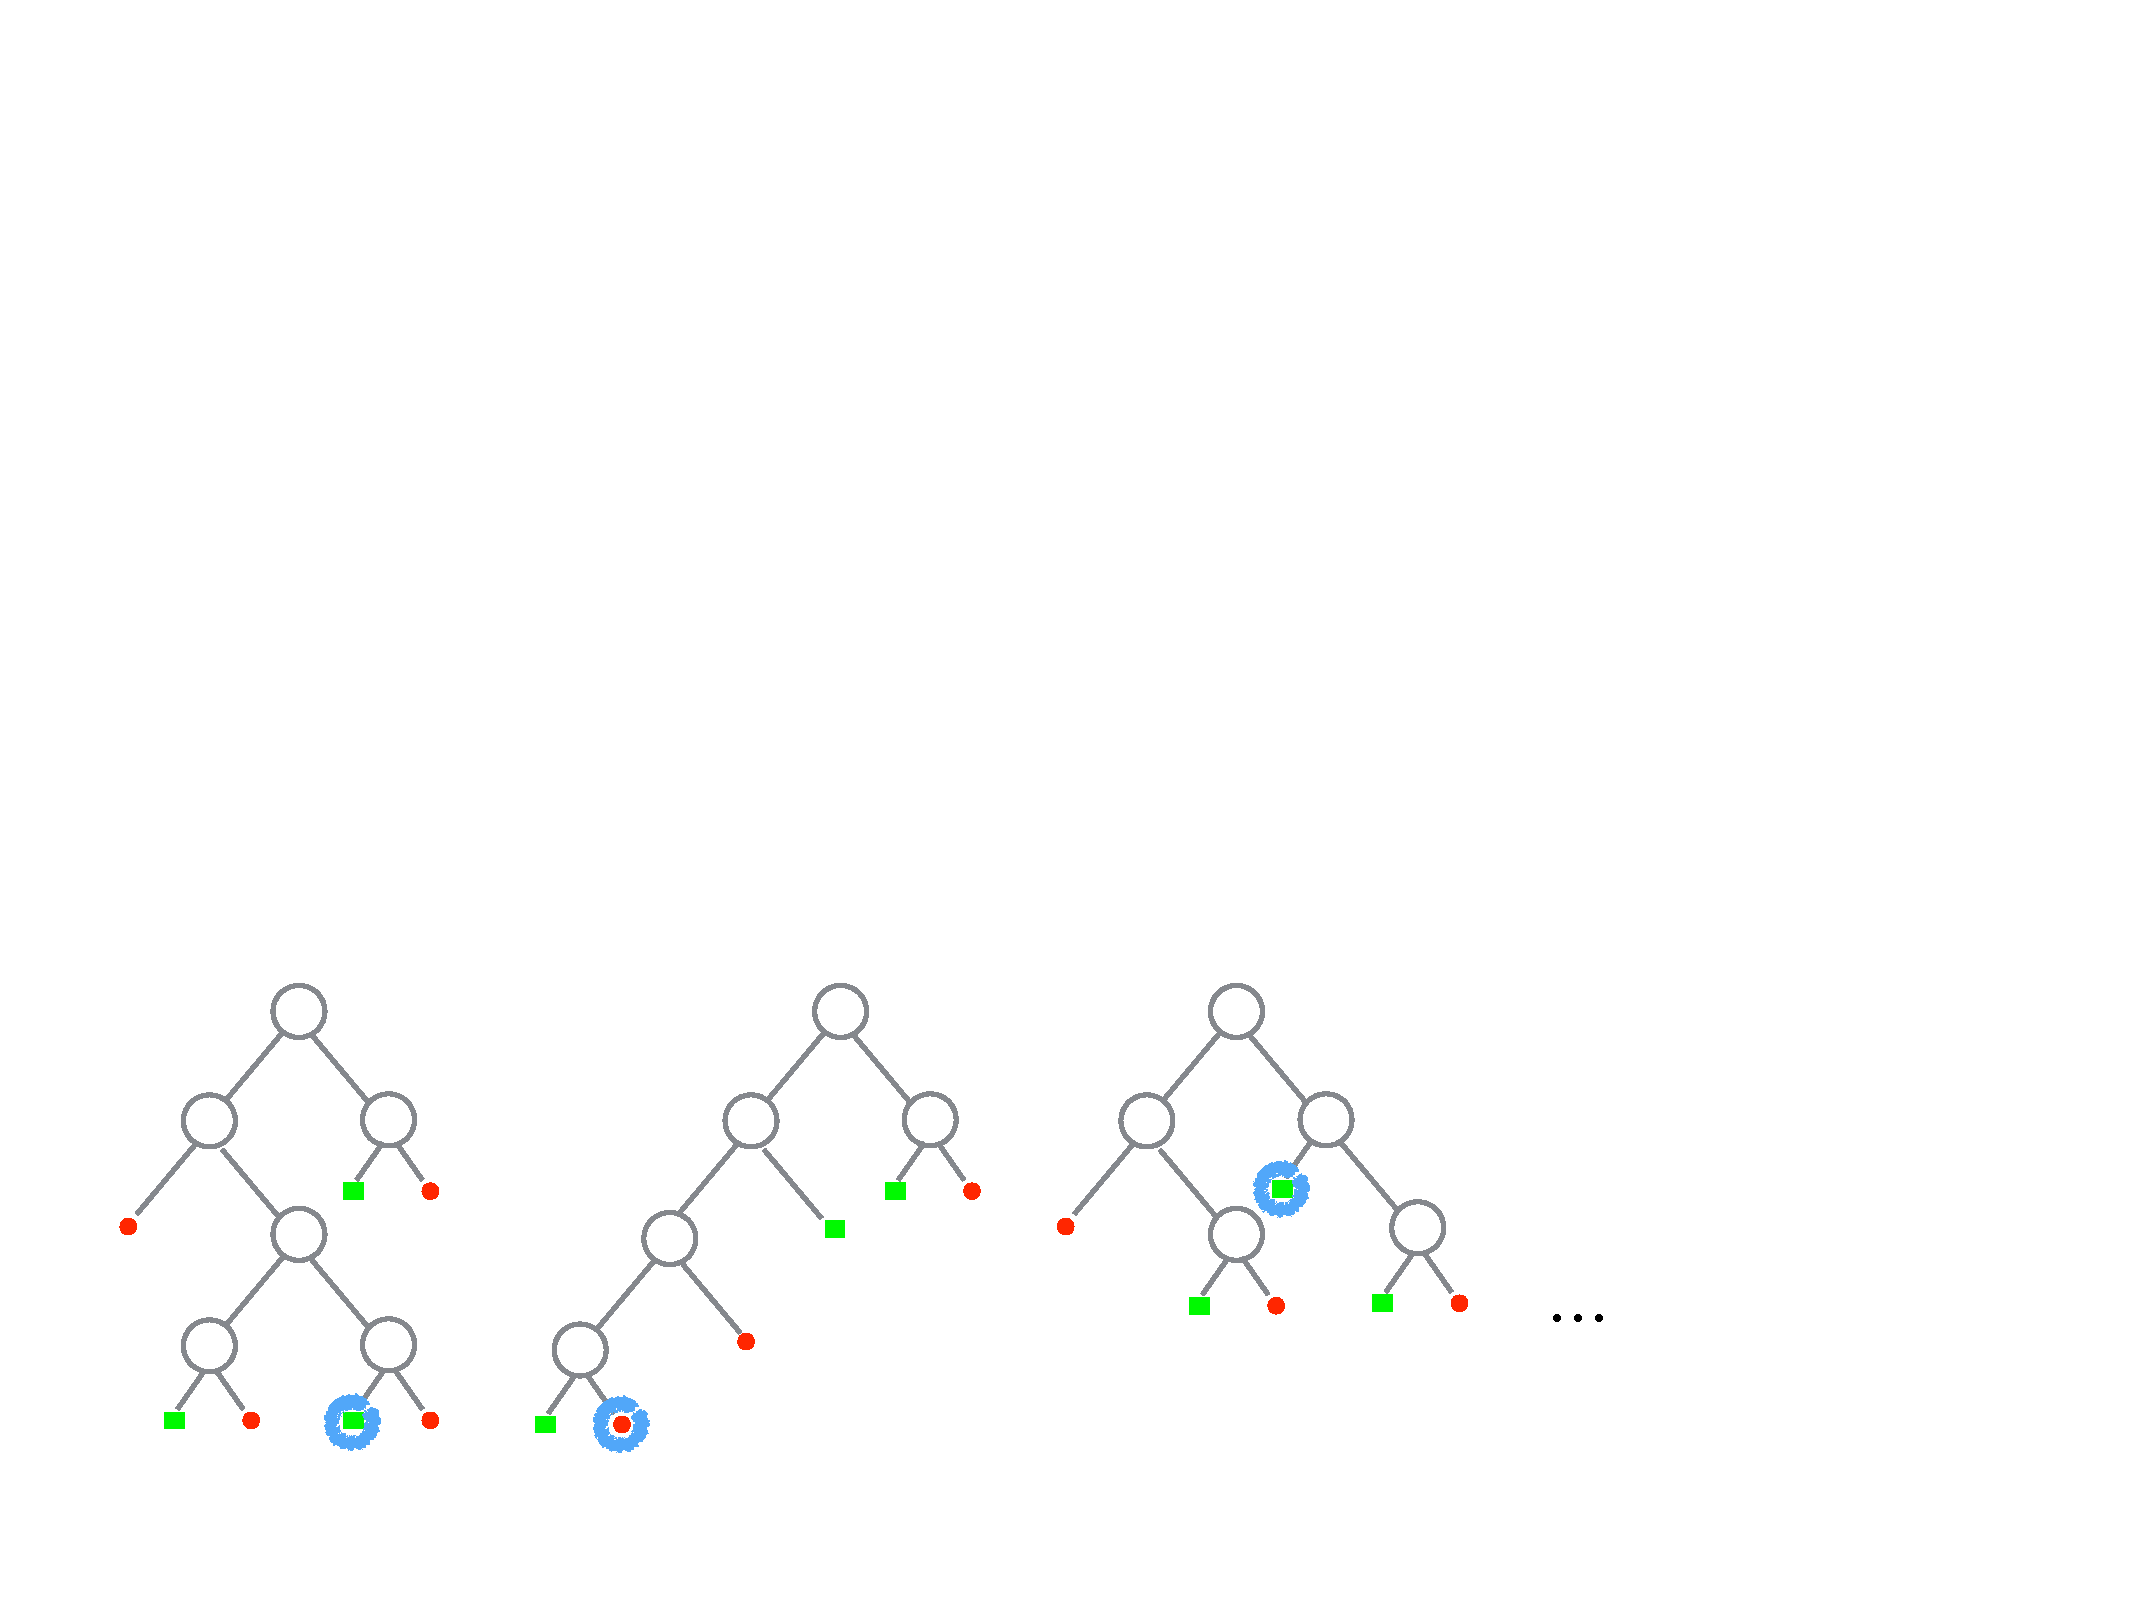
\includegraphics[width=0.8\textwidth]{../graphics/Forest.pdf}
\end{figure}
\begin{itemize}
	\item While decision trees can approximate very complicated decision boundaries, they tend to fit too much to the training data (overfitting).
	\item Random forests: set of decision trees, each learned on a different (randomly drawn) portion of the data and with different (randomly selected) features.
	\item Each tree gives a classification result.
	\item The final result is obtained by a majority vote.
\end{itemize}
\end{frame}

\begin{frame}{Random Forests}
\begin{itemize}
	\item Because each tree is slightly different from the others, each tree learns a slightly different aspect of the training data.
	\item A classification method that exists in averaging the results of several classifiers (often weak classifiers), is called {\bf ensemble method}.
	\item The strategy of averaging is a form of regularization.
	\item In practice, model averaging is very popular in the deep learning field. Often, one averages simply the output of several networks to obtain a more robust classifier.
\end{itemize}
\end{frame}

\subsection{Linear Discriminant Analysis (LDA)}
\begin{frame}[plain,c]
\begin{center}
\Huge Linear Discriminant Analysis
\end{center}
\end{frame}


% \begin{frame}{The Bayes rule of classification 1/4}
% \begin{block}{Product and sum rules of probabilities}
% 	Let $X$ and $Y$ be random variables, and let $P(X)$ and $P(Y)$ be their marginal probabilities, $P(X,Y)$ their joint probability and $P(X\,|\,Y)$ the conditional probability of $X$ given $Y$.
% 	\begin{itemize}
% 		\item Product rule:
% 		\begin{equation}
% 			P(X,Y) = P(X\,|\,Y)P(Y)
% 		\end{equation}
% 		\item Sum rule:
% 		\begin{equation}
% 			P(X) = \sum_Y P(X,Y) = \sum(P(X|Y)P(Y)
% 		\end{equation}
% 	\end{itemize}
% \end{block}
% Example: the probability that I am eaten be a shark in Australia is the probability to be in Australia times the probability to be eaten by a shark given that I am in Australia.
% \end{frame}

% \begin{frame}{The Bayes rule of classification 2/4}

% From the product rule and $P(X,Y)=P(Y,X)$ we get immediately the Bayes theorem:
% \begin{equation}
% 	P(Y \, | \, X) = \frac{P(X \, | \, Y)P(Y)}{P(X)}
% \end{equation}

% This rule holds for discrete variables, but almost identical rules hold in the case of continuous variables: we need to replace probabilities by probability densities (as the probability of observing one particular value of a continuous variable is often close to 0).

% % Here, we assume that $Y$ is a discrete variable (classes) and $X$ is a continuous variable (measurements). We thus obtain:
% % \begin{equation}
% % 	P(Y \, | \, X) = \frac{p(X \, | \, Y)P(Y)}{p(X)}
% % \end{equation}

% \end{frame}

\begin{frame}{The Bayes rule of classification 1/2}

\begin{block}{Bayes rule of classification}
	\textbf{Bayes Theorem}: Let $x \in \mathbb{R}^P$ with a probability density $p(x)$ and $y \in \{1 \ldots, K\}$ a discrete set of class labels. The posterior probability $P(y=k\,|\,x)$ can be written as:
	\begin{equation}
		P(y=k \, | \, x) = \frac{p(x \, | \, y=k) P(y=k)}{p(x)}
	\end{equation}
	\textbf{The Bayes rule of classification}: \emph{choose the class that maximizes the posterior probability} $P(y=k|x)$:
	\begin{equation}\label{equ:bayes_rule}
		\hat{y}(x) = \arg\max_k P(y=k \, | \, x) = \arg\max_k p(x\,|\,y=k)P(y=k)
	\end{equation}
\end{block}

\end{frame}


\begin{frame}{The Bayes rule of classification 2/2}
\begin{itemize}
\item The Bayes rule of classification simply states that the best class to choose is the one with highest probability given the observation.
\item Importantly, we can calculate this posterior probability from the class dependent feature distributions and the class probabilities.
\item This rule is important because it gives the best possible classifier, given that the class dependent feature distributions $p(x\,|\,y=k)$ and the class probabilities $P(y=k)$ are known.
\item However, this is normally not the case: these distributions need to be estimated from the training data.
\end{itemize}
\end{frame}

% \begin{frame}{The Bayes rule for classification in the binary case}

% For simplicity, we assume the case of binary classification, i.e. $y \in \{1, 2\}$. The Bayes rule for classification states that we should choose class $1$ if:

% \begin{equation*}
% \frac{p(x|y=1)P(y=1)}{p(x|y=2)P(y=2)} > 1
% \end{equation*}
% \\
% We can apply the $log$ to both sides of the equation. We obtain the following expression for the Bayes rule of classification:
% \begin{equation}\label{equ:lda:condition}
% \log{ \frac{p(x|y=1)P(y=1)}{p(x|y=2)P(y=2)} } > 0
% \end{equation}

% \end{frame}

\begin{frame}{Normality assumption}
\begin{figure}[htb]
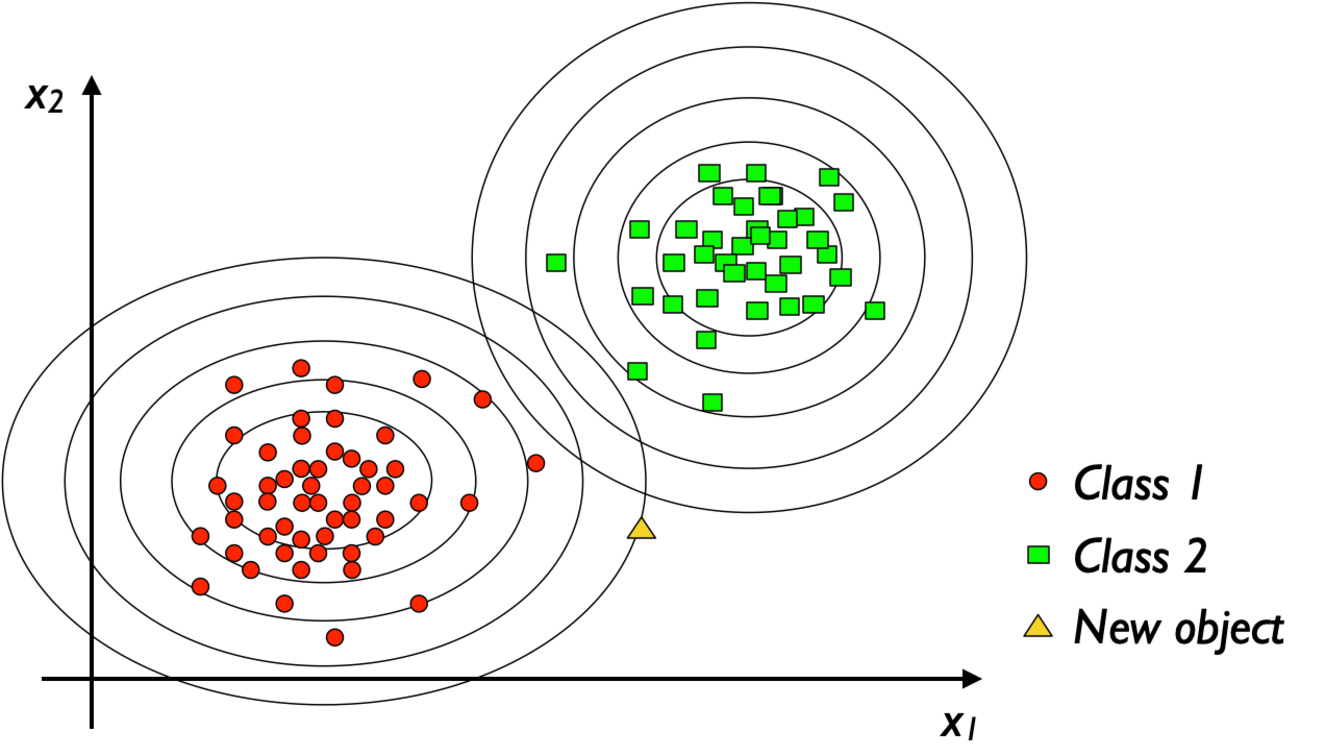
\includegraphics[width=0.8\textwidth]{../graphics/LDA3.pdf}
\end{figure}
We assume that features are normally distributed for each of the classes:
\begin{equation}\label{equ:lda:normal}
p(x|y=k)=\frac{1}{(2\pi)^{\frac{p}{2}}|\Sigma_k|^{\frac{1}{2}}}e^{-\frac{1}{2}(x-\mu_k)^T\Sigma_k^{-1}(x-\mu_k)}
\end{equation}
\end{frame}

\begin{frame}{Linear Discriminant Analysis (LDA)}
Plugging equation (\ref{equ:lda:normal}) into (\ref{equ:bayes_rule}) and the additional assumption that the covariance matrices of the classes are equal, i.e. $\Sigma_1 = \Sigma_2 = \Sigma$, we obtain {\bf Linear Discriminant Analysis, LDA}:
\begin{equation*}
\log{\frac{P(y=1)}{P(y=2)}} + x^T\Sigma^{-1}(\mu_1-\mu_2) - \frac{1}{2}(\mu_1-\mu_2)^T\Sigma^{-1}(\mu_1+\mu_2) > 0
\end{equation*}
\begin{itemize}
	\item We see that this is a linear classifier: $x$ is multiplied with $\Sigma^{-1}(\mu_1-\mu_2)$.
	\item $LDA$ is an old technique, but it is still used in practice.
	\item With neural networks, we typically aim at predicting posterior probabilities without parametric modeling of class dependent densities.
\end{itemize}
\end{frame}

% \begin{frame}{Comparison LDA vs. closest mean 1/2}
% \begin{itemize}
% 	\item Closest Mean Classifier:
% 	\begin{itemize}
% 		\item Calculate the mean value for each of the classes (from the training set).
% 		\item Rule: for a new vector $x \in \mathbb{R}^P$ assign the class with the closest mean, i.e. choose class $\omega_1$ if :
% 		\begin{eqnarray*}
% 		\|x - \mu_1\| &<& \|x - \mu_2\| \\
% 		(x-\mu_1)^T(x-\mu_1) - (x-\mu_2)^T(x-\mu_2) &<& 0 \\
% 		x^T(\mu_2 - \mu_1) + \frac{1}{2}(\|\mu_1\|^2 - \|\mu_2\|^2) &<& 0 \\
% 		x^T(\mu_1 - \mu_2) + b &>& 0
% 		\end{eqnarray*}
% 	\end{itemize}
% 	\item We see that the only term that depends on $x$ is linear and corresponds to a projection of $x$ onto the difference vector of the two class means $\mu_1$ and $\mu_2$.
% \end{itemize}
% \end{frame}

% \begin{frame}{Comparison LDA vs. closest mean 2/2}
% 	\begin{figure}[htb]
% 		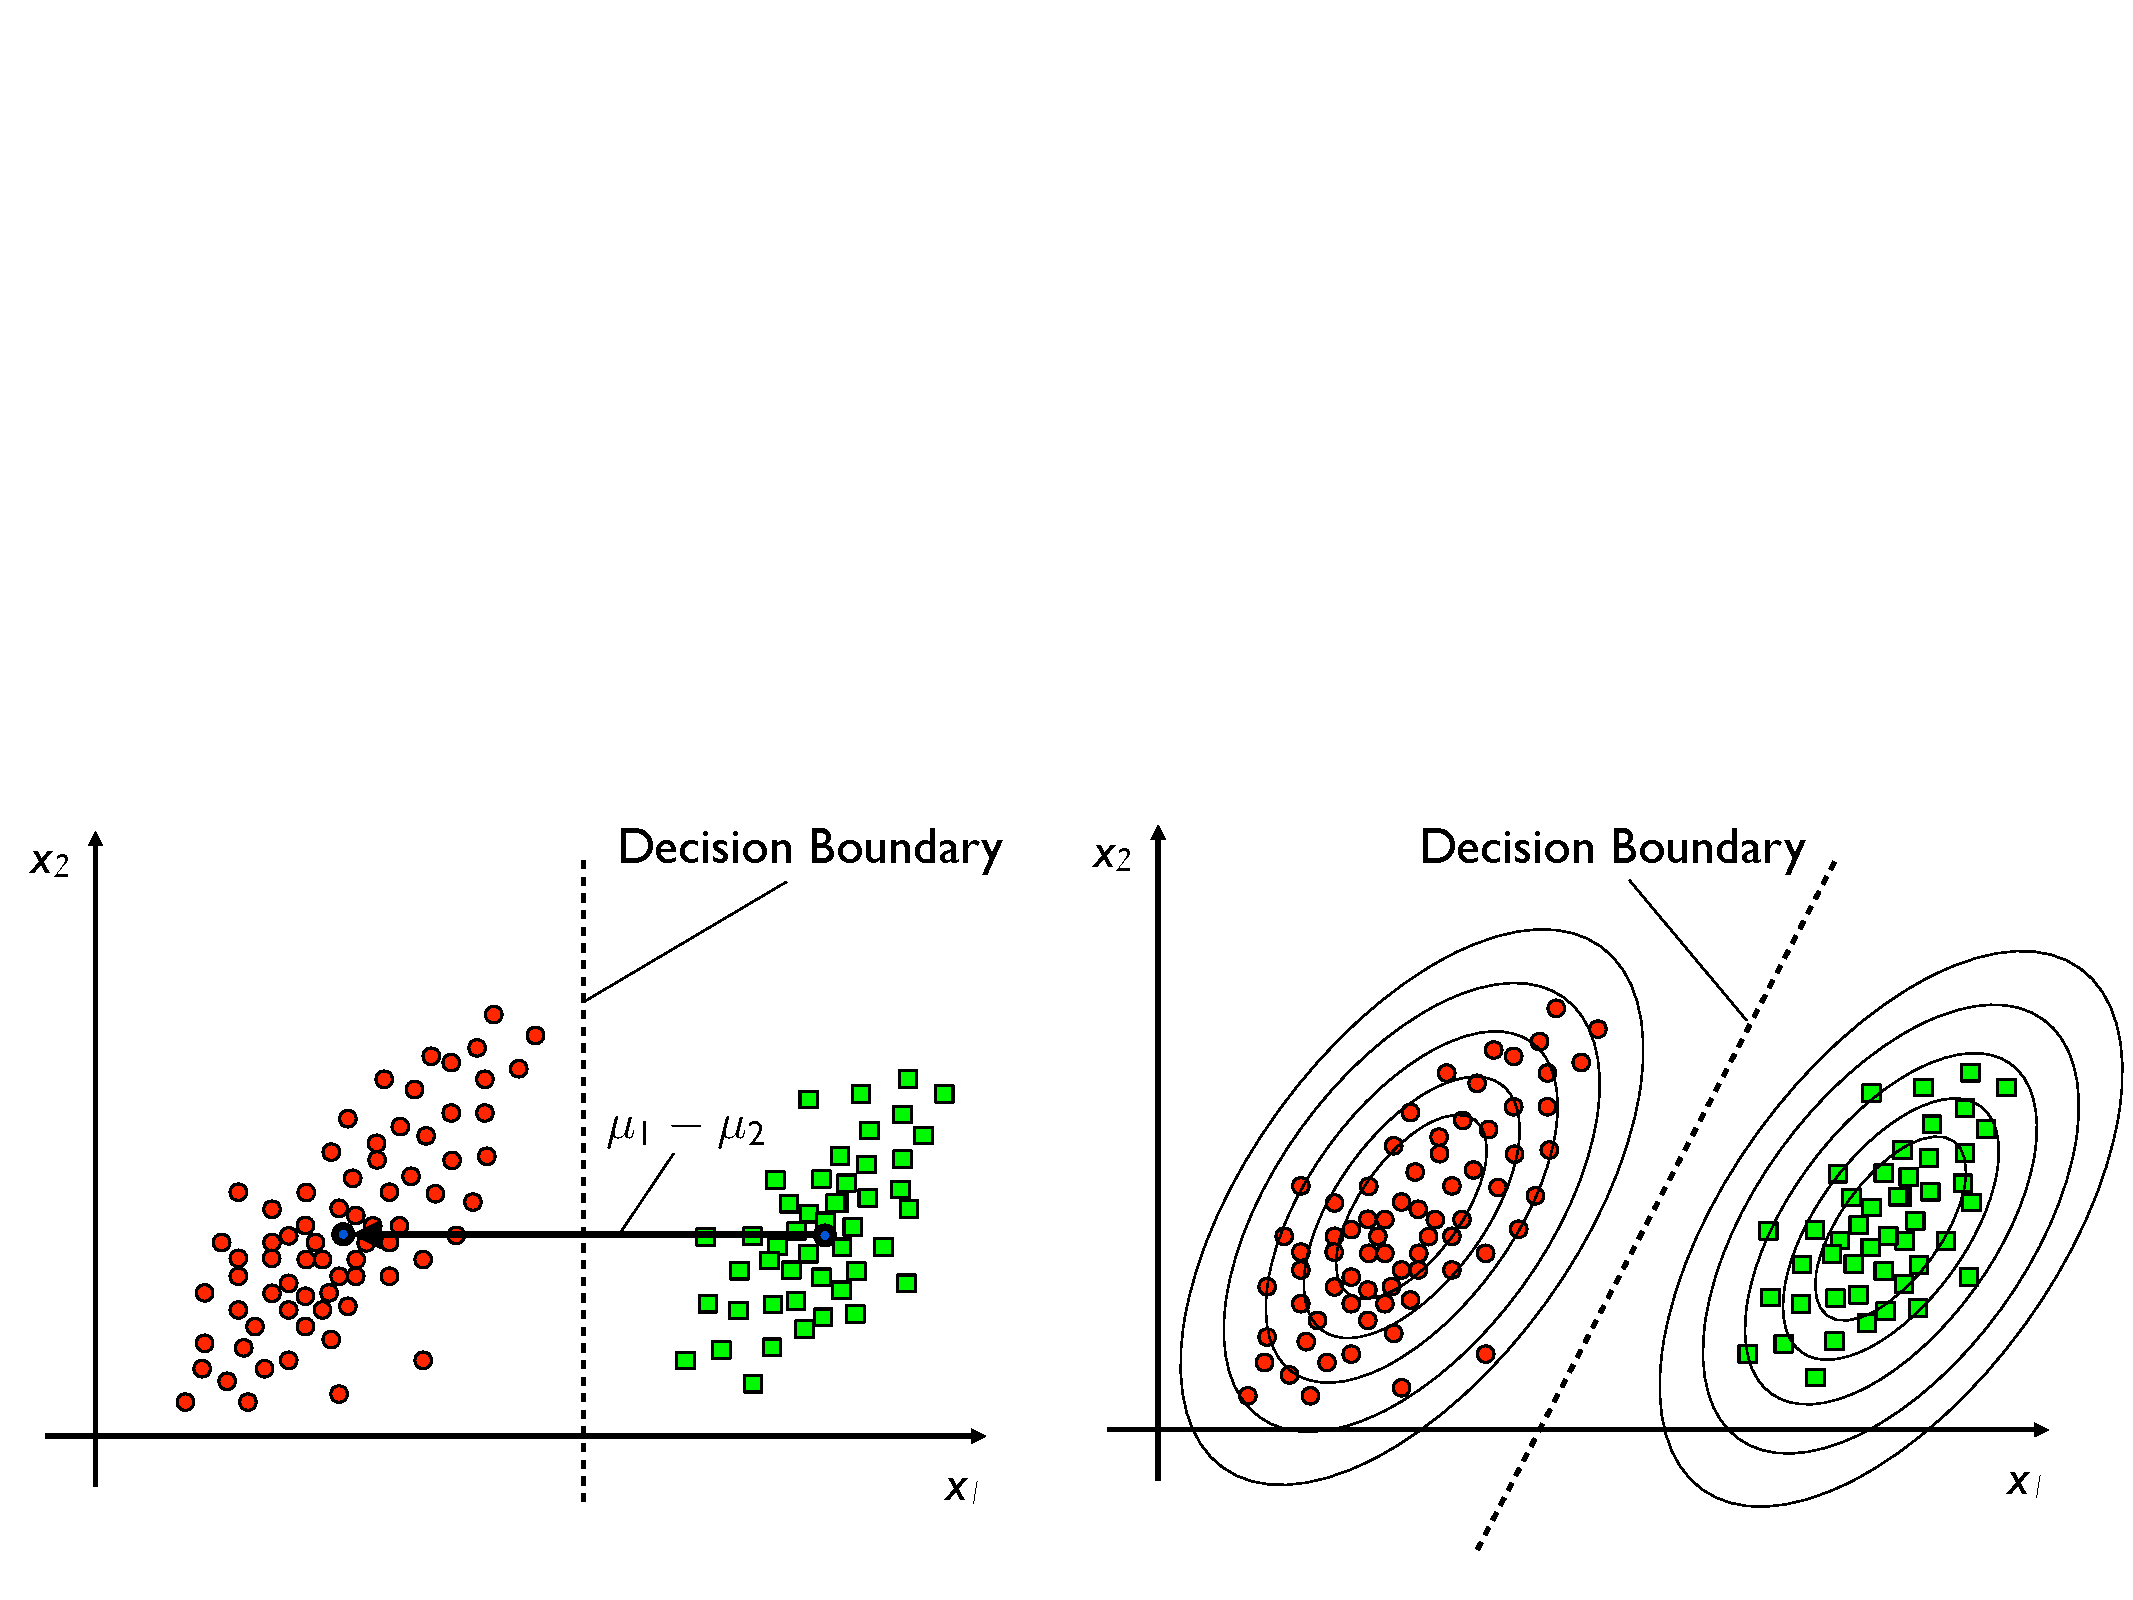
\includegraphics[width=0.8\textwidth]{../graphics/LDA_projection.pdf}
% 	\end{figure}
% 	\begin{itemize}
% 		\item The expression for LDA classification is:
% 		\begin{equation*}
% 			x^T\Sigma^{-1}(\mu_1-\mu_2) + b > 0
% 		\end{equation*}
% 		\item We thus see that the only difference is that we take the covariance matrix $\Sigma$ into account.
% 		\item The normal vector of the separating hyperplane is thus not $(\mu_1-\mu_2)$ but $\Sigma^{-1}(\mu_1-\mu_2)$.
% 	\end{itemize}
% \end{frame}

\subsection{Support Vector Machines (SVM) and kernel methods}
\begin{frame}[plain,c]
\begin{center}
\Huge Support Vector Machines
\end{center}
\end{frame}

\begin{frame}{Support Vector Machines: principle}
	\begin{figure}[htb]
		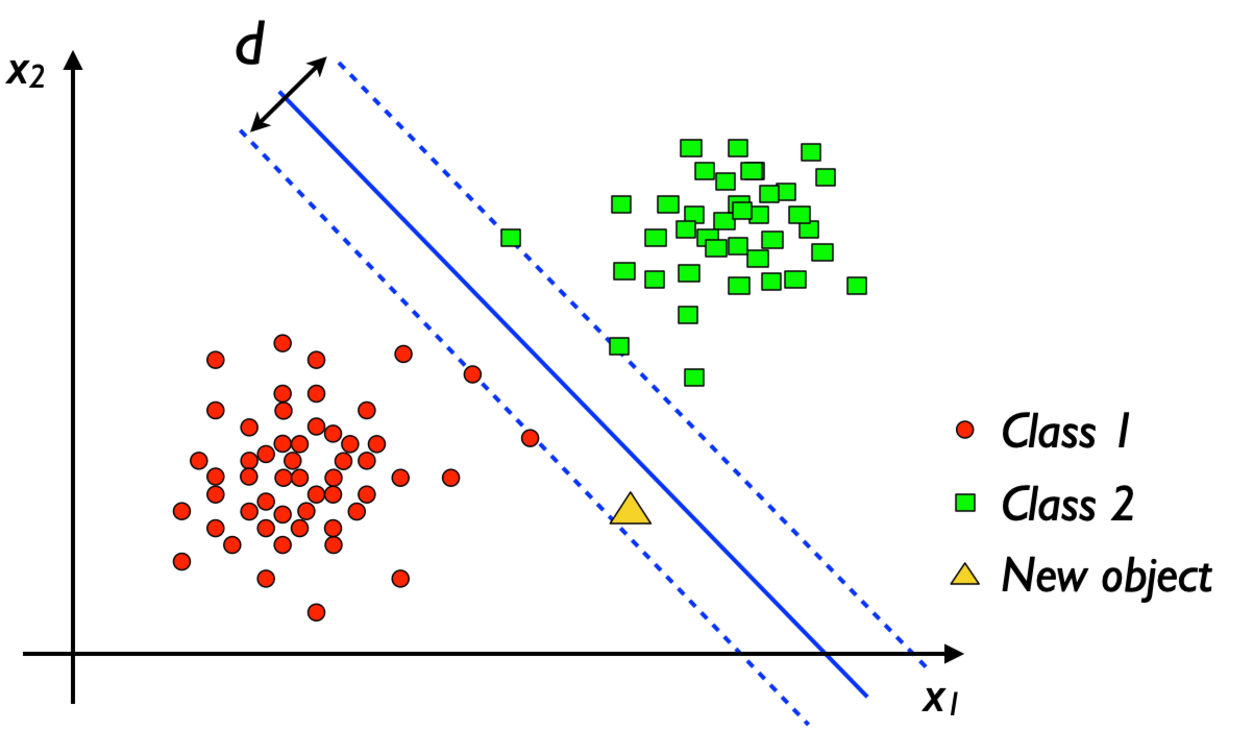
\includegraphics[width=0.8\textwidth]{../graphics/SVM_general.pdf}
	\end{figure}
	\begin{itemize}
		\item Optimal placement of a linear decision boundary.
		\item Intuitive approach: place a "ribbon" instead of a single line, i.e. two parallel lines separated by a distance $d$.
		\item Maximization of the width $d$ in order to push the separating hyperplane away from the two classes.
	\end{itemize}
\end{frame}

% \begin{frame}{Support Vector Machines: a convex optimization problem}
% 	\begin{figure}[htb]
% 		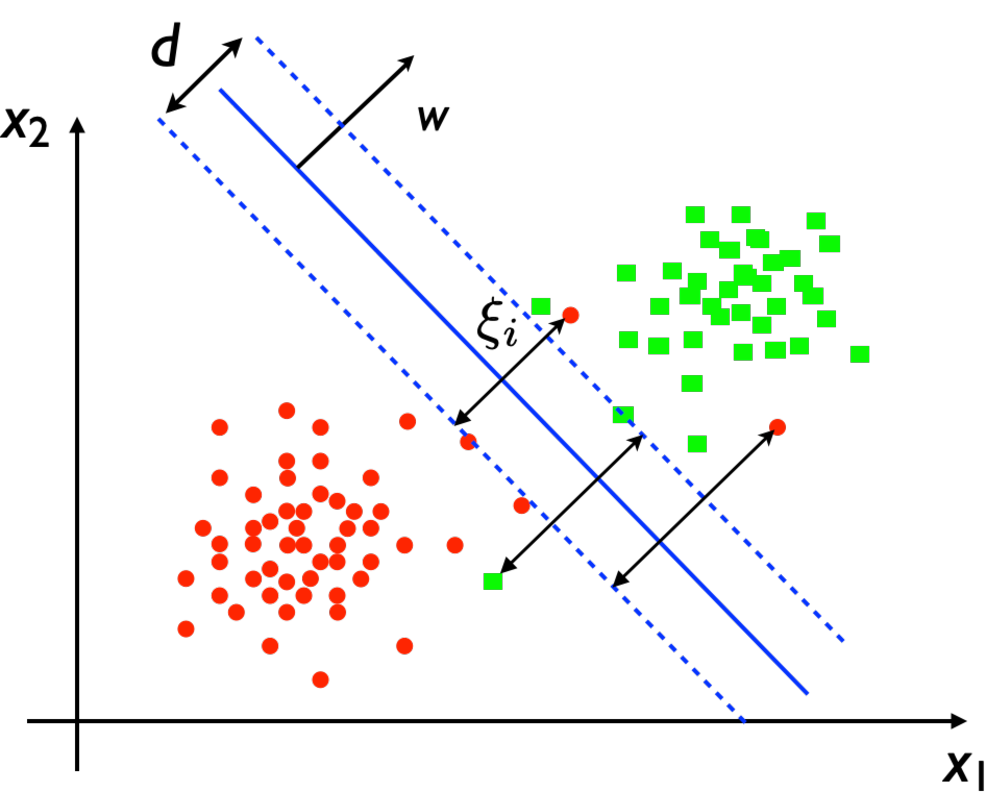
\includegraphics[width=0.5\textwidth]{../graphics/SVM_nonsep.pdf}
% 	\end{figure}
% 	\begin{itemize}
% 		\item Maximizing the width corresponds to minimizing the norm of the normal vector of the hyperplane $\|w\| = \frac{2}{d}$.
% 		\item In the case of linearly non-separable data, we need to find a compromise between error term $\sum_{i=1}^{N}\xi_i$ and regularization $\|w\|^2$ (we omit the constraints here):
% 		\begin{equation*}
% 			\min_{w,\xi} \|w\|^2 + C \sum_{i=1}^{N}\xi_i
% 		\end{equation*}
% 		\item We note that this corresponds to the general formulation we have seen before.
% 	\end{itemize}
% \end{frame}

% \begin{frame}{Support Vector Machines: linearly separable training set}
% 	\begin{figure}[htb]
% 		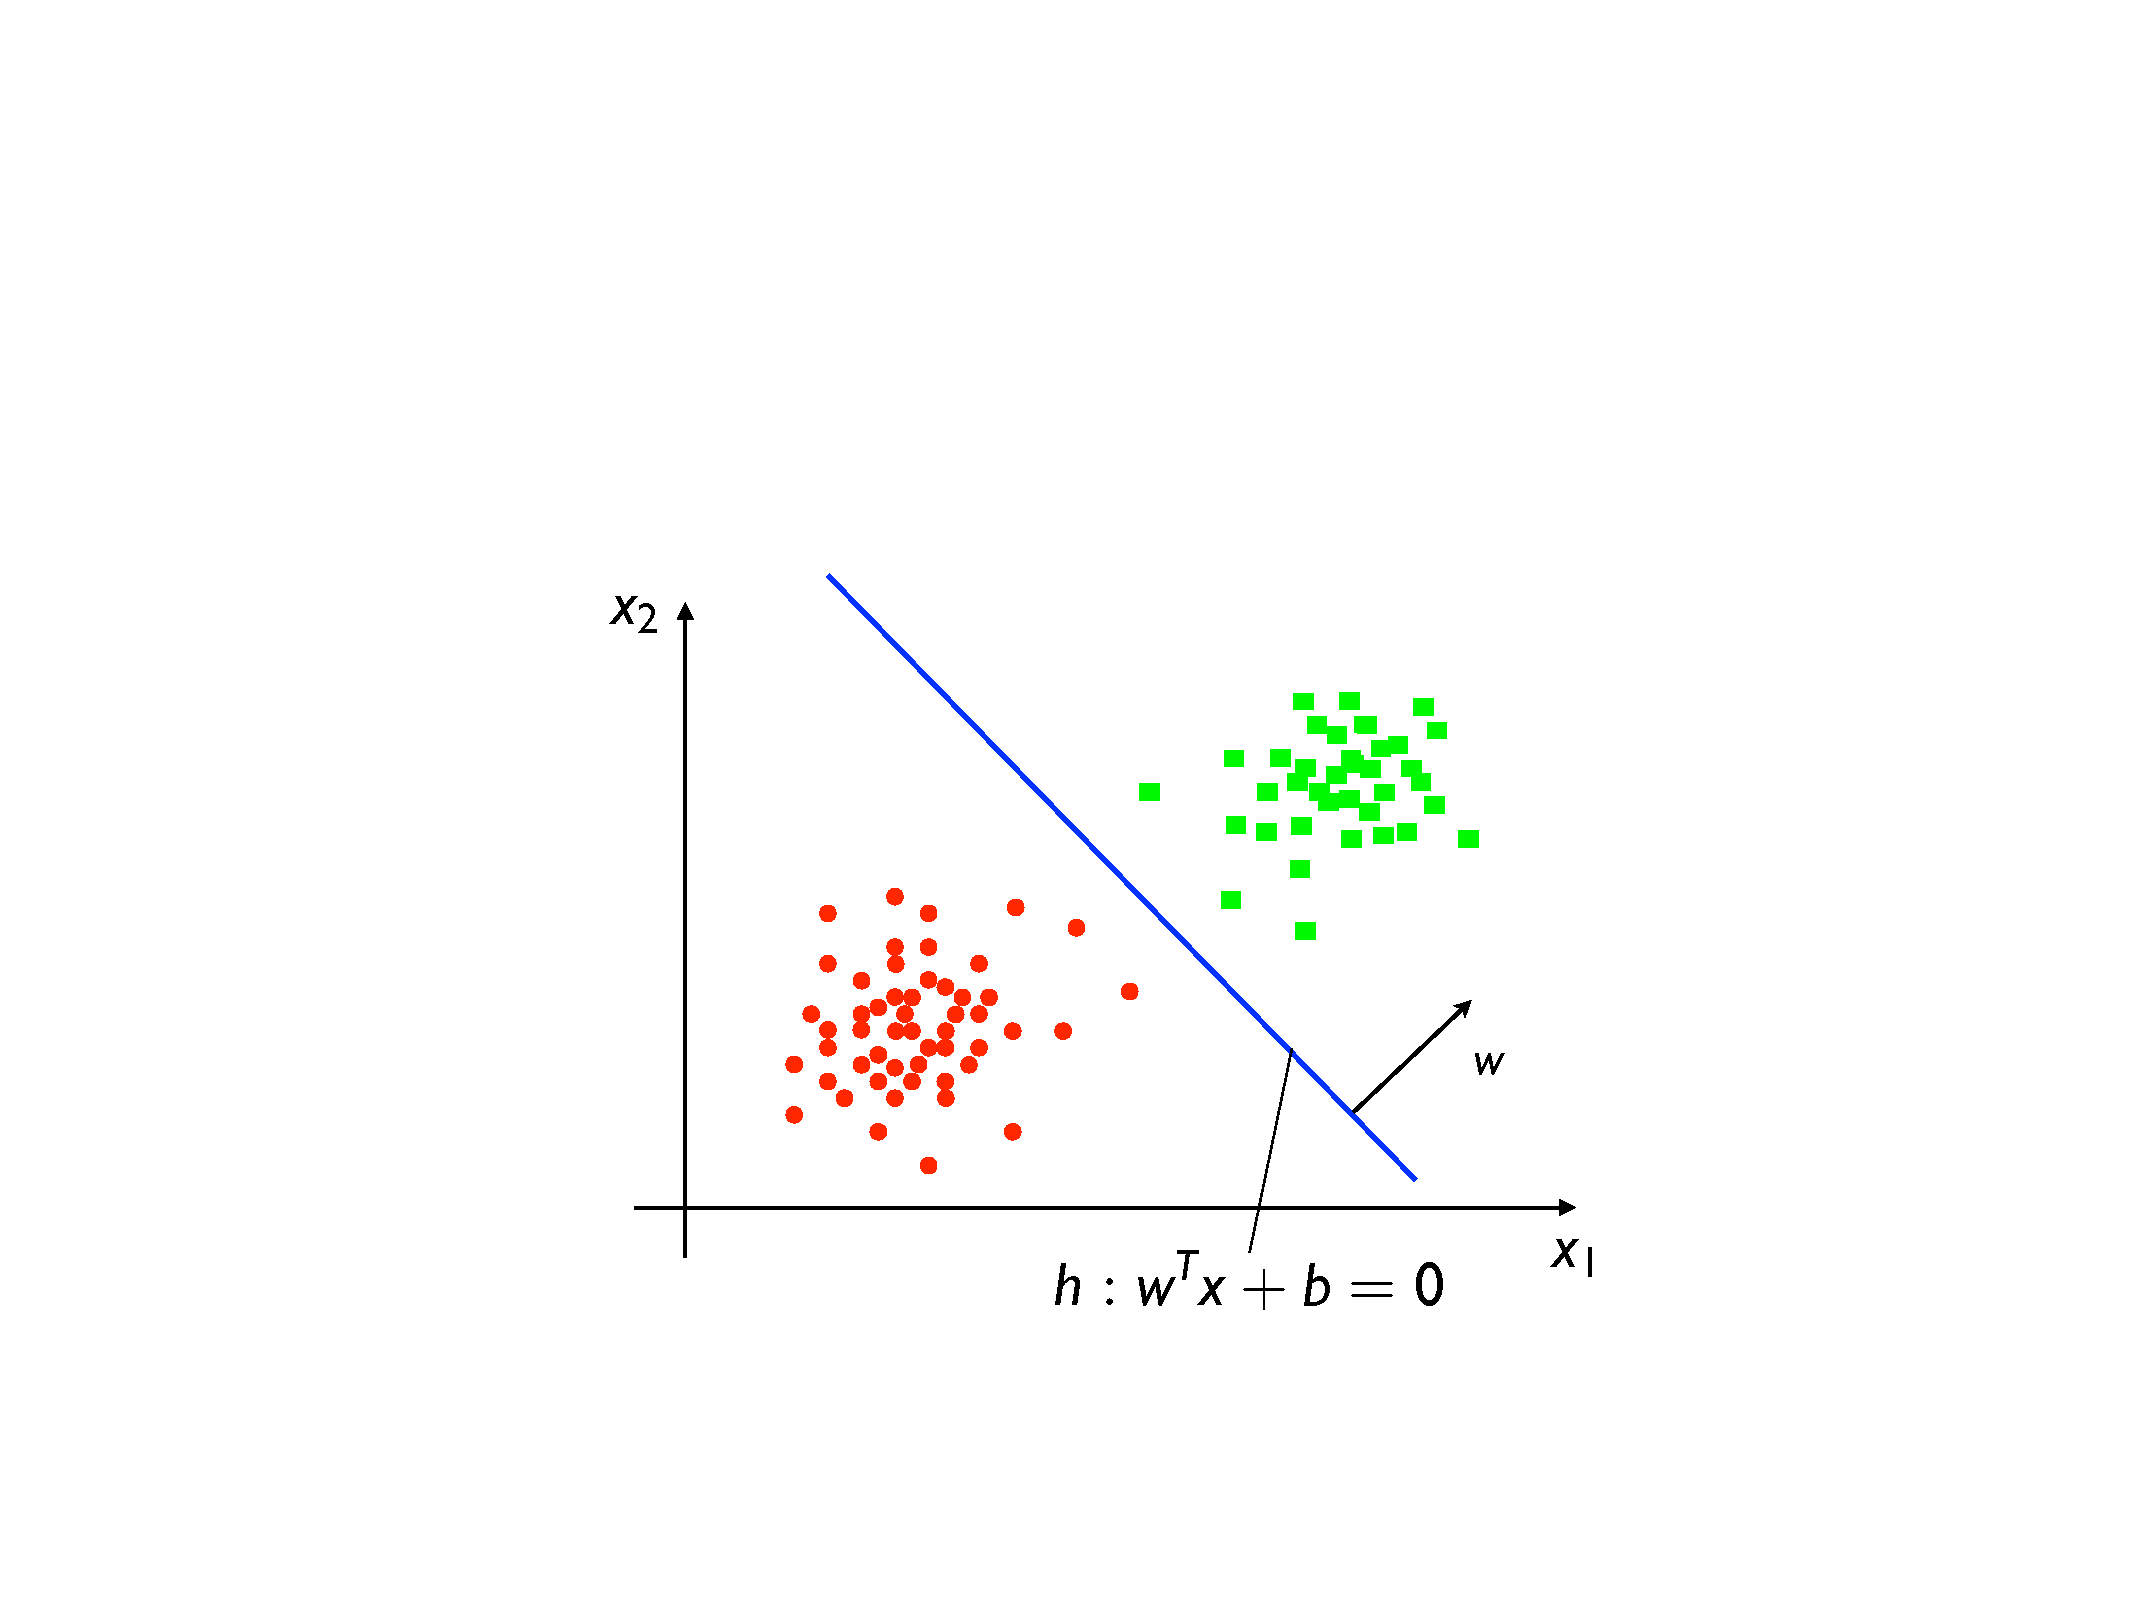
\includegraphics[width=0.7\textwidth]{../graphics/SVM_1a.pdf}
% 	\end{figure}
% 	\begin{itemize}
% 		\item $w^Tx + b  > 0$: $x$ is on the same side as the normal vector $w$ points to.
% 		\item $w^Tx + b  < 0$: $x$ is on the opposite side.
% 		\item With the encoding $y\in\{-1,+1\}$, a sample is correctly classified if $y_i(w^Tx_i + b) > 0$.
% 	\end{itemize}
% \end{frame}

\begin{frame}{Support Vector Machines: linearly separable training set}
	\begin{figure}[htb]
		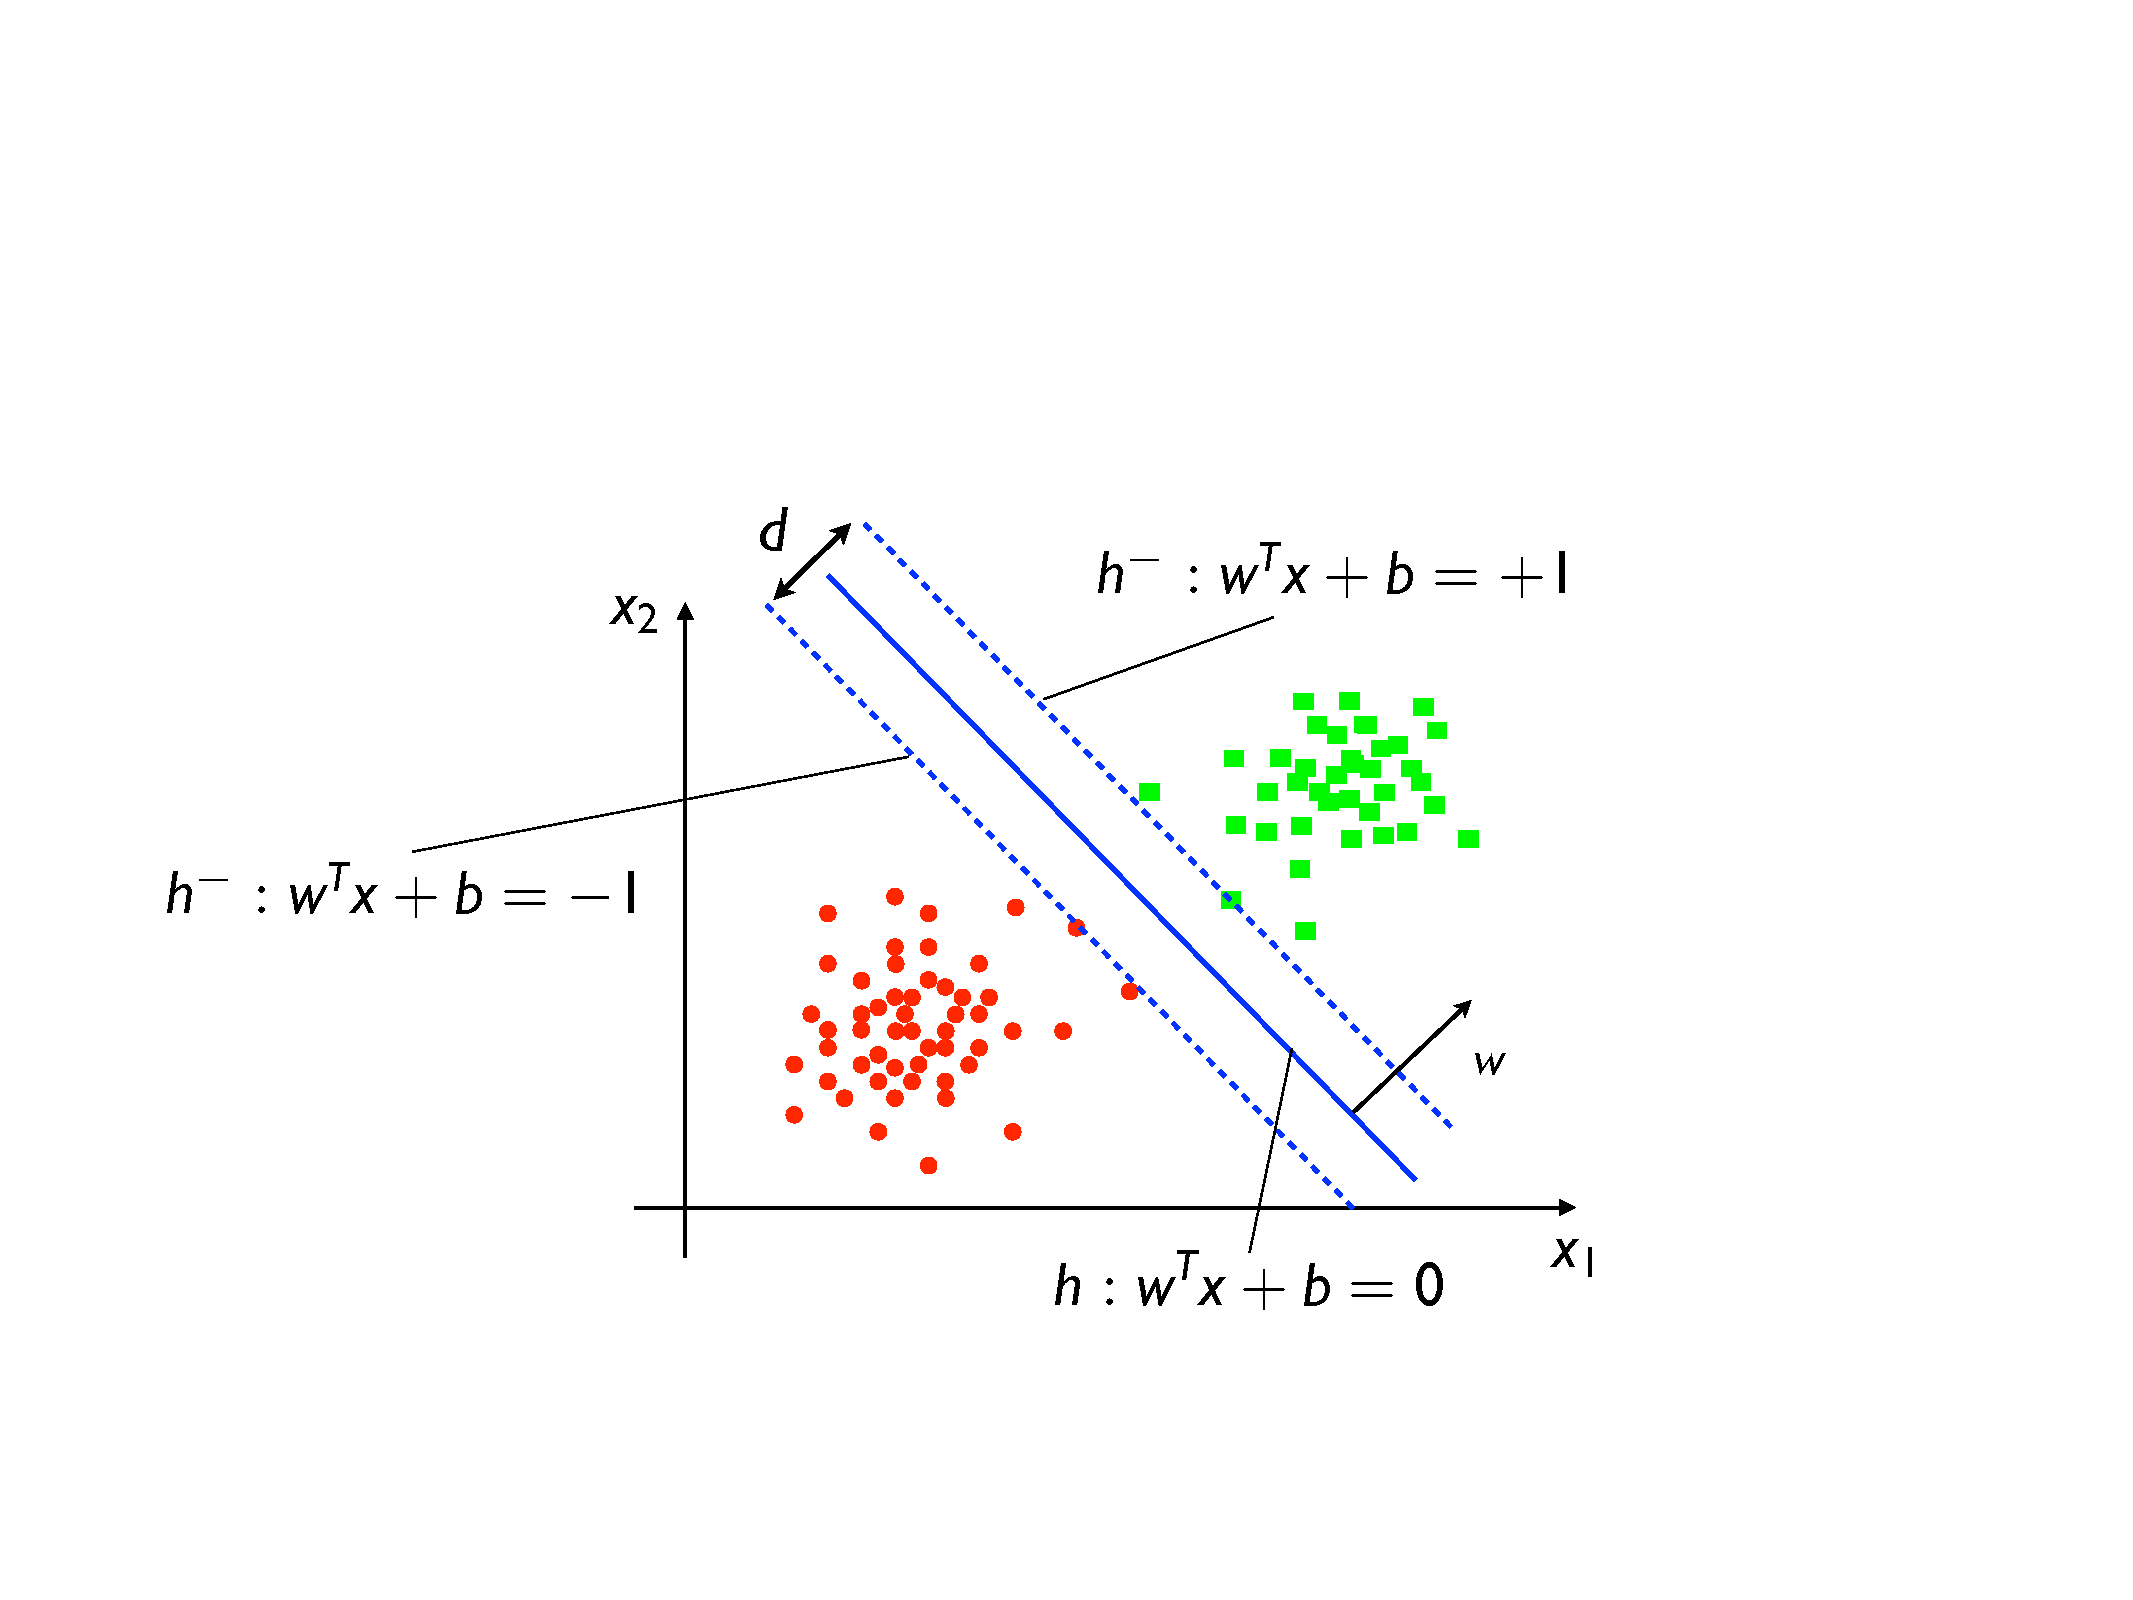
\includegraphics[width=0.7\textwidth]{../graphics/SVM2.pdf}
	\end{figure}
	\begin{itemize}
		\item The ribbon is defined by two parallel lines, for which $w^Tx + b = 1$
		\item The distance between the two parallel lines $w^Tx + b = \pm 1$ is given by
		\begin{equation}
			d = \frac{2}{\|w\|}
		\end{equation}
		\item Maximizing of $d$ is equivalent to minimizing $\|w\|^2$.
	\end{itemize}
\end{frame}


\begin{frame}{Support Vector Machines: linearly separable training set}
	\begin{figure}[htb]
		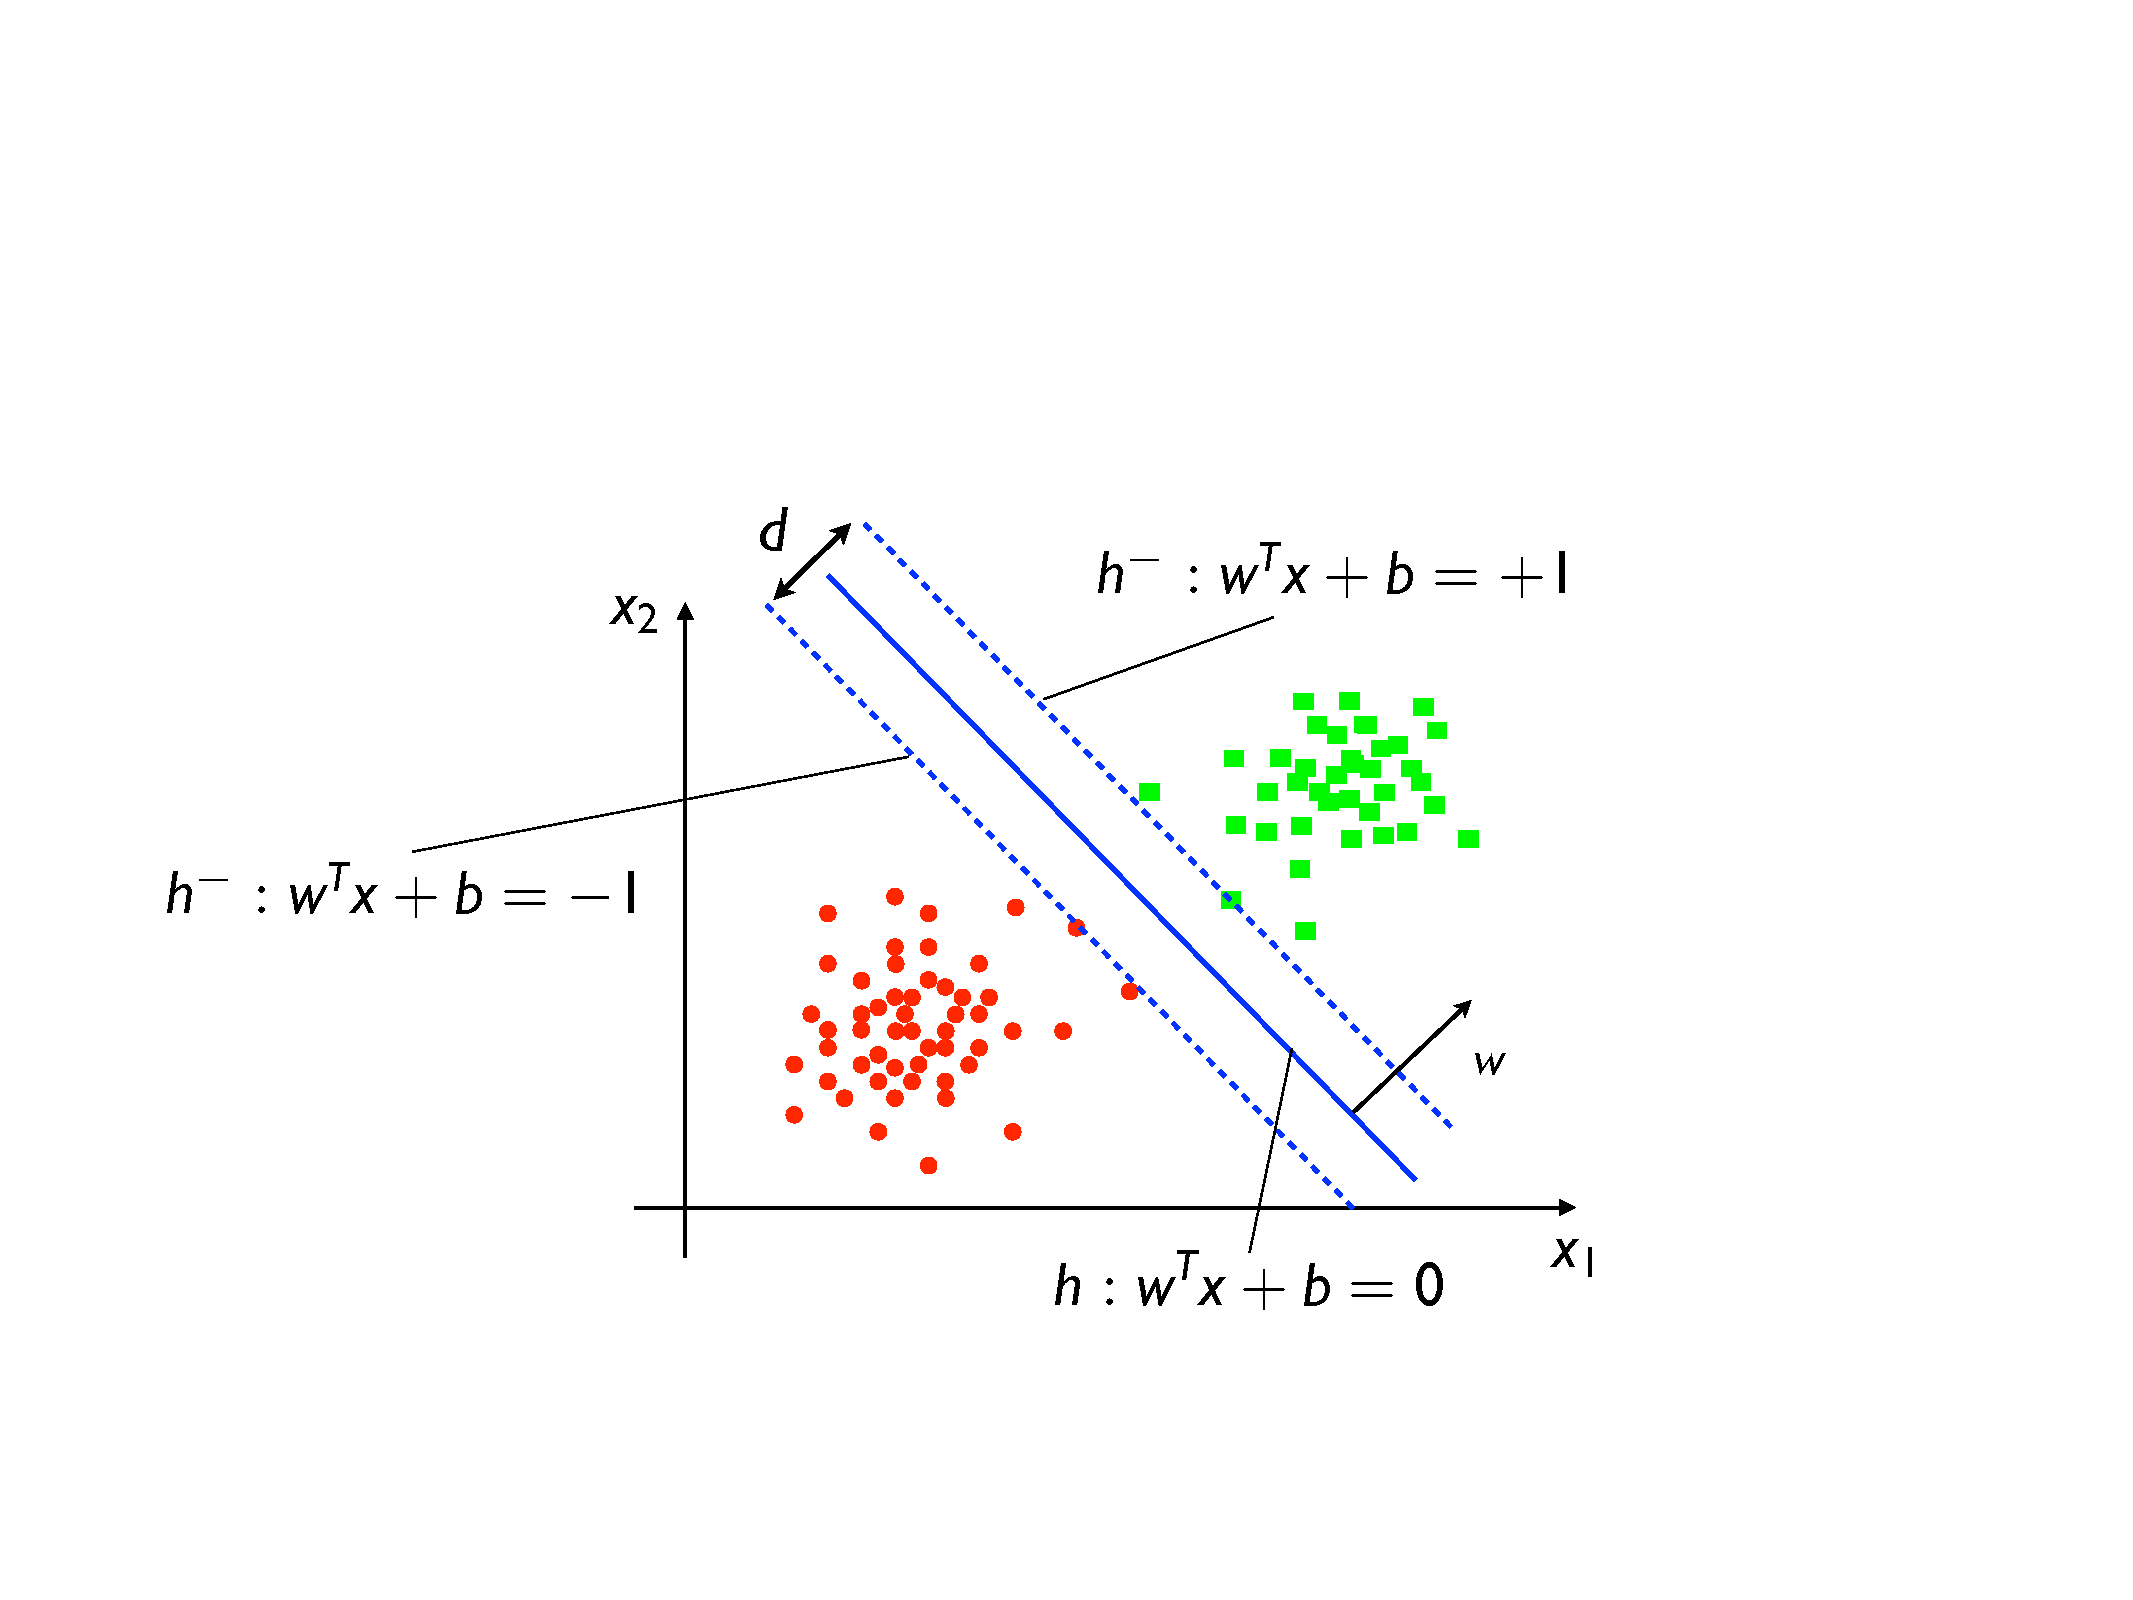
\includegraphics[width=0.7\textwidth]{../graphics/SVM2.pdf}
	\end{figure}
	\begin{itemize}
		\item With this, the problem can be written as a \textbf{convex optimization problem under constraints}:
		\begin{eqnarray*}
			\mbox{minimize} & & \|w\|^2 \\
			\mbox{subject to} & & y_i(w^Tx_i + b) \geq 1 \quad i = 1, \ldots, N
		\end{eqnarray*}
		\item Convexity implies that there is no local minimum besides the global minimum.
	\end{itemize}
\end{frame}


\begin{frame}{SVM for not linearly separable data}
	\begin{figure}[htb]
		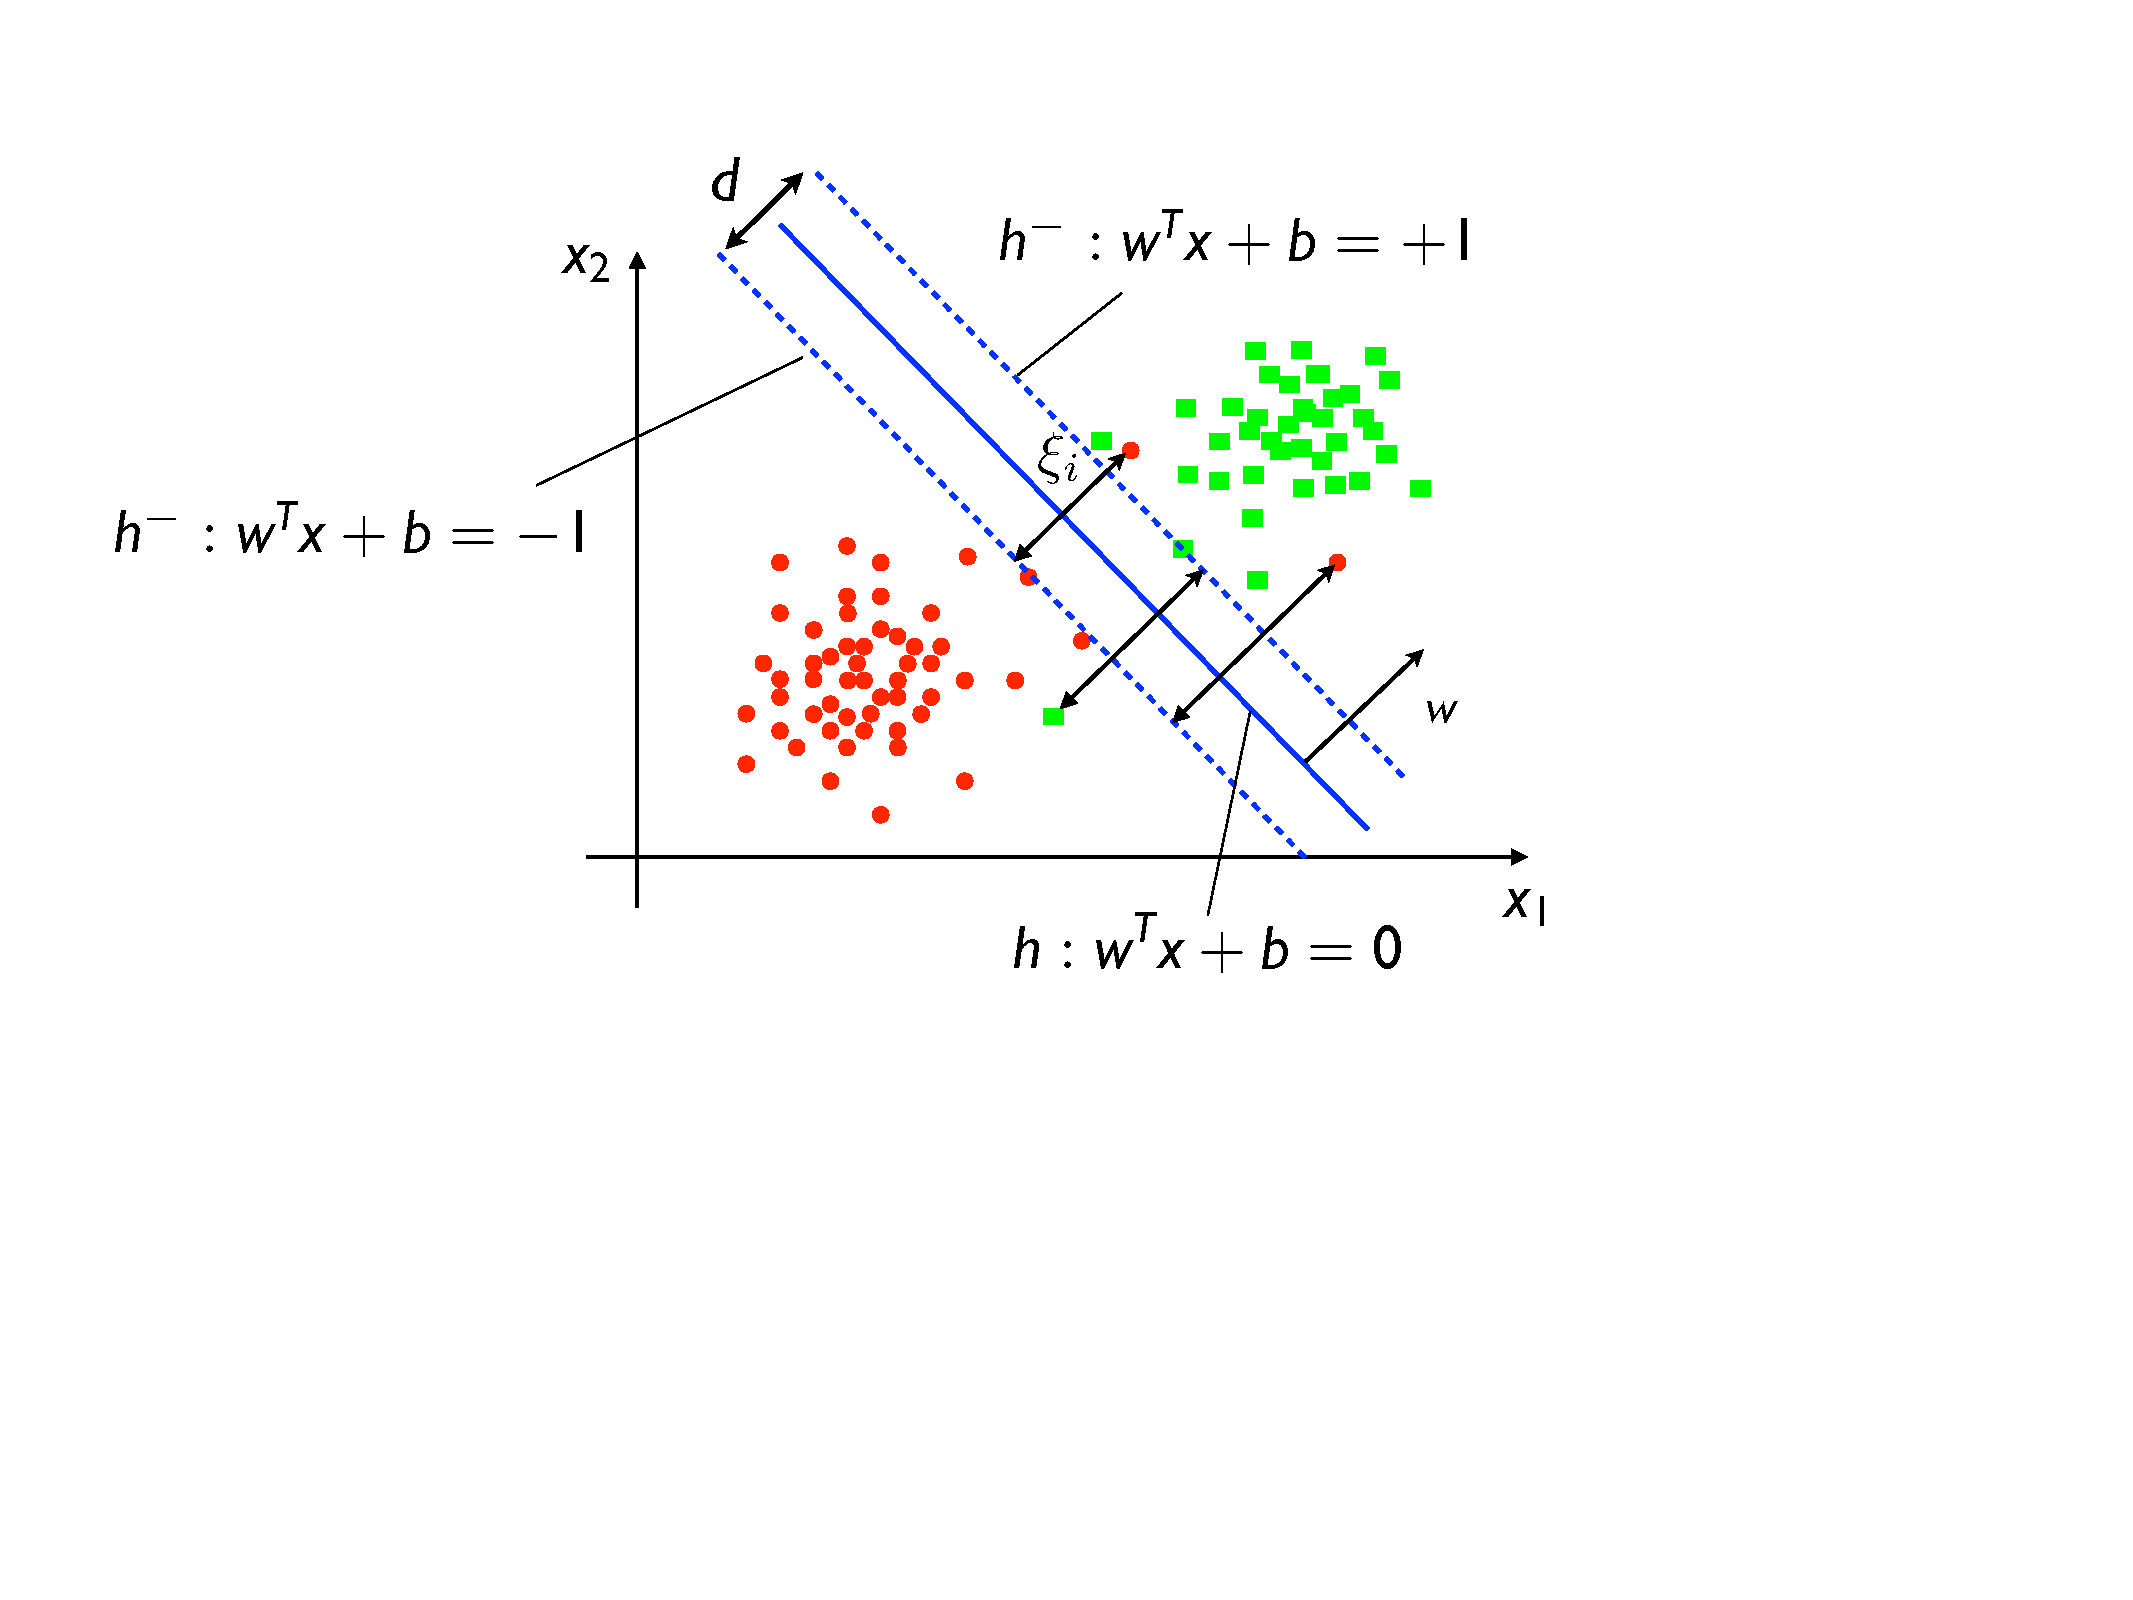
\includegraphics[width=0.7\textwidth]{../graphics/SVM3.pdf}
	\end{figure}
	\begin{itemize}
		\item In reality, complex data is rarely linearly separable.
		\item In this case, we need to find a compromise between error term $\sum_{i=1}^{N}\xi_i$ and regularization $\|w\|^2$ (we omit the constraints):
		\begin{equation*}
			\min_{w,\xi} \|w\|^2 + C \sum_{i=1}^{N}\xi_i
		\end{equation*}
		\item We note that this corresponds to the general formulation we have seen before.
 		\begin{equation*}
 			\param ^{\ast} = \argmin_{\param} \loss (\param) + \lambda \mathcal{R}(\param)
 		\end{equation*}
		\item Normal vector $w$: vector of feature weights.
		\begin{equation*}
			f(x) = w^Tx + b = \sum_{k=1}^{P}w^{(k)}x^{(k)} + b
		\end{equation*}
	\end{itemize}
\end{frame}

% \begin{frame}{SVM for not linearly separable data}
% 	\begin{itemize}
% 		\item SVM correspond to the following constrained optimization problem:
% 		\begin{eqnarray*}
% 			\min_{w,\xi} & & \|w\|^2 + C \sum_{i=1}^{N}\xi_i\\
% 			\mbox{subject to} & & y_i(w^Tx_i + b) \geq 1 - \xi_i \quad i = 1, \ldots, N \\
% 			& & \xi_i \geq 0 \quad i = 1, \ldots, N
% 		\end{eqnarray*}
% 		\item This problem can be efficiently solved with the Lagrange formalism (not shown).
% 		\item We note that this corresponds to the formulation we have seen earlier:
% 		\begin{equation*}
% 			\param ^{\ast} = \argmin_{\param} \loss (\param) + \lambda \mathcal{R}(\param)
% 		\end{equation*}
% 	\end{itemize}
% \end{frame}

\begin{frame}{Support Vector Machines: Kernel trick}
	\begin{figure}[htb]
		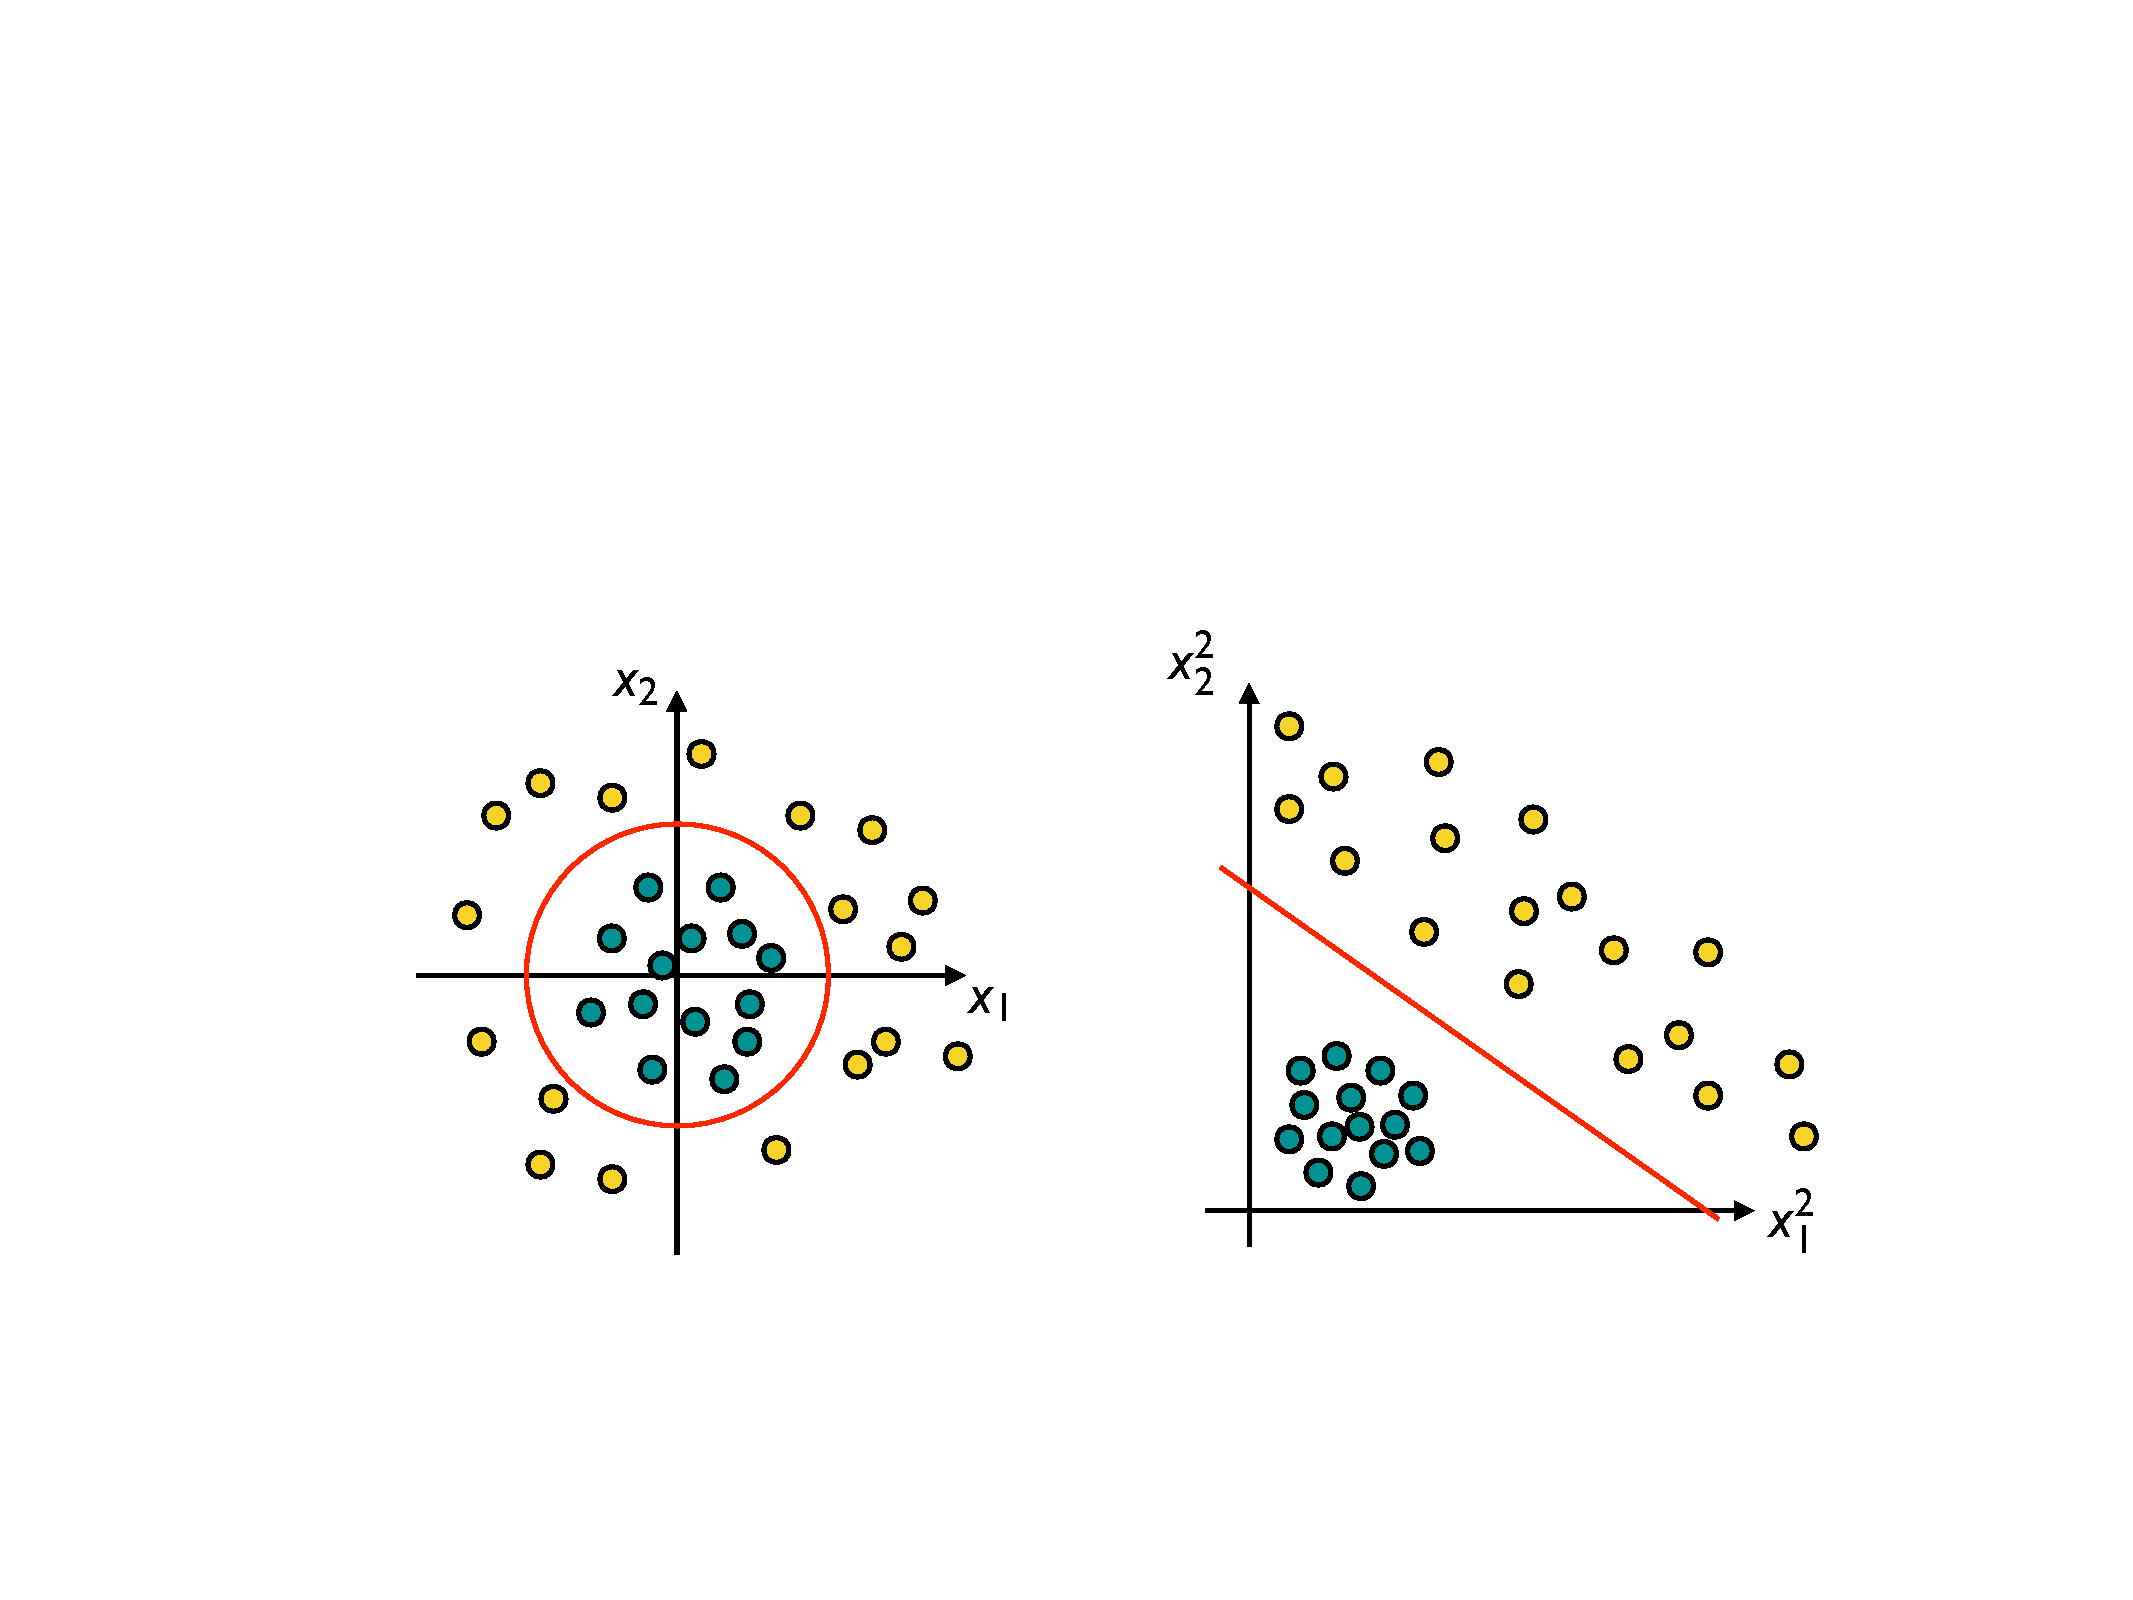
\includegraphics[width=0.7\textwidth]{../graphics/KernelTrick.pdf}
	\end{figure}
	\begin{itemize}
		\item Limitation: linear decision boundaries
		\item Solution: transform the features in a higher dimensional space.
		\item SVM: in-built mechanism to do such transformations efficiently.
		\item Finding good representations is at the very heart of Neural Networks.
	\end{itemize}
\end{frame}

% \begin{frame}{How to set hyperparameters ... }
% 	\begin{itemize}
% 		\item Training a classifier: finding automatically a large number of feature weights (SVM, LDA) or other parameters (RF) from annotated data.
% 		\item Hyperparameters: a small number of parameters that are set to control the training process, such as the number of trees, or the regularization parameter $\lambda$ ($C$ in SVM).
% 		\item The question is: how can we find good hyperparameters?
% 		\item Strategy: grid search. We choose the set of hyperparameters that perform best (i.e. that lead to the classifier with the best performance).
% 		\item Problem: how can we measure the performance?
% 	\end{itemize}
% \end{frame}

\section{Conclusion}
\begin{frame}{Conclusion}
	\begin{itemize}
		\item Supervised Machine Learning is concerned with inferring a function $f$ from a set of annotated data, allowing to predict some output variable $y$ from inputs $x$.
		%% \item Different views:
		%% 	\begin{itemize}
		%% 		\item Probabilistic view: we maximize the posterior probability.
		%% 		\item Discriminant view: we optimize the separation of classes.
		%% 	\end{itemize}
		\item Compromise: we want to minimize the error and regularize $f$.
		\item Forms of regularization we have seen so far:
			\begin{itemize}
				\item Regularization by model averaging (e.g. RF)
				\item Minimizing a global loss function containing an error and a regularization term:
				\begin{equation*}
					\param ^{\ast} = \argmin_{\param} \loss (\param) + \lambda \mathcal{R}(\param)
				\end{equation*}
			\end{itemize}
		\item All the methods, we have seen so far work on a fixed representation of the objects (often a vector $x \in\mathbb{R}^P$).
	\end{itemize}
\end{frame}

%%%%%%%%%%%%%%%%%%%%%%%%%%%%%%%%%%%%%%%%%%%%%%%%%%%%%%%%%%%%%%%%%%%%%%%%%
%%%%%%%%%%%%%%%%%%%%%%%%%%%%%%%%%%%%%%%%%%%%%%%%%%%%%%%%%%%%%%%%%%%%%%%%%
\section{References}
\begin{frame}[allowframebreaks]
	\frametitle{References}
	\bibliography{slides_deep.bib}
\end{frame}


\end{document}
